% Options for packages loaded elsewhere
% Options for packages loaded elsewhere
\PassOptionsToPackage{unicode}{hyperref}
\PassOptionsToPackage{hyphens}{url}
\PassOptionsToPackage{dvipsnames,svgnames,x11names}{xcolor}
%
\documentclass[
  letterpaper,
  DIV=11,
  numbers=noendperiod]{scrartcl}
\usepackage{xcolor}
\usepackage{amsmath,amssymb}
\setcounter{secnumdepth}{5}
\usepackage{iftex}
\ifPDFTeX
  \usepackage[T1]{fontenc}
  \usepackage[utf8]{inputenc}
  \usepackage{textcomp} % provide euro and other symbols
\else % if luatex or xetex
  \usepackage{unicode-math} % this also loads fontspec
  \defaultfontfeatures{Scale=MatchLowercase}
  \defaultfontfeatures[\rmfamily]{Ligatures=TeX,Scale=1}
\fi
\usepackage{lmodern}
\ifPDFTeX\else
  % xetex/luatex font selection
\fi
% Use upquote if available, for straight quotes in verbatim environments
\IfFileExists{upquote.sty}{\usepackage{upquote}}{}
\IfFileExists{microtype.sty}{% use microtype if available
  \usepackage[]{microtype}
  \UseMicrotypeSet[protrusion]{basicmath} % disable protrusion for tt fonts
}{}
\makeatletter
\@ifundefined{KOMAClassName}{% if non-KOMA class
  \IfFileExists{parskip.sty}{%
    \usepackage{parskip}
  }{% else
    \setlength{\parindent}{0pt}
    \setlength{\parskip}{6pt plus 2pt minus 1pt}}
}{% if KOMA class
  \KOMAoptions{parskip=half}}
\makeatother
% Make \paragraph and \subparagraph free-standing
\makeatletter
\ifx\paragraph\undefined\else
  \let\oldparagraph\paragraph
  \renewcommand{\paragraph}{
    \@ifstar
      \xxxParagraphStar
      \xxxParagraphNoStar
  }
  \newcommand{\xxxParagraphStar}[1]{\oldparagraph*{#1}\mbox{}}
  \newcommand{\xxxParagraphNoStar}[1]{\oldparagraph{#1}\mbox{}}
\fi
\ifx\subparagraph\undefined\else
  \let\oldsubparagraph\subparagraph
  \renewcommand{\subparagraph}{
    \@ifstar
      \xxxSubParagraphStar
      \xxxSubParagraphNoStar
  }
  \newcommand{\xxxSubParagraphStar}[1]{\oldsubparagraph*{#1}\mbox{}}
  \newcommand{\xxxSubParagraphNoStar}[1]{\oldsubparagraph{#1}\mbox{}}
\fi
\makeatother


\usepackage{longtable,booktabs,array}
\usepackage{calc} % for calculating minipage widths
% Correct order of tables after \paragraph or \subparagraph
\usepackage{etoolbox}
\makeatletter
\patchcmd\longtable{\par}{\if@noskipsec\mbox{}\fi\par}{}{}
\makeatother
% Allow footnotes in longtable head/foot
\IfFileExists{footnotehyper.sty}{\usepackage{footnotehyper}}{\usepackage{footnote}}
\makesavenoteenv{longtable}
\usepackage{graphicx}
\makeatletter
\newsavebox\pandoc@box
\newcommand*\pandocbounded[1]{% scales image to fit in text height/width
  \sbox\pandoc@box{#1}%
  \Gscale@div\@tempa{\textheight}{\dimexpr\ht\pandoc@box+\dp\pandoc@box\relax}%
  \Gscale@div\@tempb{\linewidth}{\wd\pandoc@box}%
  \ifdim\@tempb\p@<\@tempa\p@\let\@tempa\@tempb\fi% select the smaller of both
  \ifdim\@tempa\p@<\p@\scalebox{\@tempa}{\usebox\pandoc@box}%
  \else\usebox{\pandoc@box}%
  \fi%
}
% Set default figure placement to htbp
\def\fps@figure{htbp}
\makeatother





\setlength{\emergencystretch}{3em} % prevent overfull lines

\providecommand{\tightlist}{%
  \setlength{\itemsep}{0pt}\setlength{\parskip}{0pt}}



 


\KOMAoption{captions}{tableheading}
\makeatletter
\@ifpackageloaded{caption}{}{\usepackage{caption}}
\AtBeginDocument{%
\ifdefined\contentsname
  \renewcommand*\contentsname{Table of contents}
\else
  \newcommand\contentsname{Table of contents}
\fi
\ifdefined\listfigurename
  \renewcommand*\listfigurename{List of Figures}
\else
  \newcommand\listfigurename{List of Figures}
\fi
\ifdefined\listtablename
  \renewcommand*\listtablename{List of Tables}
\else
  \newcommand\listtablename{List of Tables}
\fi
\ifdefined\figurename
  \renewcommand*\figurename{Figure}
\else
  \newcommand\figurename{Figure}
\fi
\ifdefined\tablename
  \renewcommand*\tablename{Table}
\else
  \newcommand\tablename{Table}
\fi
}
\@ifpackageloaded{float}{}{\usepackage{float}}
\floatstyle{ruled}
\@ifundefined{c@chapter}{\newfloat{codelisting}{h}{lop}}{\newfloat{codelisting}{h}{lop}[chapter]}
\floatname{codelisting}{Listing}
\newcommand*\listoflistings{\listof{codelisting}{List of Listings}}
\makeatother
\makeatletter
\makeatother
\makeatletter
\@ifpackageloaded{caption}{}{\usepackage{caption}}
\@ifpackageloaded{subcaption}{}{\usepackage{subcaption}}
\makeatother
\usepackage{bookmark}
\IfFileExists{xurl.sty}{\usepackage{xurl}}{} % add URL line breaks if available
\urlstyle{same}
\hypersetup{
  pdftitle={Quantifying comprehensive marine vessel emissions using data fusion},
  pdfauthor={emLab, UCSB and GFW},
  colorlinks=true,
  linkcolor={blue},
  filecolor={Maroon},
  citecolor={Blue},
  urlcolor={Blue},
  pdfcreator={LaTeX via pandoc}}


\title{Quantifying comprehensive marine vessel emissions using data
fusion}
\author{emLab, UCSB and GFW}
\date{Last Updated on January 22, 2026}
\begin{document}
\maketitle

\renewcommand*\contentsname{Table of contents}
{
\hypersetup{linkcolor=}
\setcounter{tocdepth}{3}
\tableofcontents
}

\begin{verbatim}
Reading layer `World_Countries_Generalized' from data source 
  `/Users/gmcdonald/github/paper-ocean-ghg/data/World_Countries_Generalized_Shapefile/World_Countries_Generalized.shp' 
  using driver `ESRI Shapefile'
Simple feature collection with 251 features and 4 fields
Geometry type: MULTIPOLYGON
Dimension:     XY
Bounding box:  xmin: -20037510 ymin: -30240970 xmax: 20037510 ymax: 18418390
Projected CRS: WGS 84 / Pseudo-Mercator
\end{verbatim}

\begin{figure}[H]

\centering{

\pandocbounded{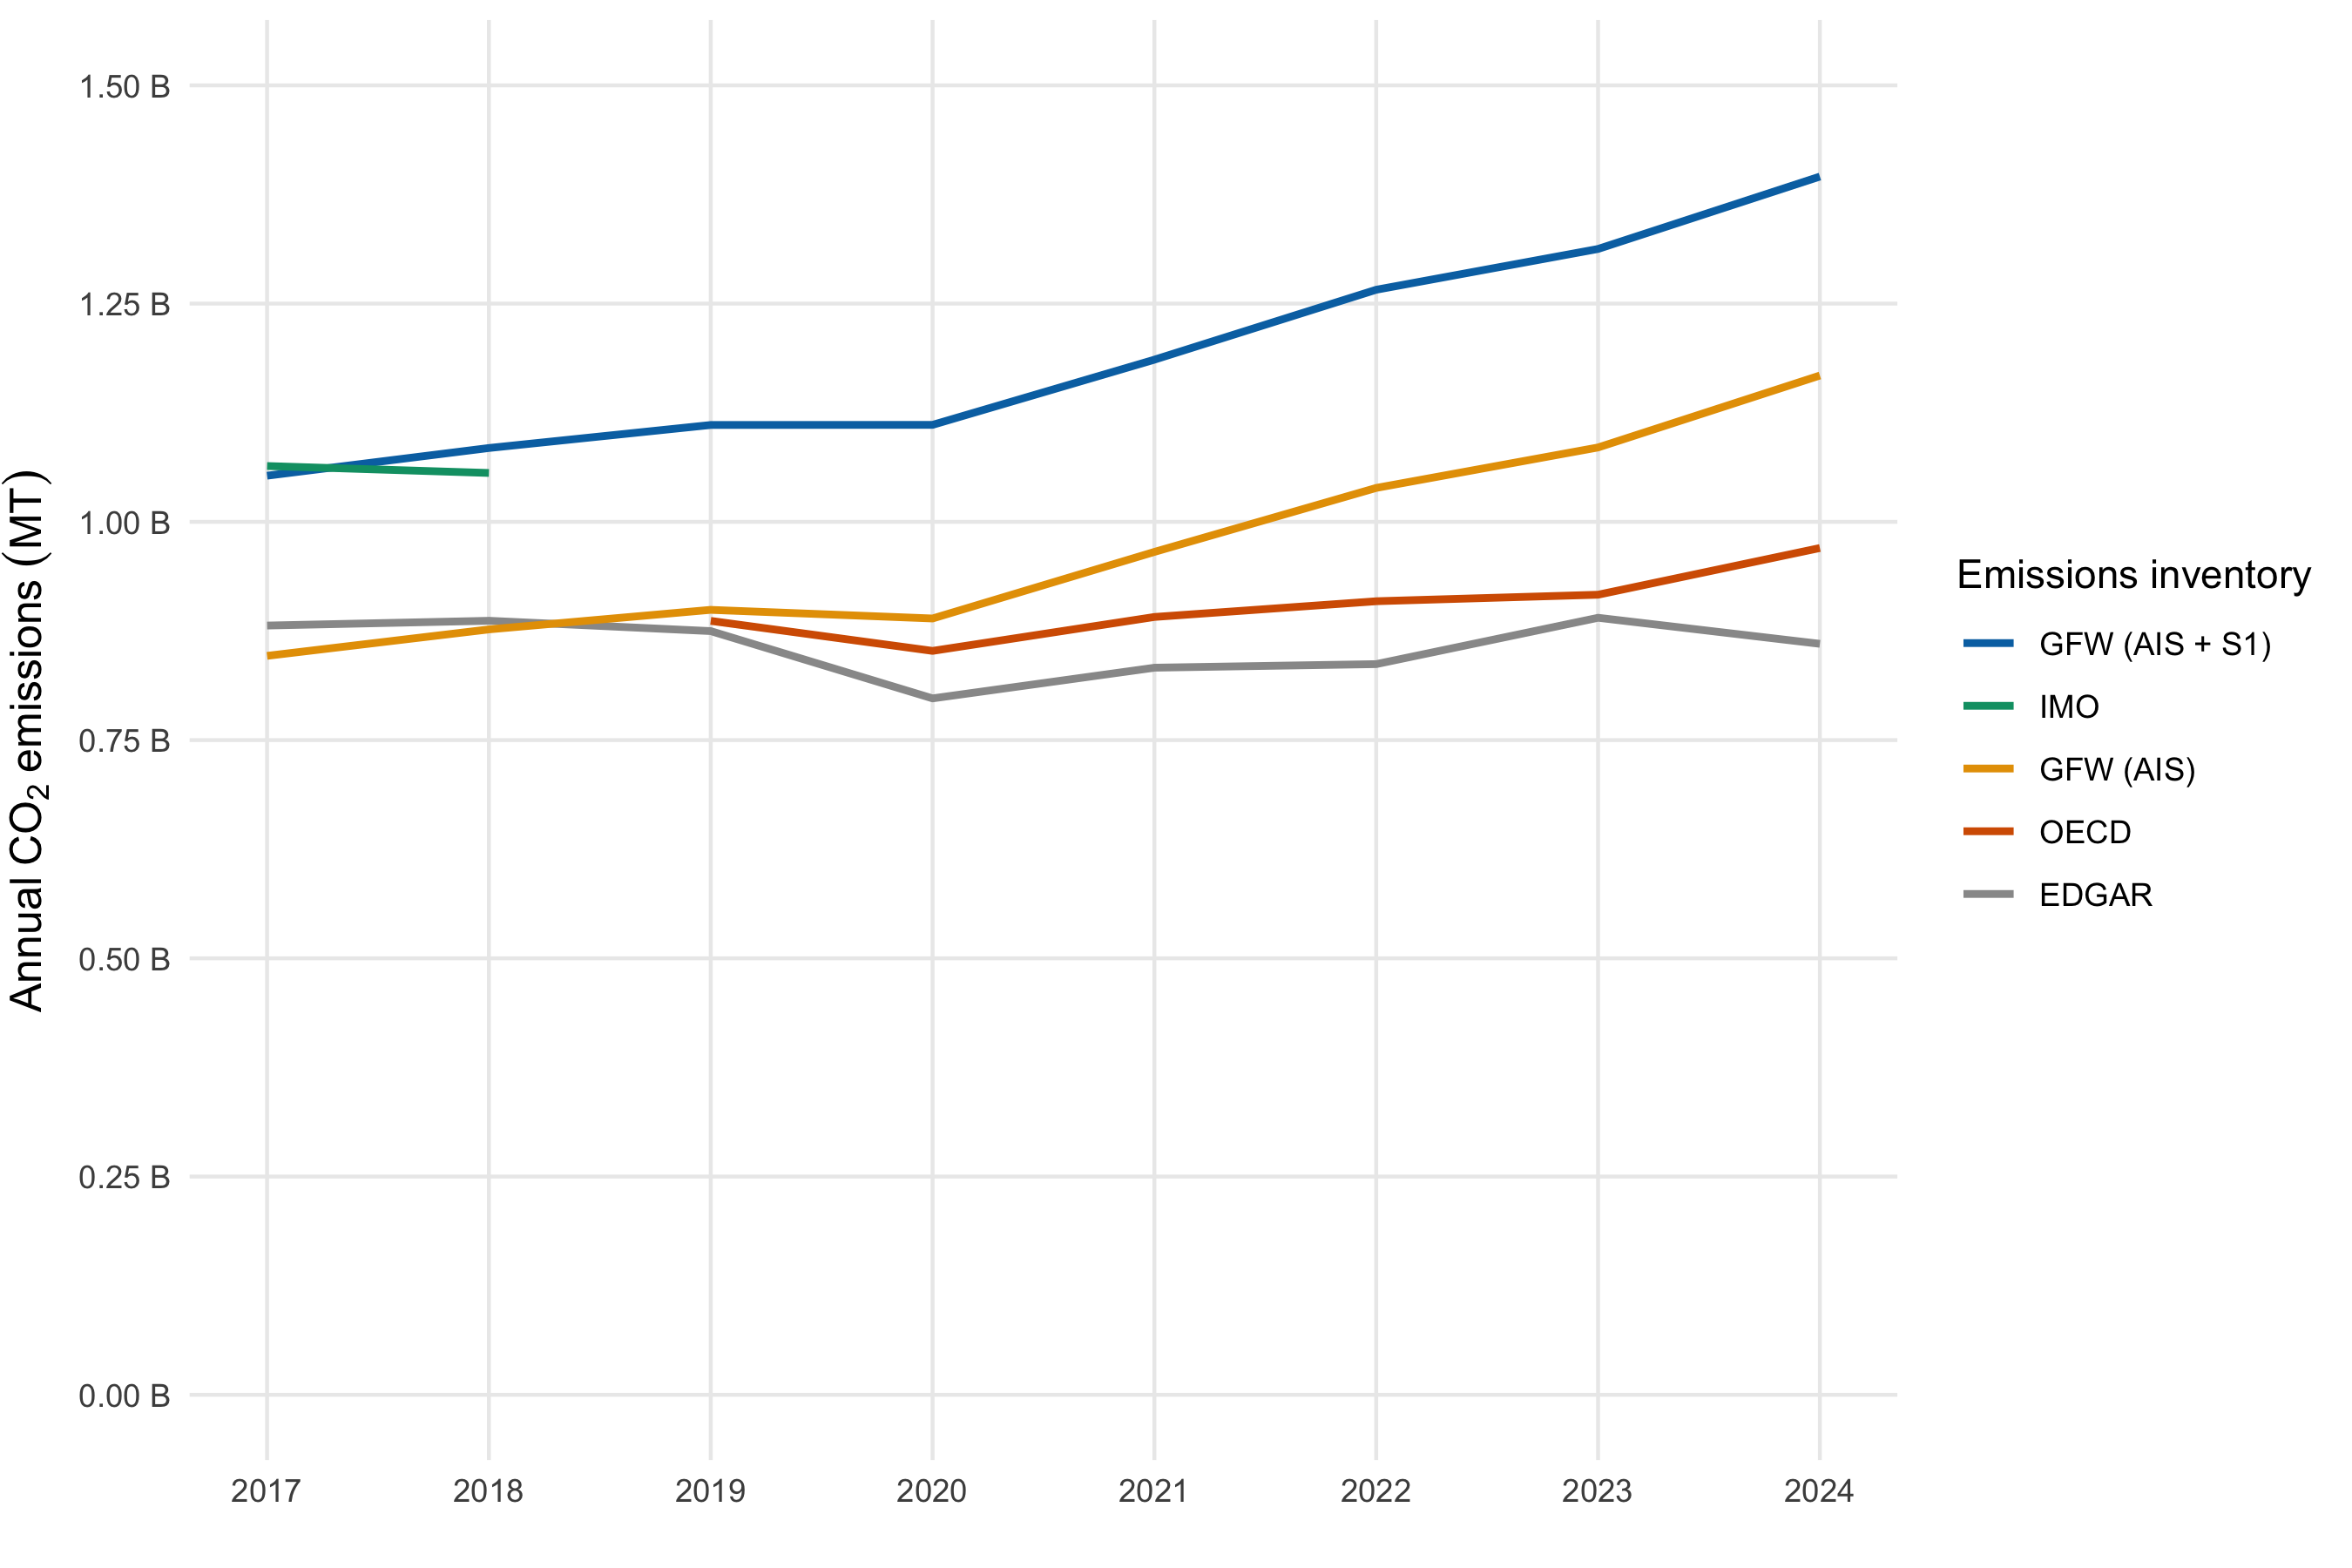
\includegraphics[keepaspectratio]{../figures/fig-inventory-comparison-1.png}}

}

\caption{\label{fig-inventory-comparison}}

\end{figure}%

\# In-line manuscript statistics

\begin{itemize}
\item
  The transportation sector is a major source of global greenhouse gas
  (GHG) and local air pollution emissions, responsible for 21\% of all
  CO\(_{2}\) emissions globally in 2024
\item
  For over 880,000 AIS-broadcasting vessels, we quantify point-estimate
  emissions for each vessel using precise latitude/longitude/timestamp
  information for over 94 billion individual AIS messages

  \begin{itemize}
  \tightlist
  \item
    We obtained a dataset containing 29.2 million vessel detections from
    2017 to 2024, of which 13.5 million detections were not matched to a
    broadcasting vessel. These detections come from across more than 845
    individual S1 scenes.
  \end{itemize}
\item
  Because many vessels do not broadcast AIS, current approaches solely
  based on AIS \textit{underestimate} current global emissions by 8.36\%
  (in 2024), and \textit{overestimate} the increasing trend by 17.78\%
  (from 2017 to 2024).
\item
  Using the latest data available from the EU's Emissions Database for
  Global Atmospheric Research (EDGAR), we estimate that in 2024 marine
  vessels accounted for 15\% of all transportation-related CO\(_{2}\)
  emissions. Marine vessel CO\(_{2}\) emissions increased by 32.2\%
  between 2017 and 2024, 10 times faster than the growth rate of other
  transportation emissions, and 5 faster than the growth rate of total
  global emissions across all sectors.
\item
  Across the entire 2017 to 2024 time series, 94.6\% of non-broadcasting
  emissions occurred inside the S1 footprint and in pixel-months that
  were imaged; 5.4\% occurred inside the S1 footprint but in
  pixel-months that weren't imaged; and 0.006\% occurred outside the S1
  footprint entirely.
\item
  In 2024, 23.0\% of CO\(_{2}\) emissions from fishing vessels were from
  non-broadcasting vessels, and 7.2\% of CO\(_{2}\) emissions from
  non-fishing vessels were from non-broadcasting vessels. For both types
  of vessels, this fraction of emissions from non-broadcasting vessels
  has been declining steadily since 2020.

  \begin{itemize}
  \tightlist
  \item
    The total social cost of CO\(_{2}\), CH\(_{4}\), and N\(_{2}\)O
    emissions in 2024 was 311 billion USD. This represents about 5\% of
    the total value of all goods transported by maritime trade (using
    6.63 trillion USD as the 2021 value of maritime-traded goods).
  \end{itemize}

  \section{Figures}\label{figures}

  \subsection{Figure 1}\label{figure-1}

  \subsubsection{Figure 1, panel A}\label{figure-1-panel-a}
\end{itemize}

\subsubsection{Figure 2, panel B}\label{figure-2-panel-b}

\subsubsection{Figure 1, panel A}\label{figure-1-panel-a-1}

\subsubsection{Figure 1, combined}\label{figure-1-combined}

\begin{figure}[H]

\centering{

\pandocbounded{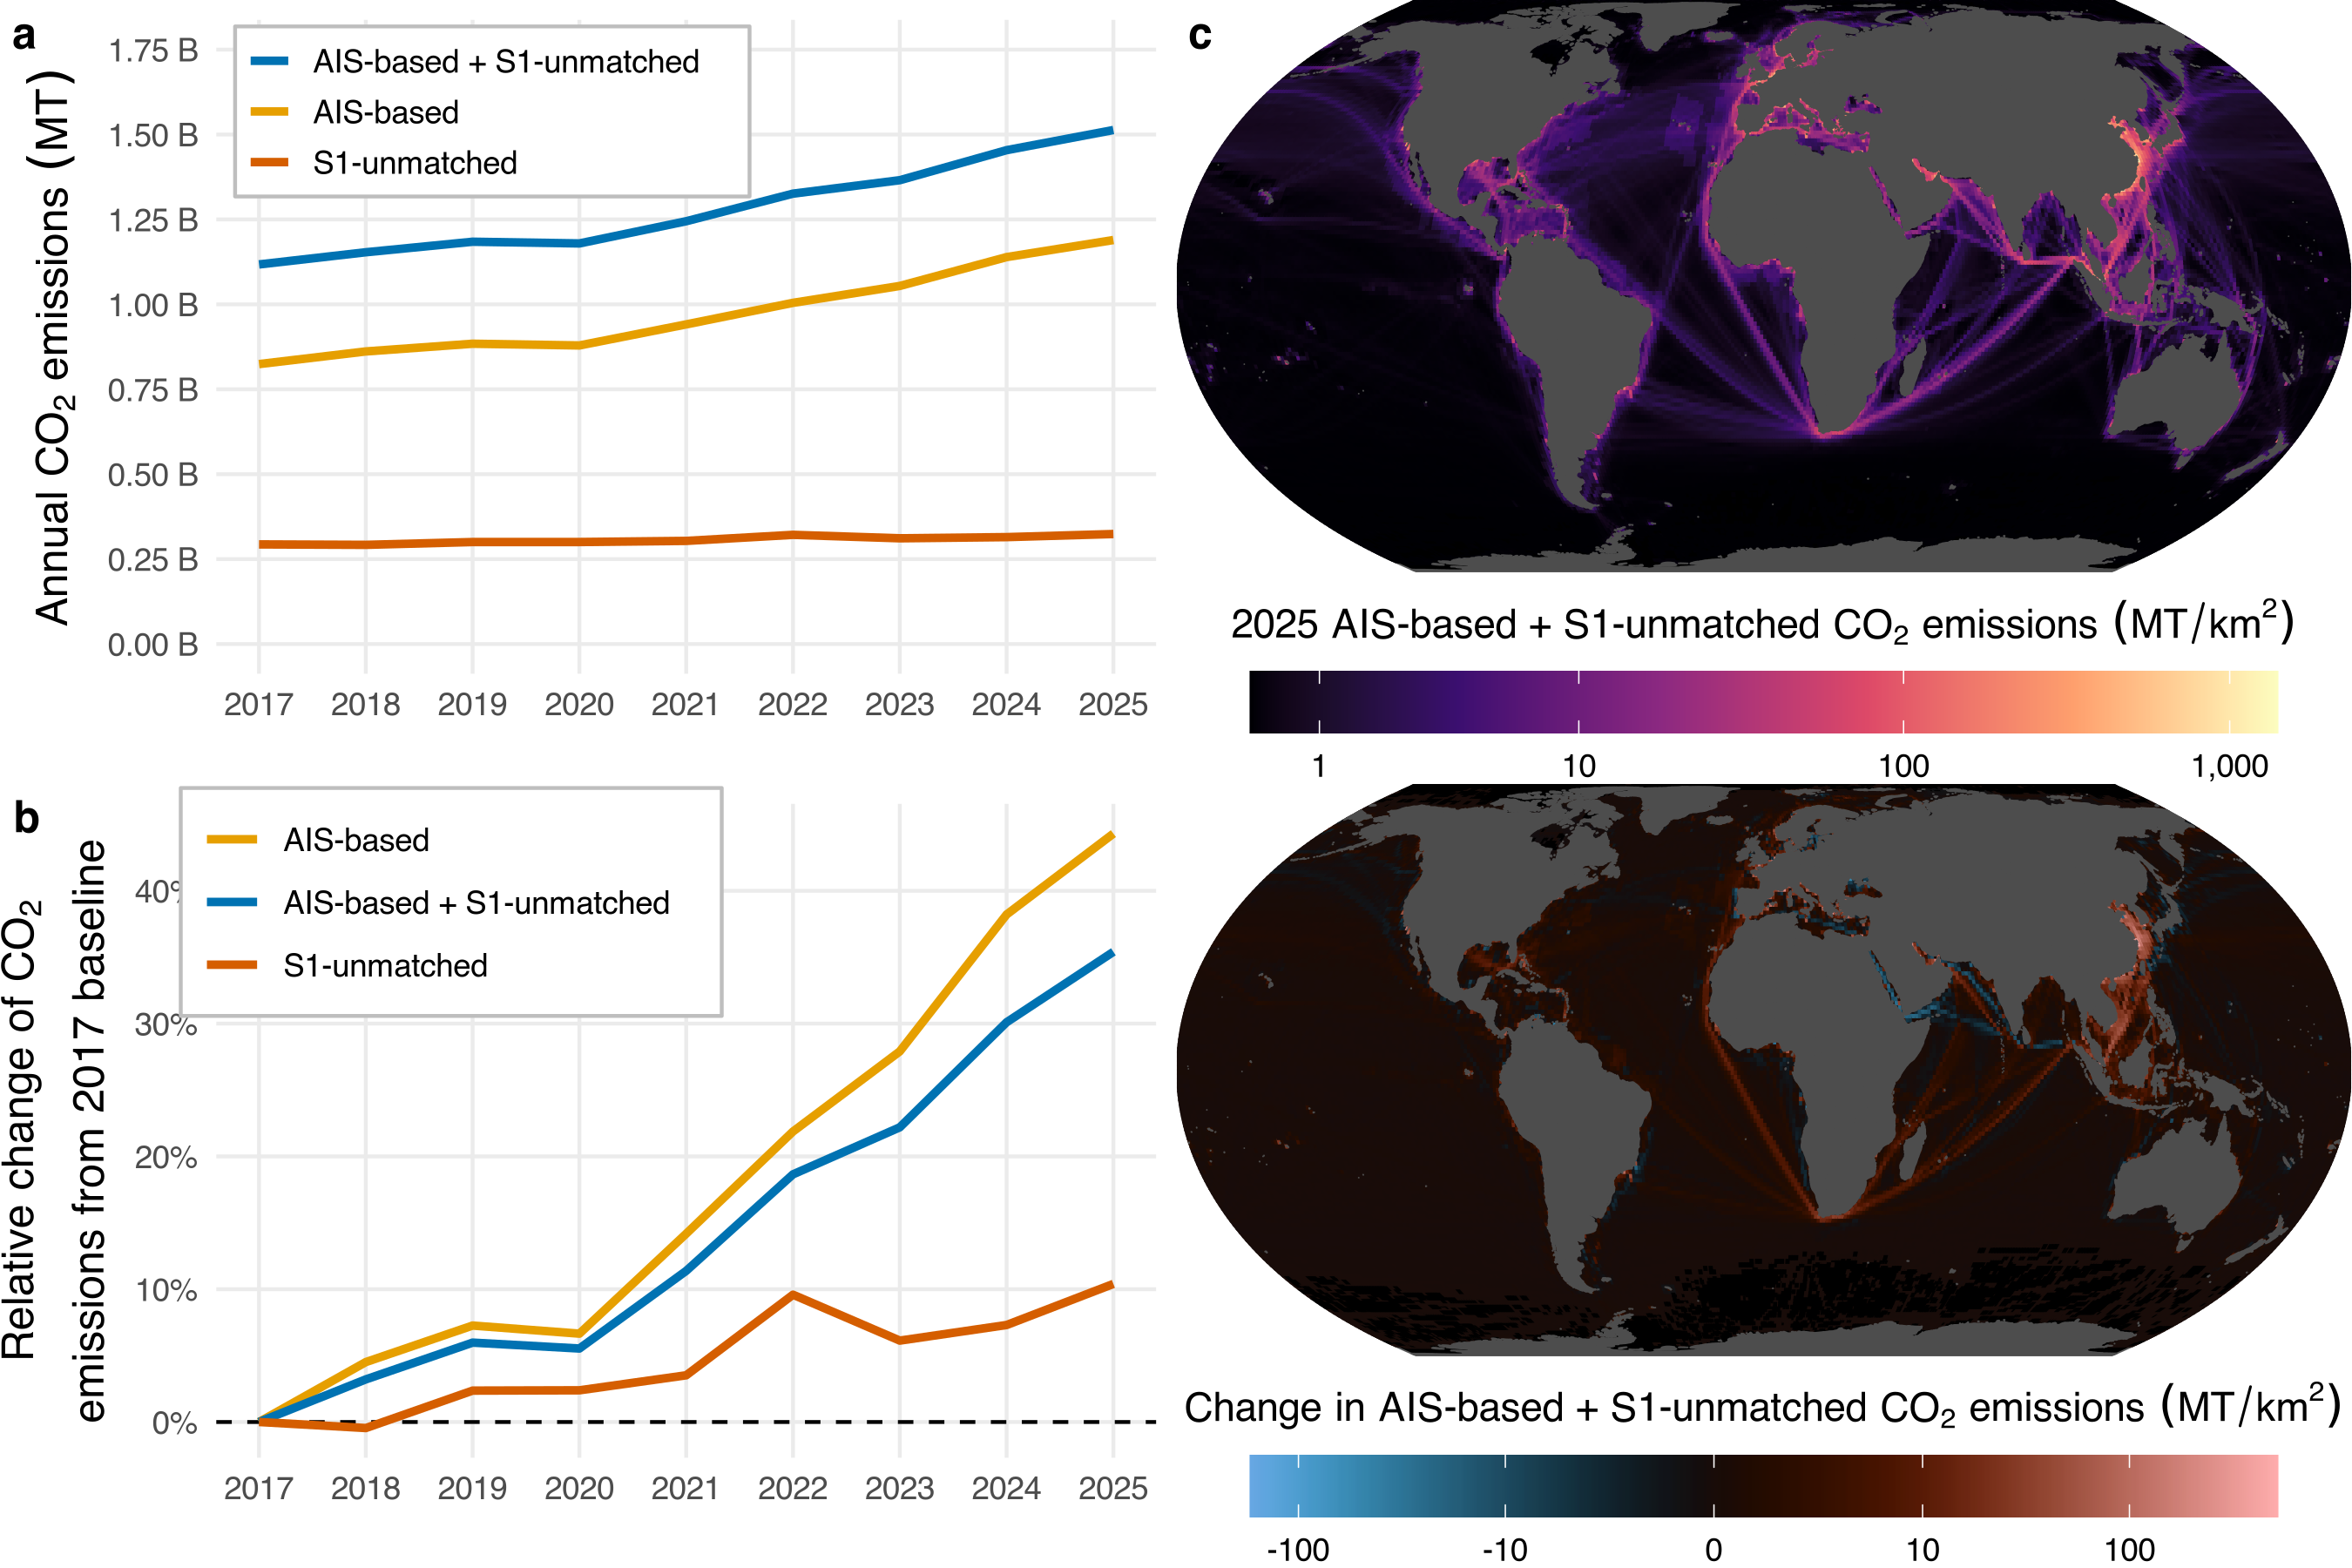
\includegraphics[keepaspectratio]{../figures/fig-emissions-by-data-source-and-maps-1.png}}

}

\caption{\label{fig-emissions-by-data-source-and-maps}}

\end{figure}%

\subsubsection{Figure 2}\label{figure-2}

\begin{figure}[H]

\centering{

\pandocbounded{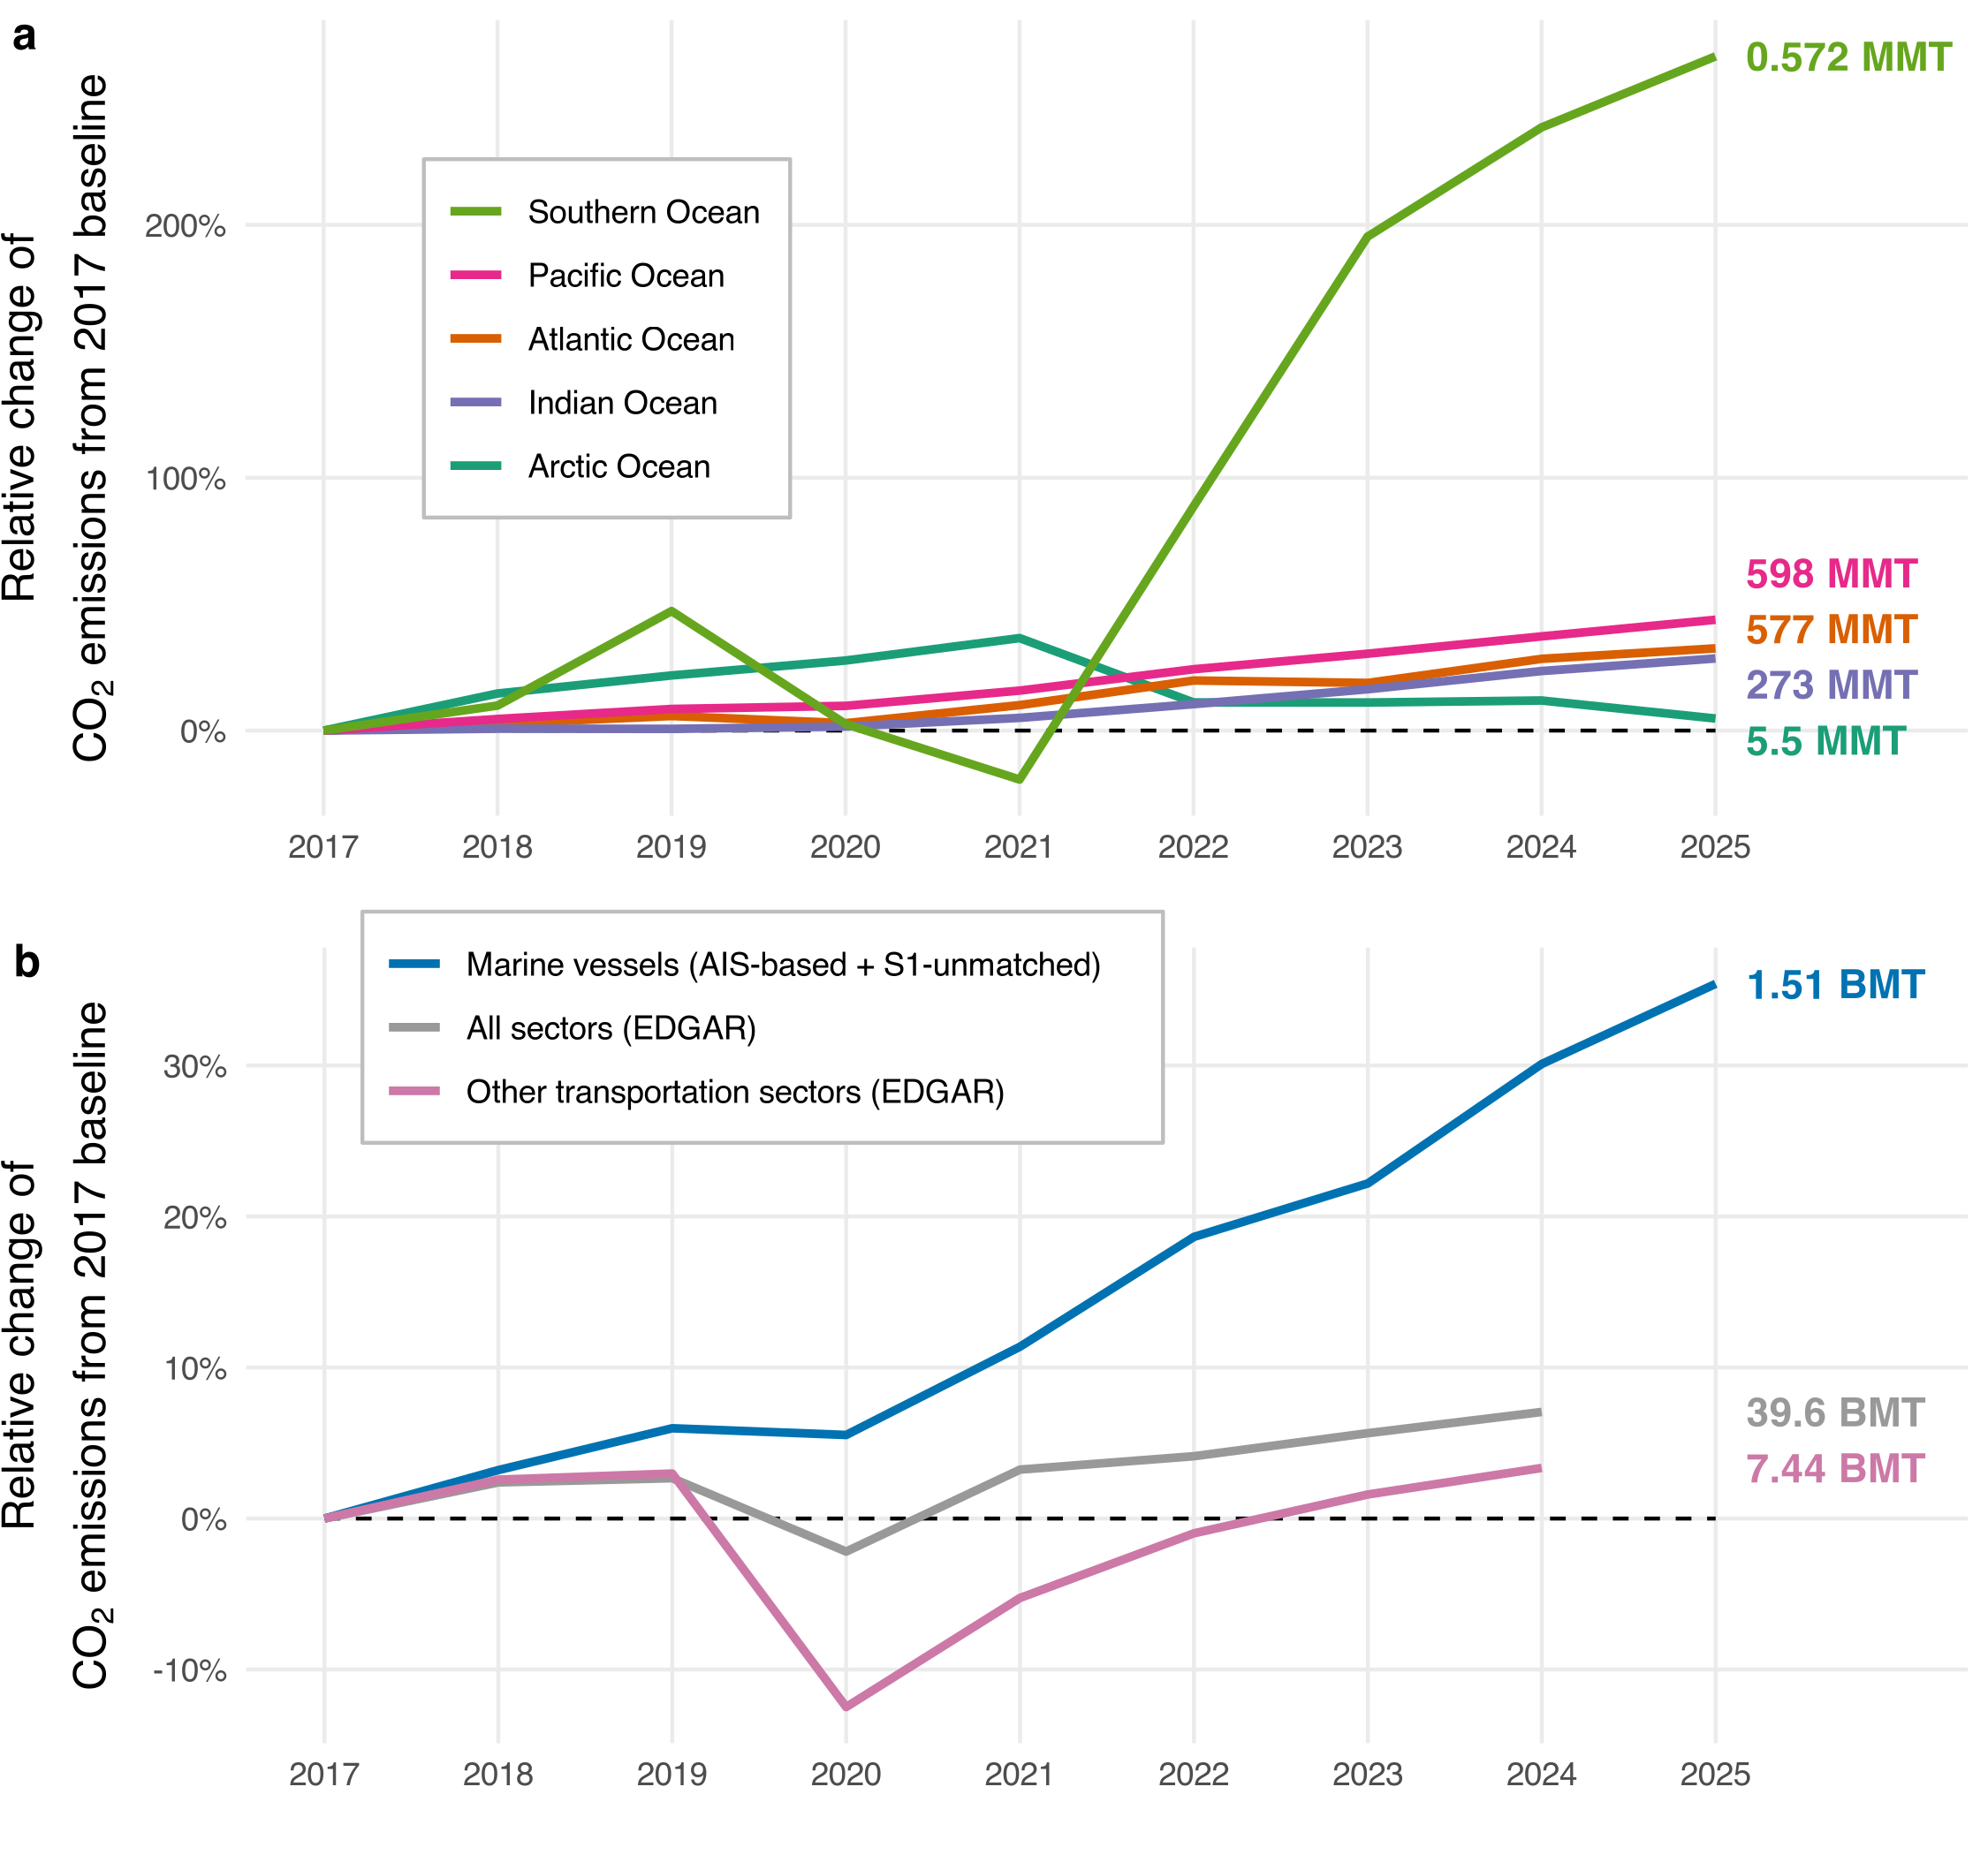
\includegraphics[keepaspectratio]{../figures/fig-emissions-marine-ocean-other-1.png}}

}

\caption{\label{fig-emissions-marine-ocean-other}(A) Trend in CO2
emissions by ocean (normalized to 2017 baesline) . (B) Comparison in
trend of CO2 emissions data (normalized to 2017 baesline) between marine
transportation emissions from GFW, other transportation emissions from
EDGAR, and all sector emissions from EDGAR.}

\end{figure}%

\begin{table}[!h]
\centering
\caption{\label{tab:emissions_by_ocean_summary_tbl}For each ocean, summary of: total 2024 CO$_2$ emissions (metric tonnes); percentage of total 2024 CO$_2$ emissions from across all oceans; and percent change in CO$_2$ emissions from 2017 to 2024.}
\centering
\fontsize{8}{10}\selectfont
\begin{tabular}[t]{l|l|l|l}
\hline
Ocean & CO2 emissions in 2024 (million MT) & Percent of total 2024 CO2 emissions & Percent change in CO2 emissions from 2017 to 2024\\
\hline
indian & 246 & 19.99\% & 24.00\%\\
\hline
southern & 0.607 & 0.05\% & 290.77\%\\
\hline
atlantic & 468 & 38.08\% & 28.74\%\\
\hline
pacific & 510 & 41.49\% & 41.61\%\\
\hline
arctic & 4.76 & 0.39\% & 62.69\%\\
\hline
\end{tabular}
\end{table}

\begin{table}[!h]
\centering
\caption{\label{tab:emissions_by_data_source_summary_tbl}For each data source, summary of: total 2024 CO$_2$ emissions (metric tonnes); and percent change in CO$_2$ emissions from 2017 to 2024.}
\centering
\fontsize{8}{10}\selectfont
\begin{tabular}[t]{l|l|l}
\hline
Data source & CO2 emissions in 2024 (billion MT) & Percent change in CO2 emissions from 2017 to 2024\\
\hline
Other transportation sectors (EDGAR) & 7.44 & 3.35\%\\
\hline
All sectors (EDGAR) & 39.6 & 7.06\%\\
\hline
Marine vessels (AIS + S1) & 1.27 & 32.21\%\\
\hline
\end{tabular}
\end{table}

\section{Supplementary figures}\label{supplementary-figures}

\subsubsection{Relationship between length and engine
power}\label{relationship-between-length-and-engine-power}

\begin{figure}[H]

\centering{

\pandocbounded{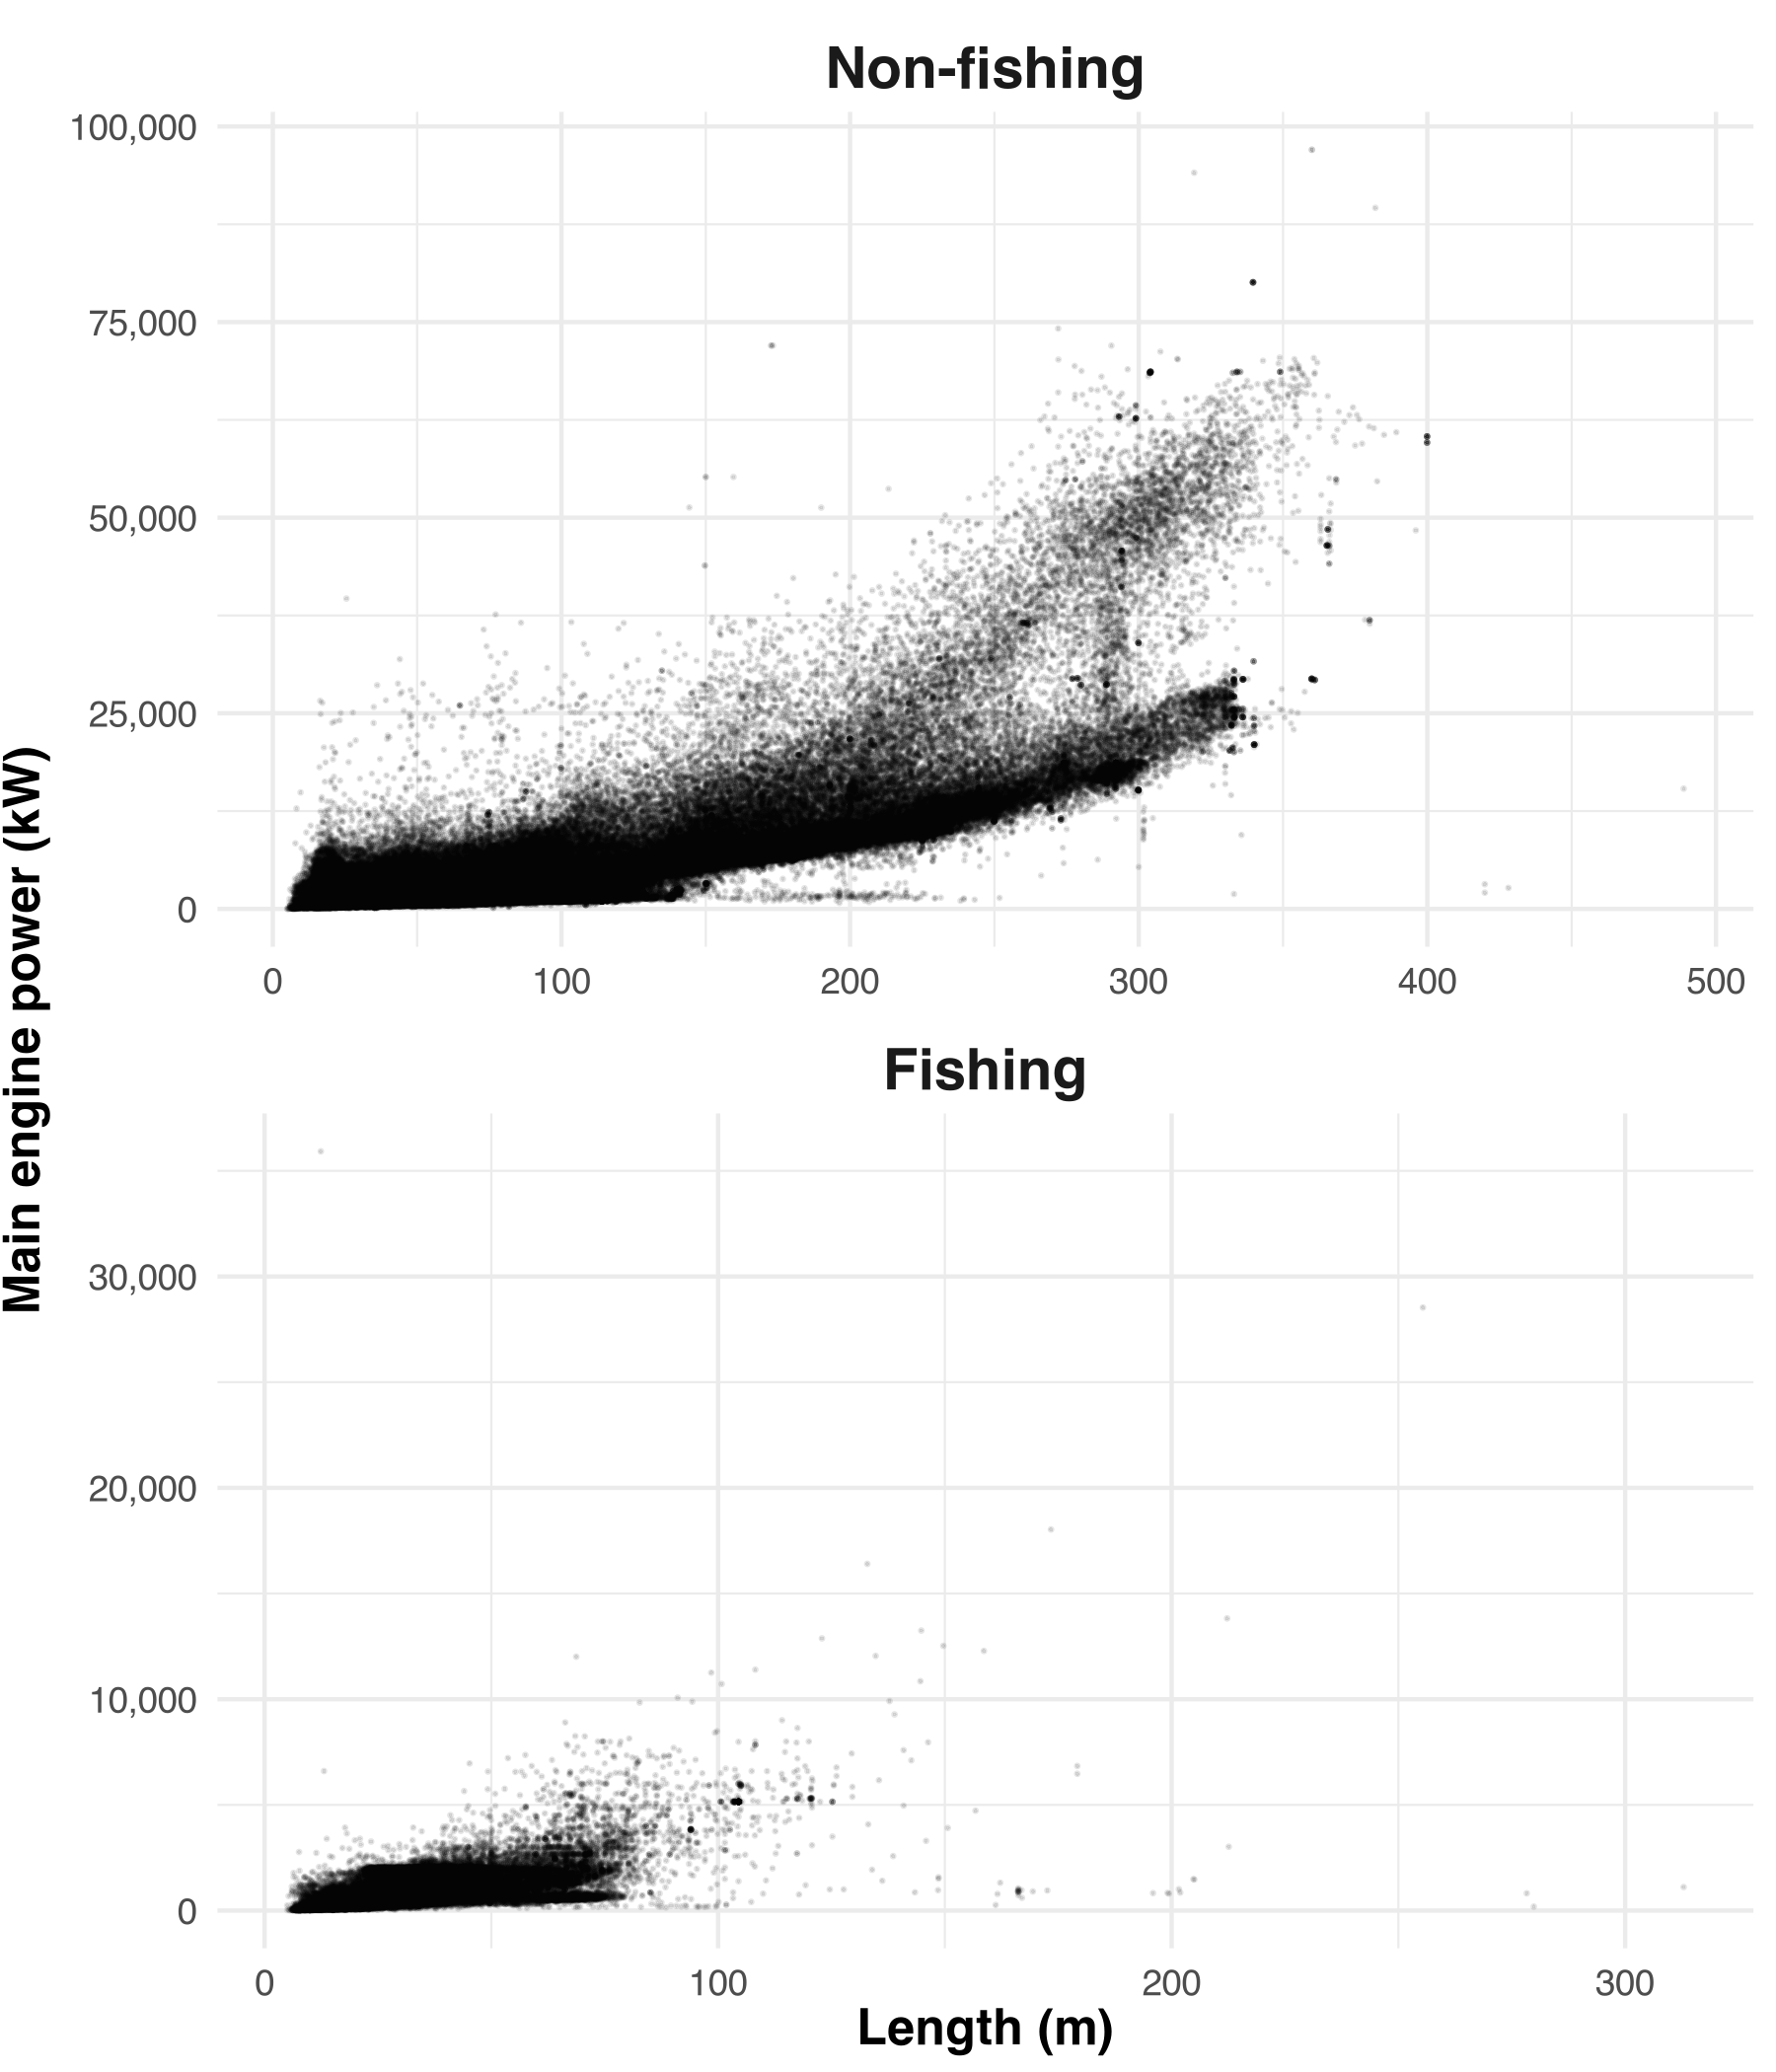
\includegraphics[keepaspectratio]{../figures/fig-ais-length-power-relationship-1.png}}

}

\caption{\label{fig-ais-length-power-relationship}The relationship
between main engine power (kilowatts) and length (meters), where each
point is a specific AIS-broadcasting vessel. The relationship is
disaggregated for non-fishing vessels and fishing vessels.}

\end{figure}%

\subsubsection{Dark fleet emissions, by vessel size and
type}\label{dark-fleet-emissions-by-vessel-size-and-type}

\begin{figure}[H]

\centering{

\pandocbounded{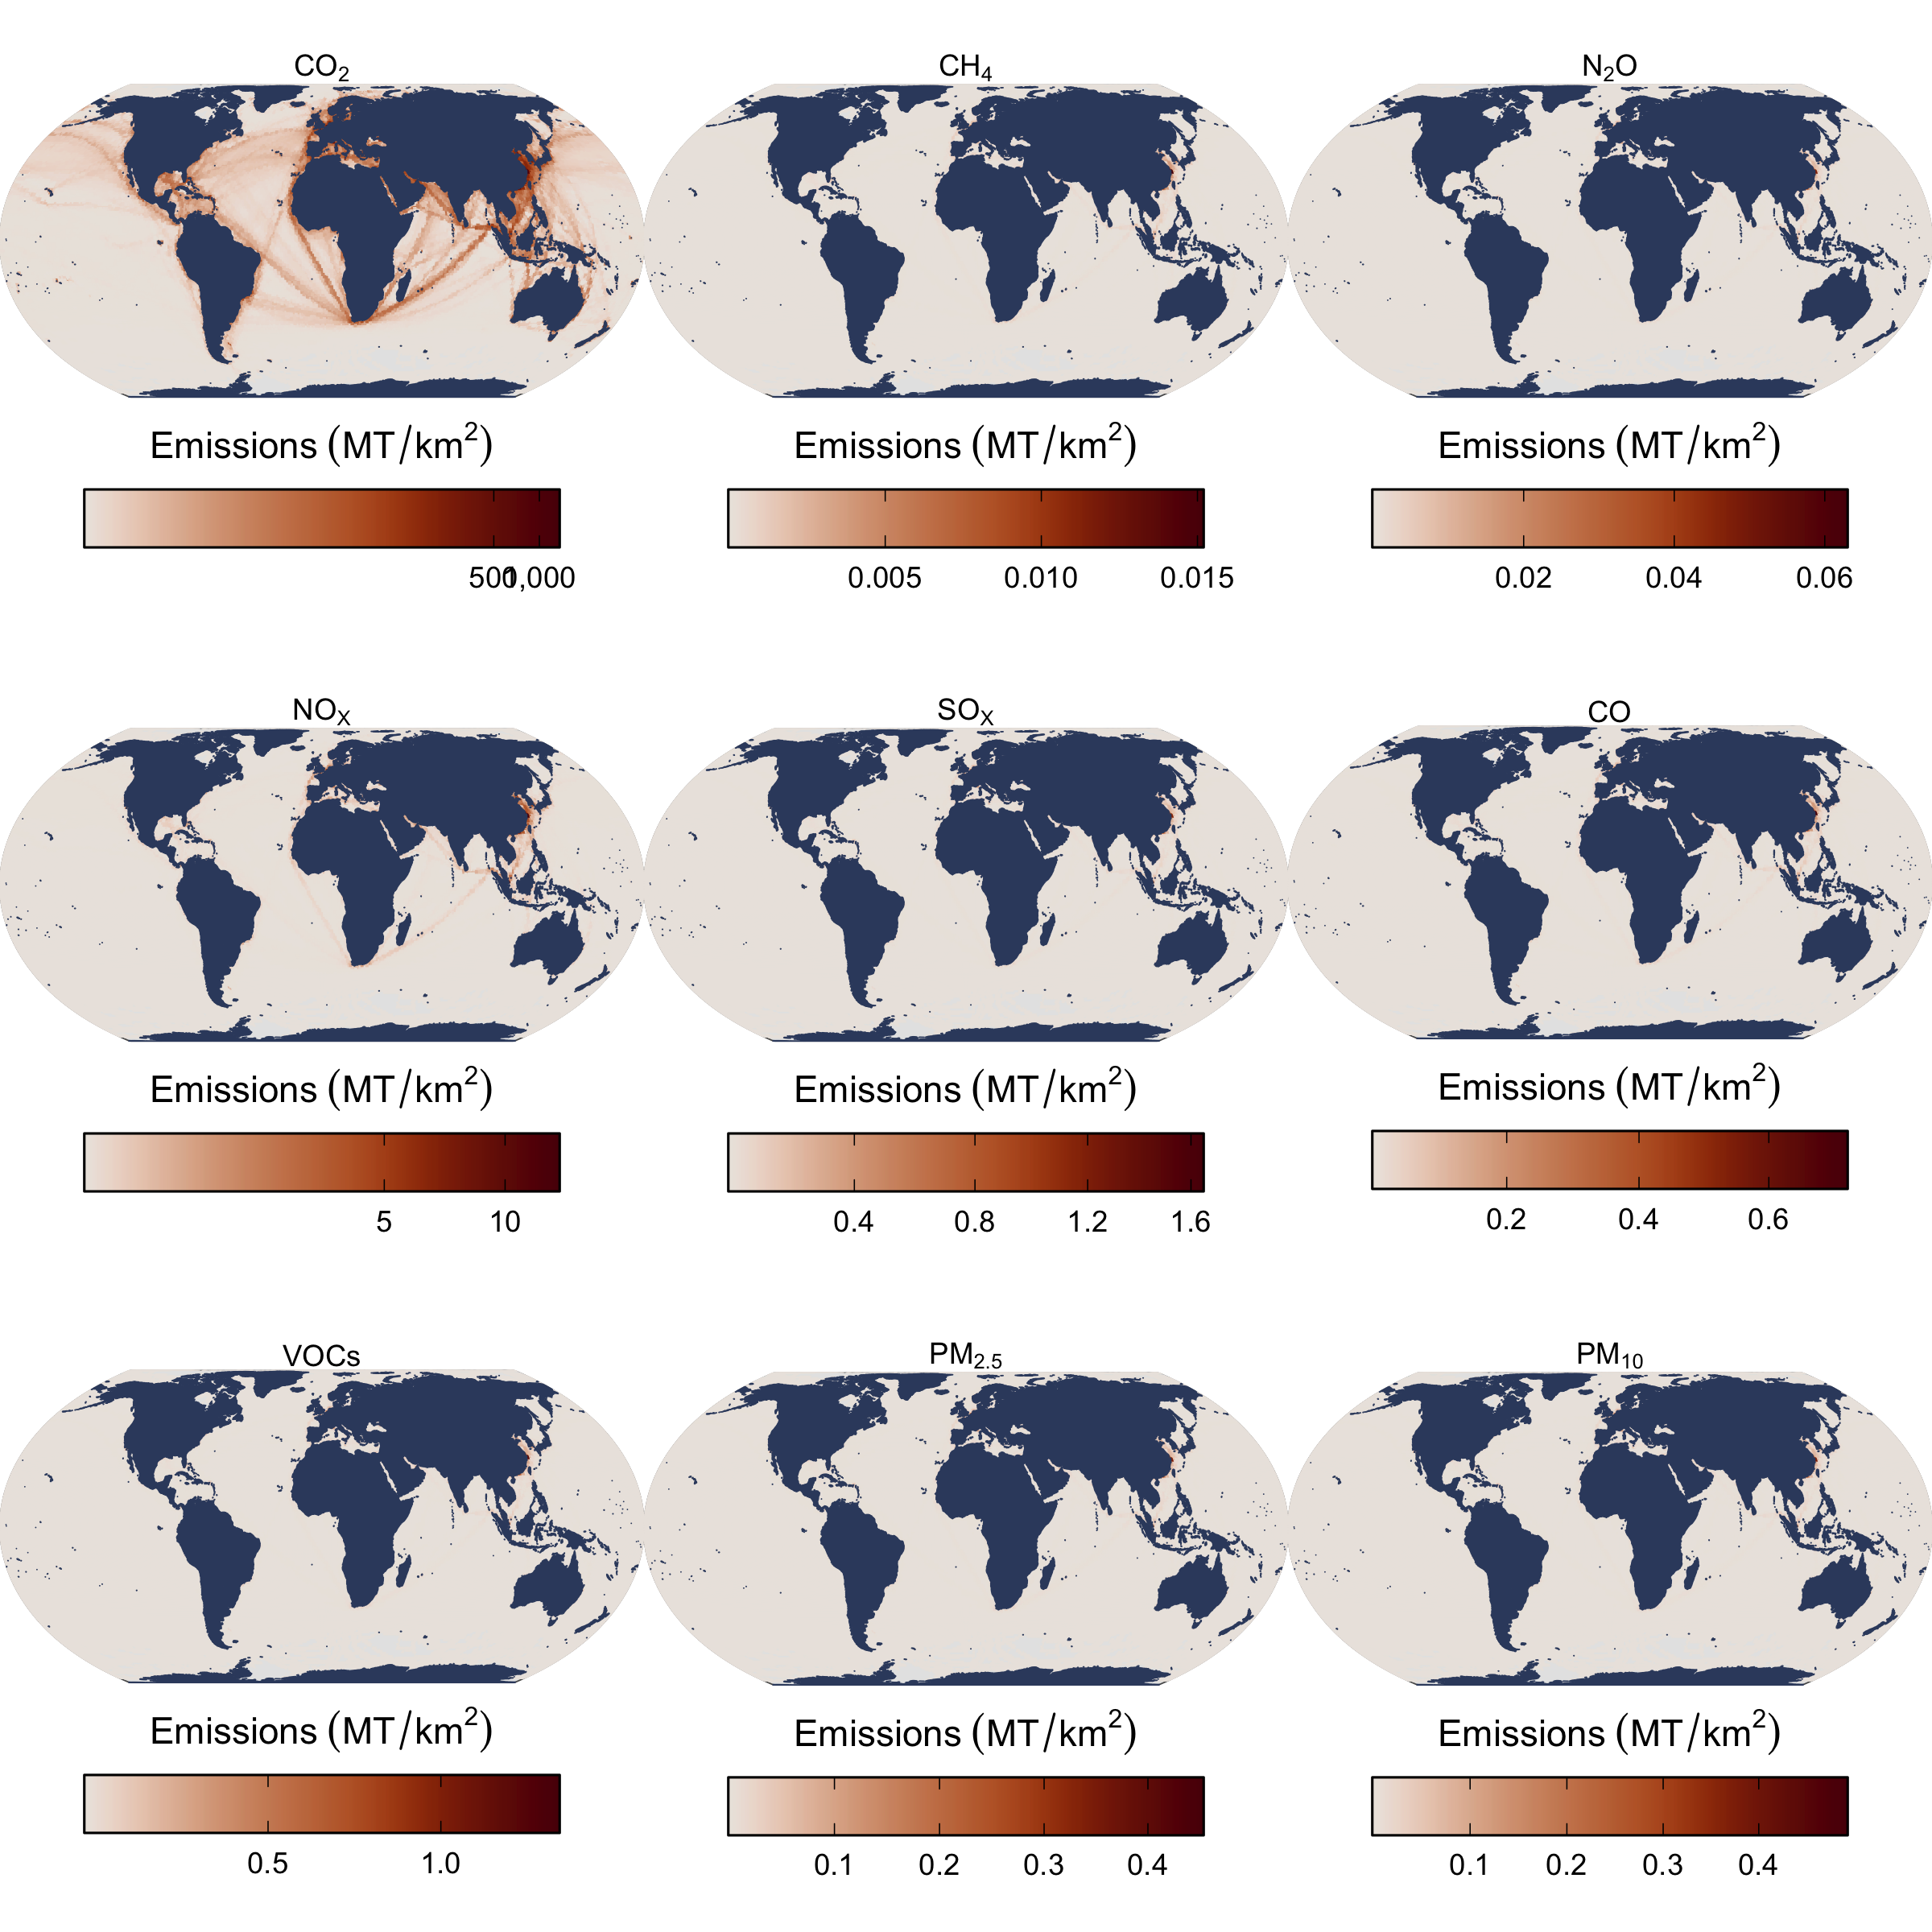
\includegraphics[keepaspectratio]{../figures/fig-pollutant-maps-pseudolog-1.png}}

}

\caption{\label{fig-pollutant-maps-pseudolog}Spatial map of 2024
emissions for each pollutant, aggregated across the AIS-broadcasting
fleet and non-broadcasting, and shown at a 1x1 degree spatial
resolution}

\end{figure}%

\begin{figure}[H]

\centering{

\pandocbounded{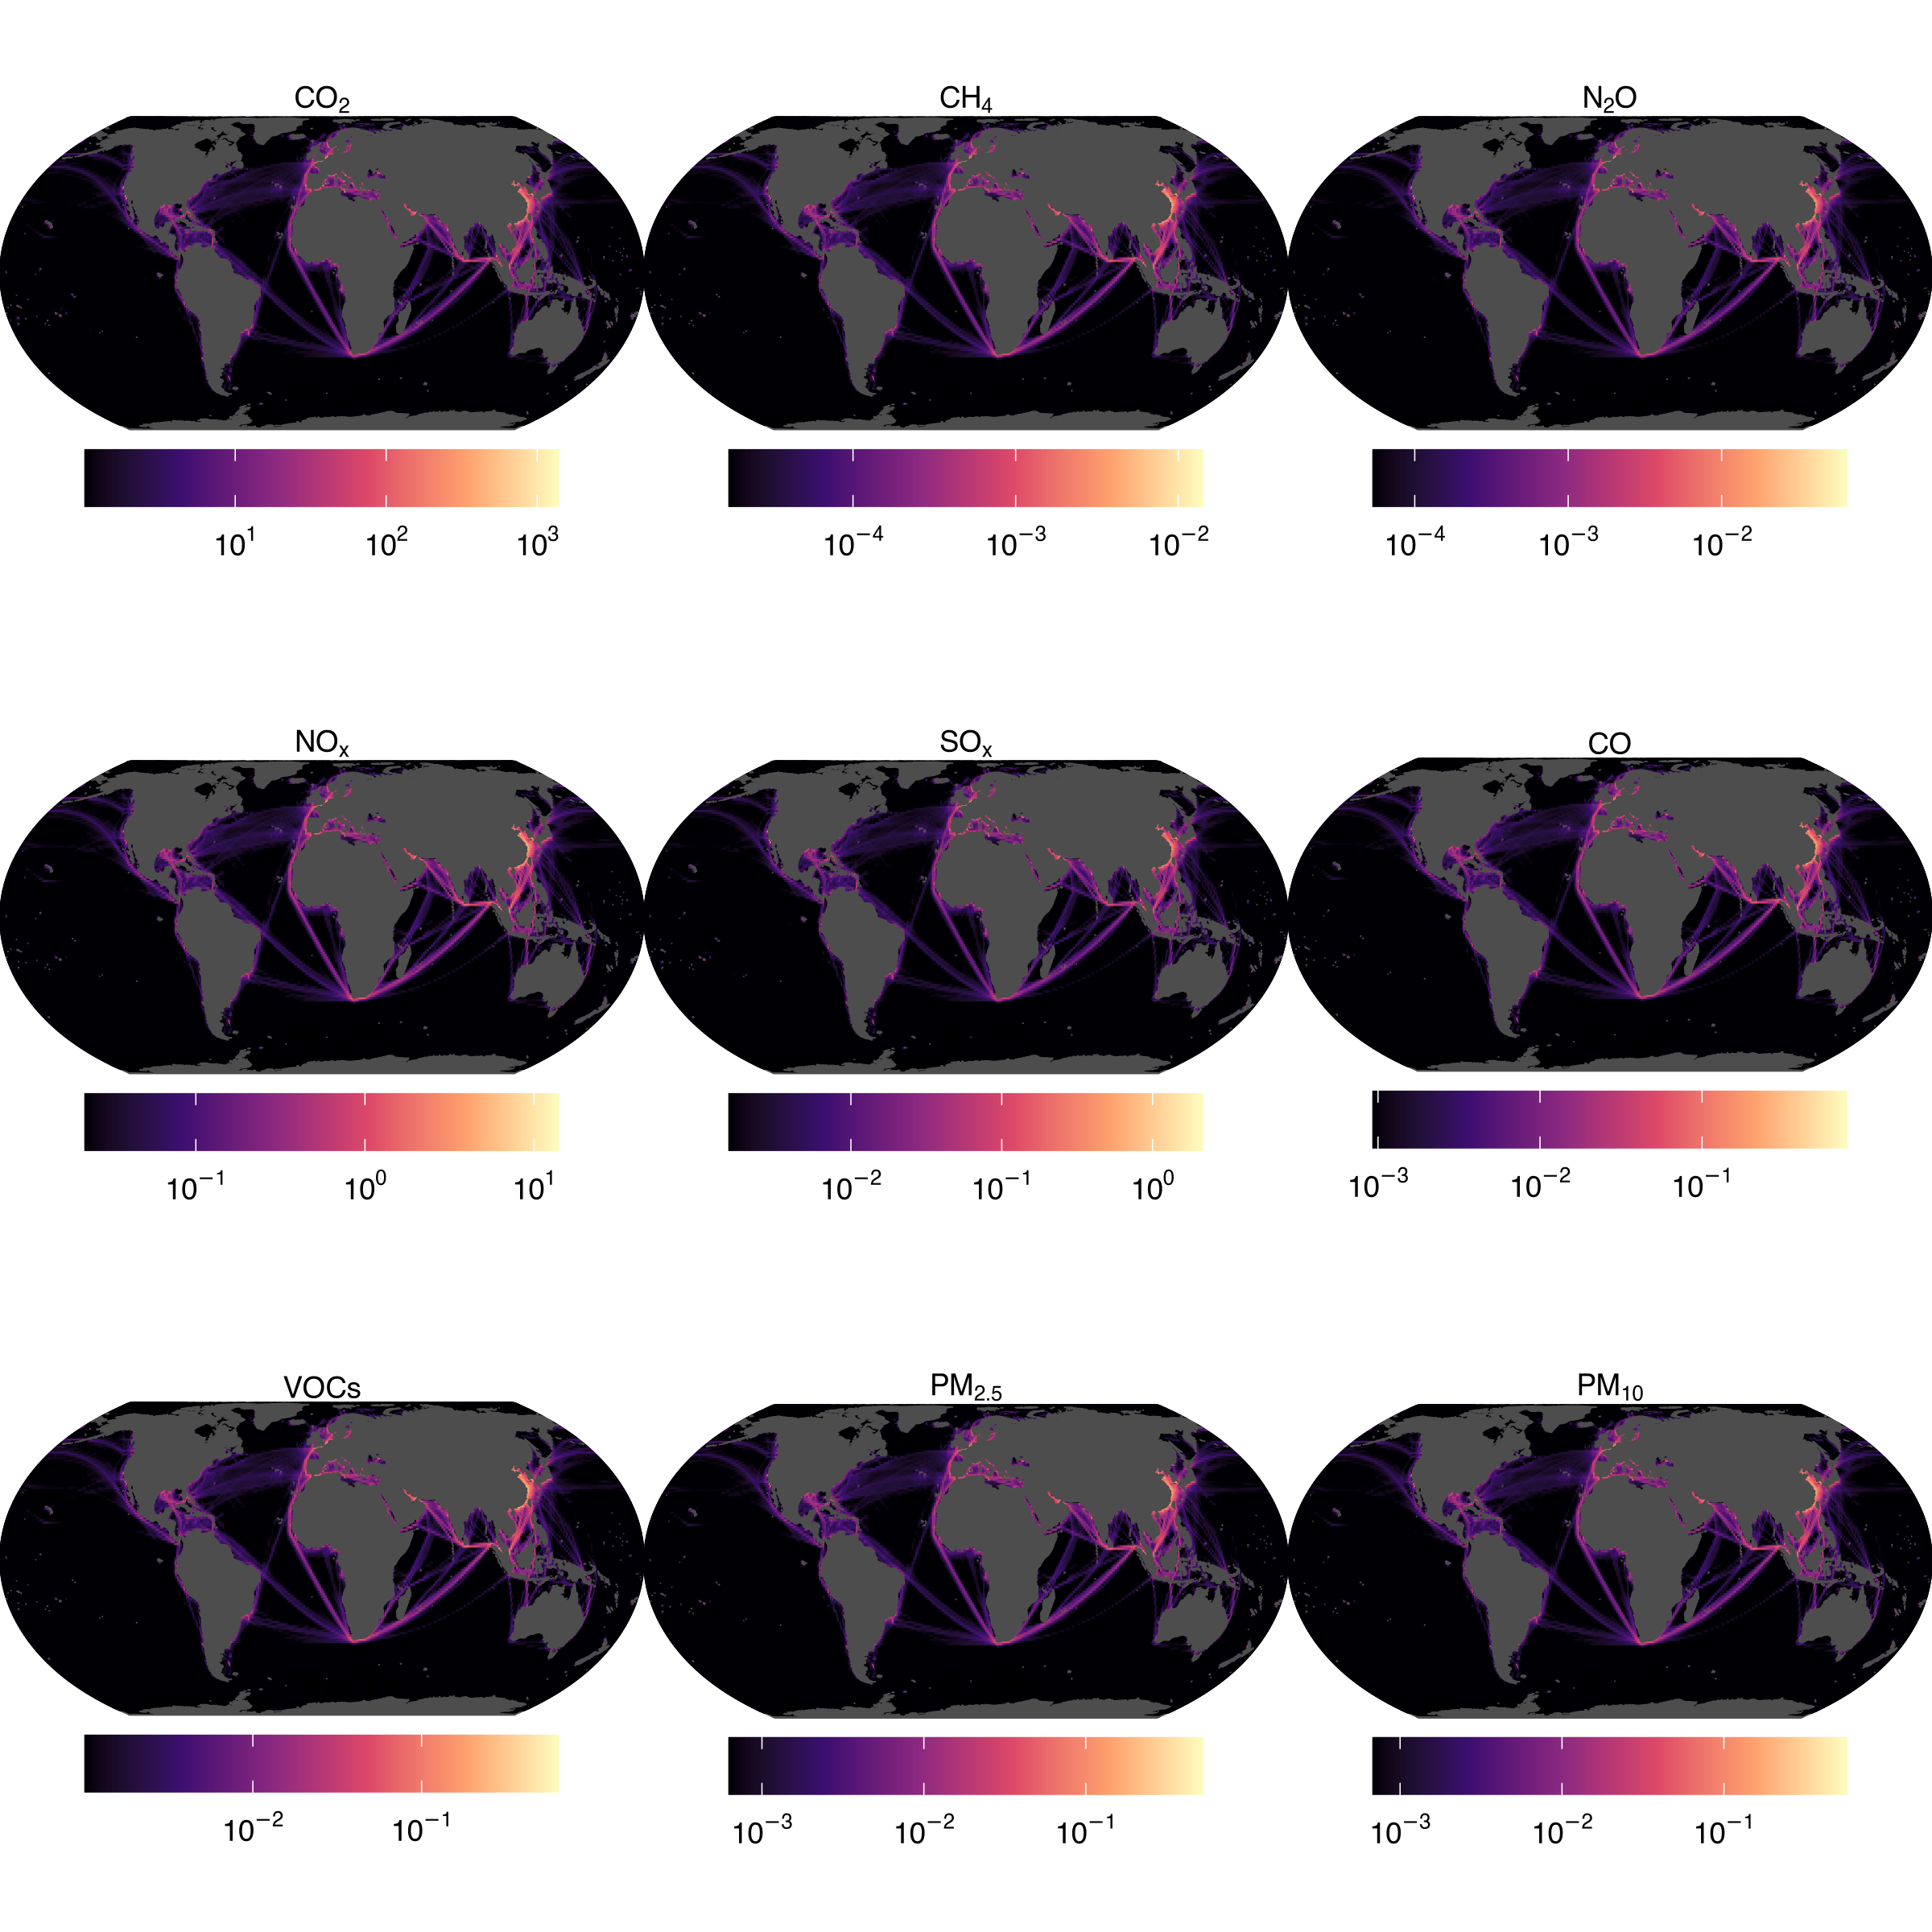
\includegraphics[keepaspectratio]{../figures/fig-pollutant-maps-qlog10-1.png}}

}

\caption{\label{fig-pollutant-maps-qlog10}Spatial map of 2024 emissions
for each pollutant, aggregated across the AIS-broadcasting fleet and
non-broadcasting, and shown at a 1x1 degree spatial resolution. A log-10
scale is applied for visualization to manage the high dynamic range of
emissions. To ensure visual clarity and suppress background noise, the
bottom 1\% of the emission distribution has been excluded from the color
mapping.}

\end{figure}%

\begin{figure}[H]

\centering{

\pandocbounded{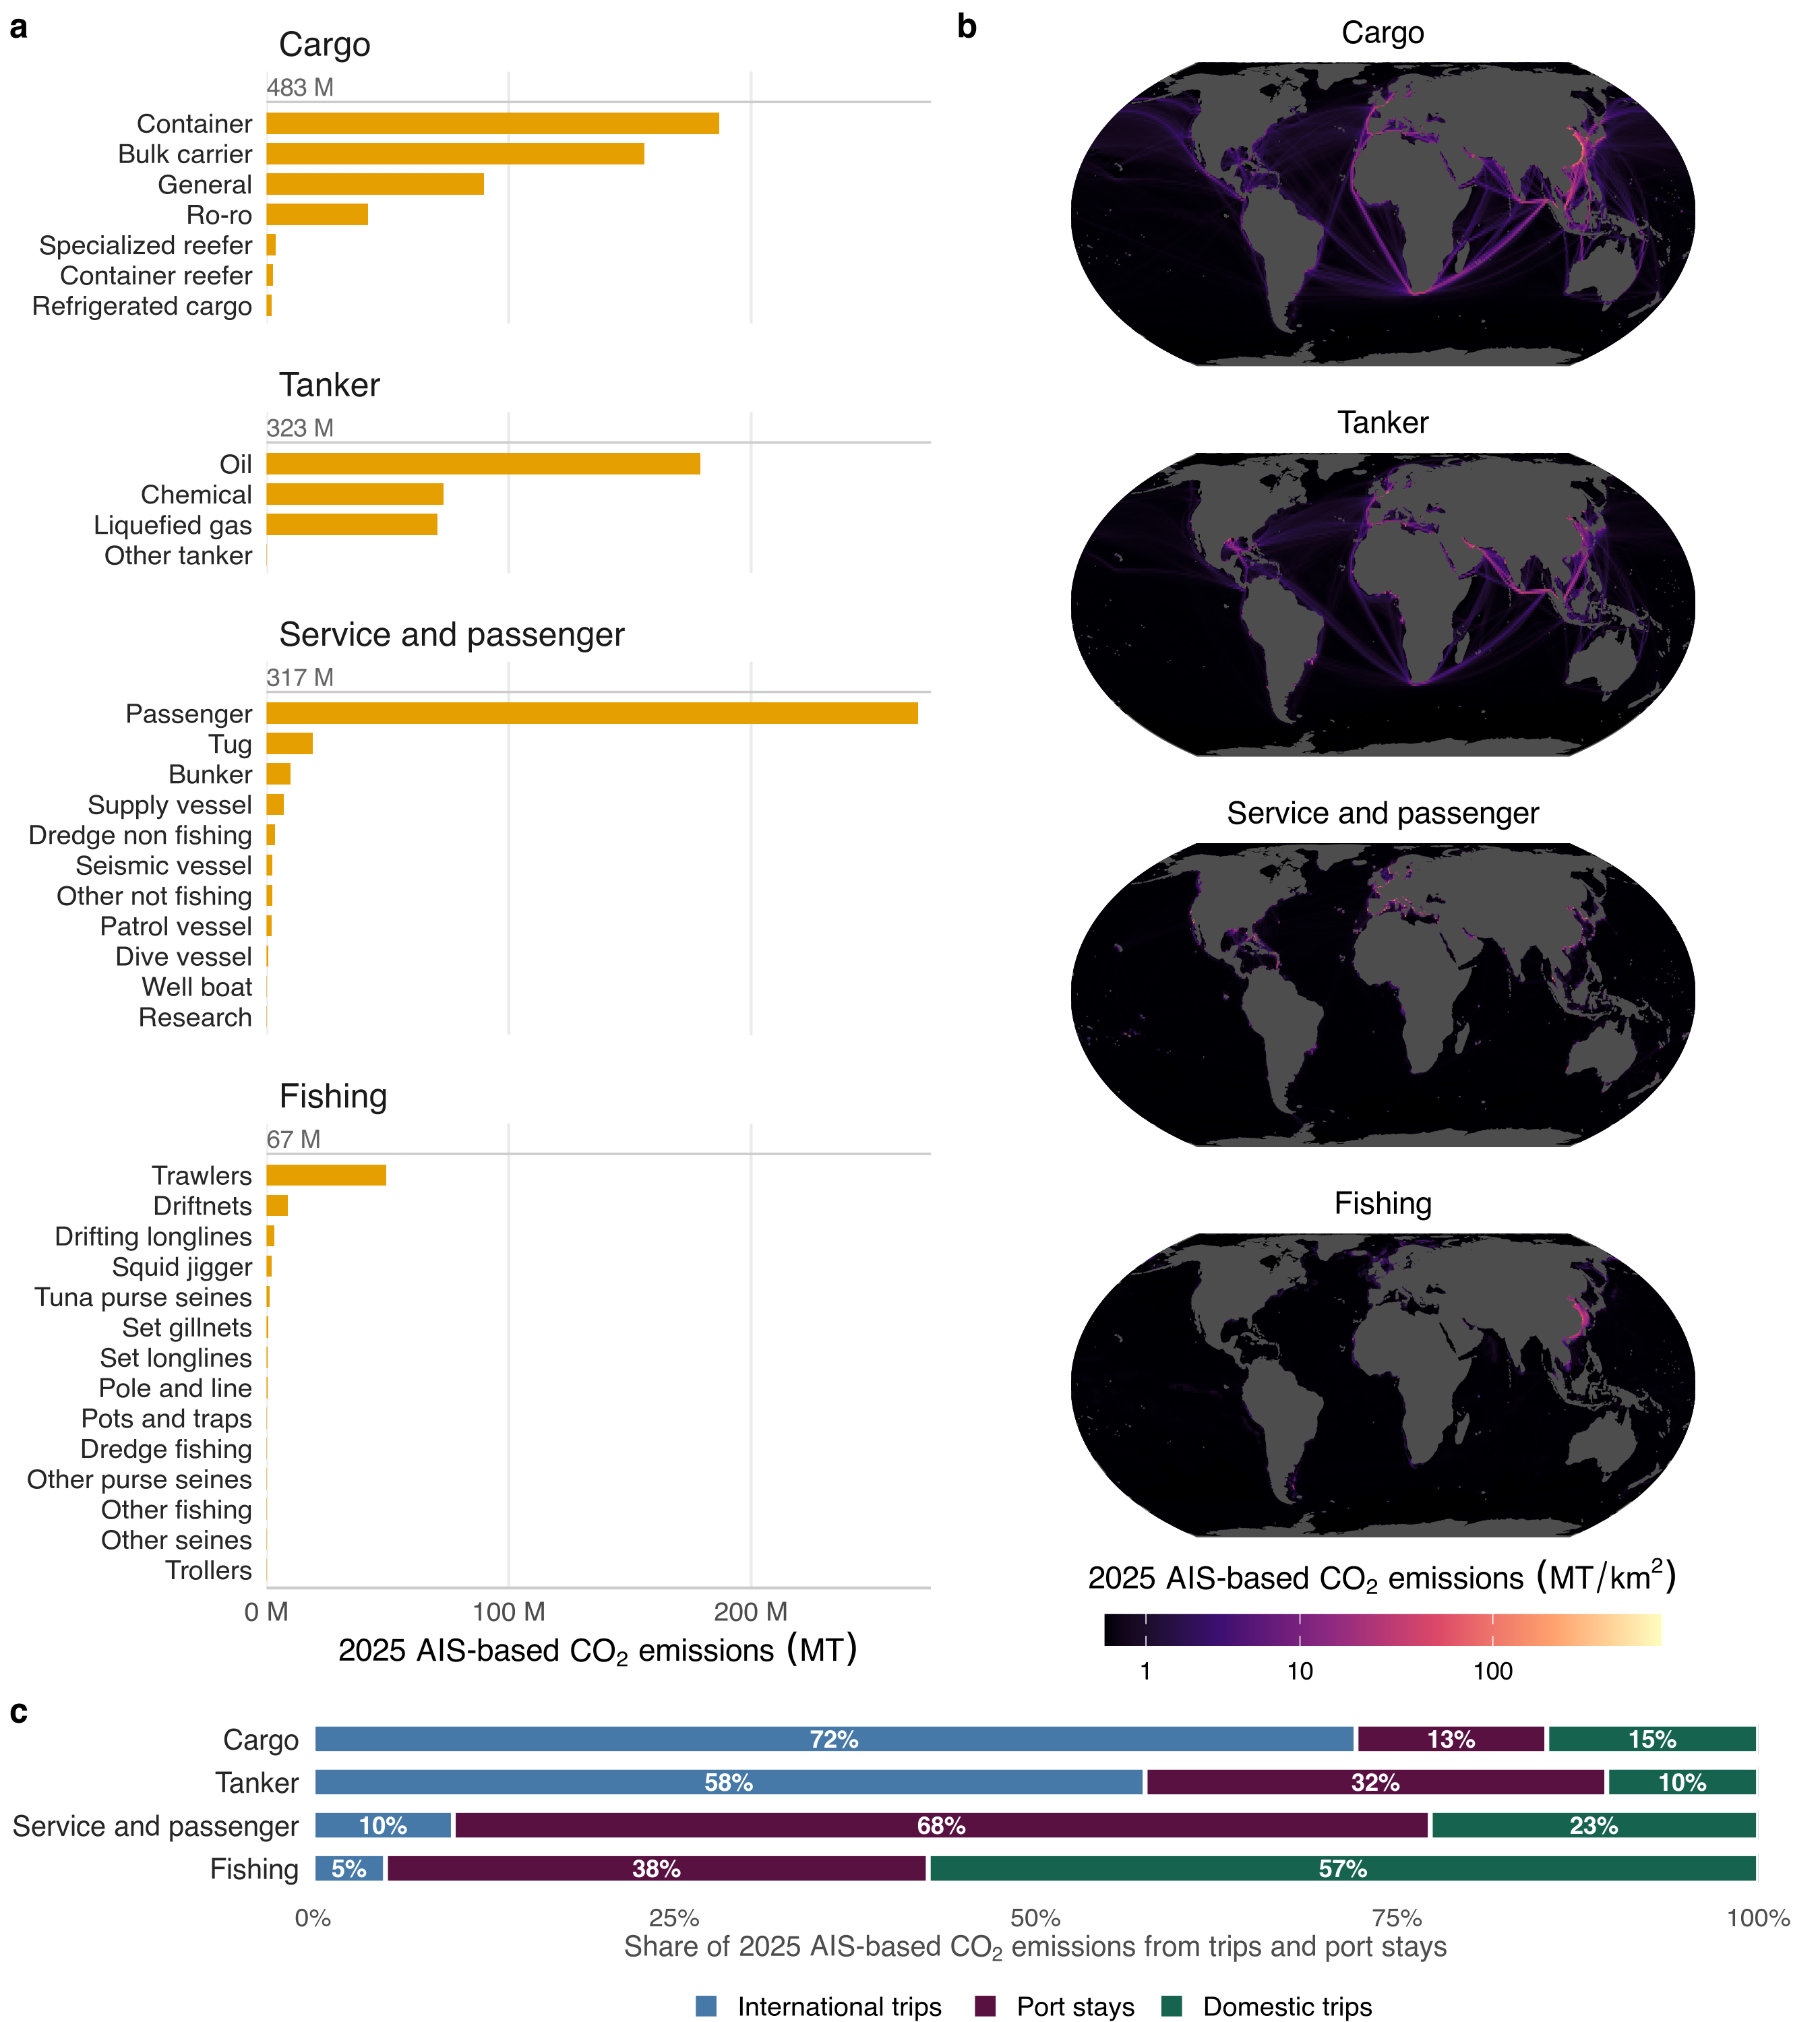
\includegraphics[keepaspectratio]{../figures/fig-ais-data-richness-1.png}}

}

\caption{\label{fig-ais-data-richness}(A) 2024 CO\(_{2}\) emissions by
vessel type for AIS-broadcasting vessels. (B) 2024 CO\(_{2}\) emissions
by country for AIS-broadcasting vessels during domestic trips,
international trips (where emissions of each trip are partitioned
equally to its departure and arrival country), and during port stays.
Countries with no values are shown in black.}

\end{figure}%

\section{Figure 3.1 -----}\label{figure-3.1}

\paragraph{Spatial emissions by fleet
(annual)}\label{spatial-emissions-by-fleet-annual}

\begin{figure}[H]

\centering{

\pandocbounded{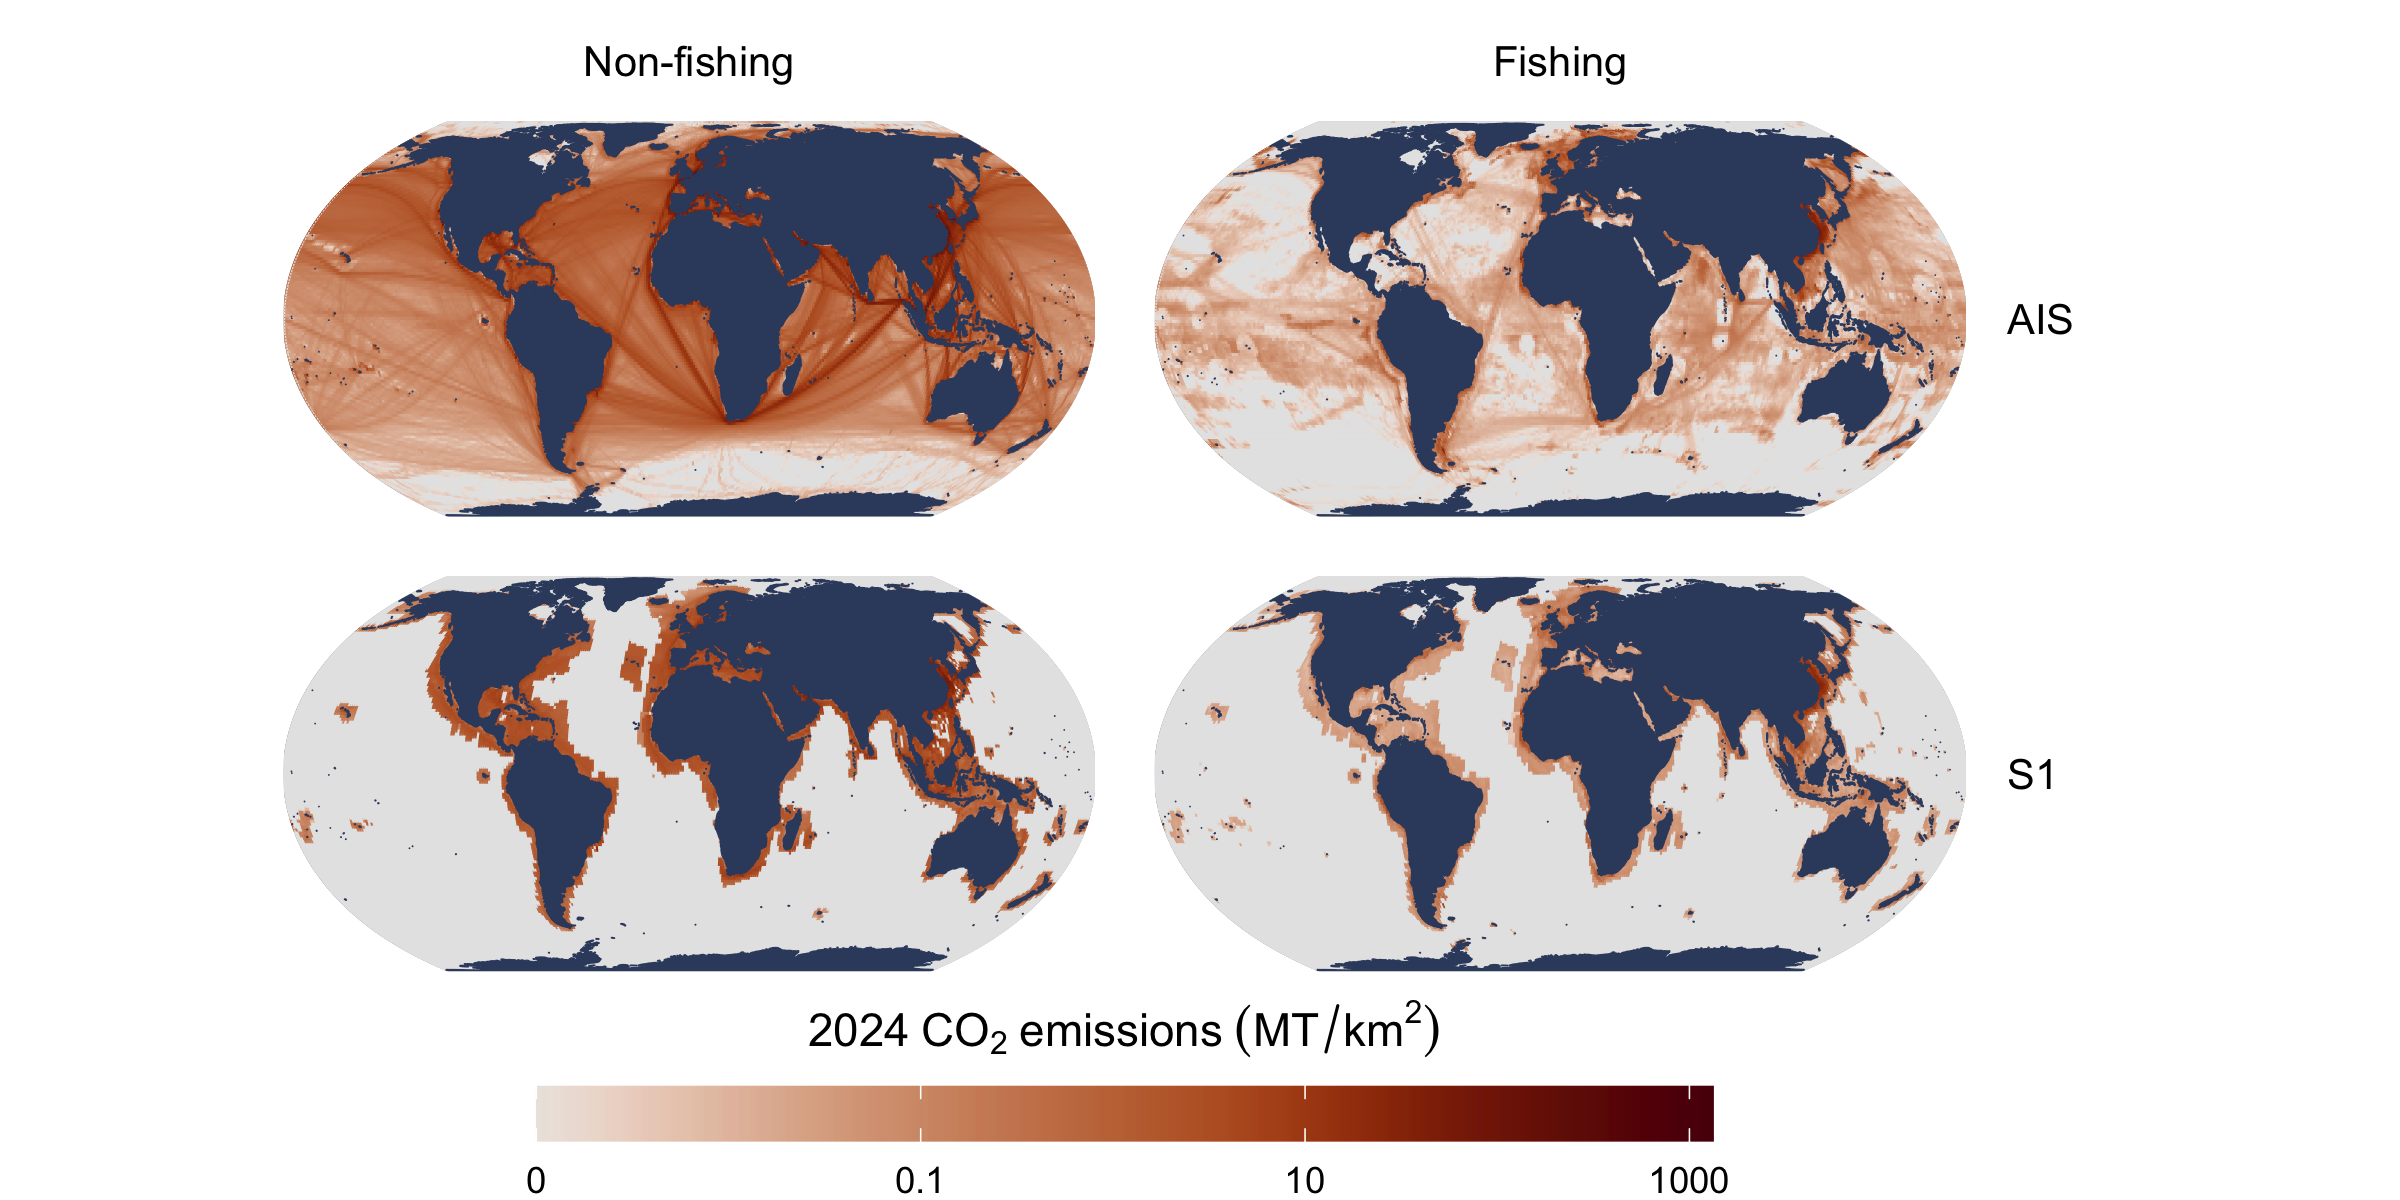
\includegraphics[keepaspectratio]{../figures/fig-spatial-emissions-by-fleet-2024-1.png}}

}

\caption{\label{fig-spatial-emissions-by-fleet-2024}Spatial distribution
of cumulative CO\(_{2}\) emissions (Mt/km2) for AIS/S1, and
fishing/non-fishing fleets, from 2017 to 2024, in MT/Km\(^{2}\)}

\end{figure}%

\paragraph{Spatial emissions by fleet
(total)}\label{spatial-emissions-by-fleet-total}

\begin{figure}[H]

\centering{

\pandocbounded{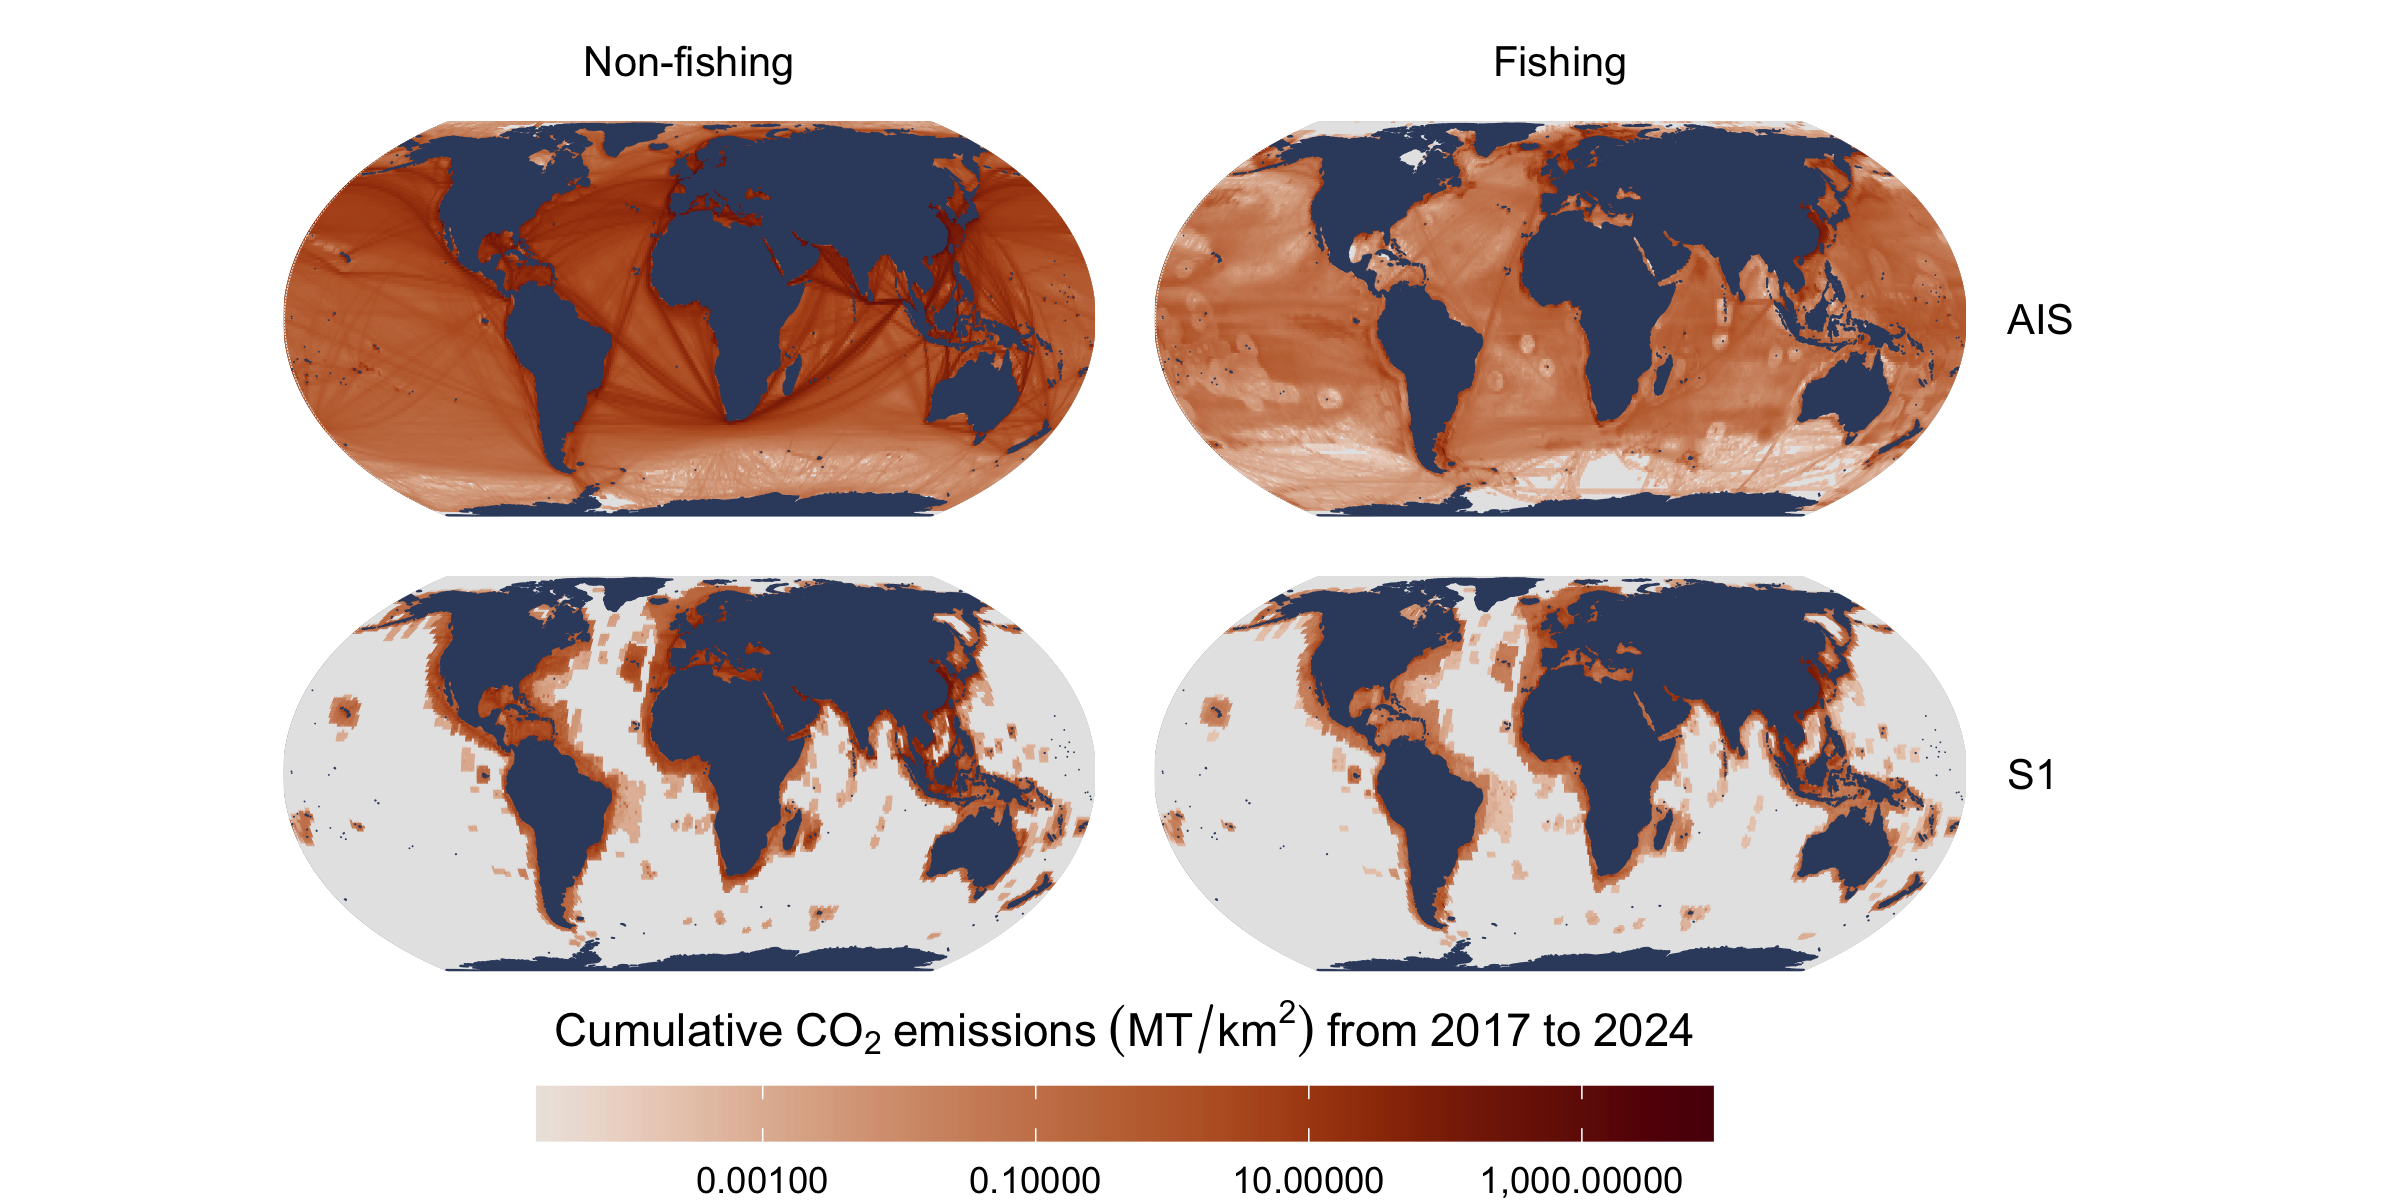
\includegraphics[keepaspectratio]{../figures/fig-spatial-emissions-by-fleet-total-qlog10-1.png}}

}

\caption{\label{fig-spatial-emissions-by-fleet-total-qlog10}Spatial
distribution of cumulative CO\(_{2}\) emissions (Mt/km2) for AIS/S1, and
fishing/non-fishing fleets, from 2017 to 2024, in
MT/Km\(^{2}. A log-10 scale is applied for visualization to manage the high dynamic range of emissions. To ensure visual clarity and suppress background noise, the bottom 1% of the emission distribution has been excluded from the color mapping.
\)}

\end{figure}%

\begin{figure}[H]

\centering{

\pandocbounded{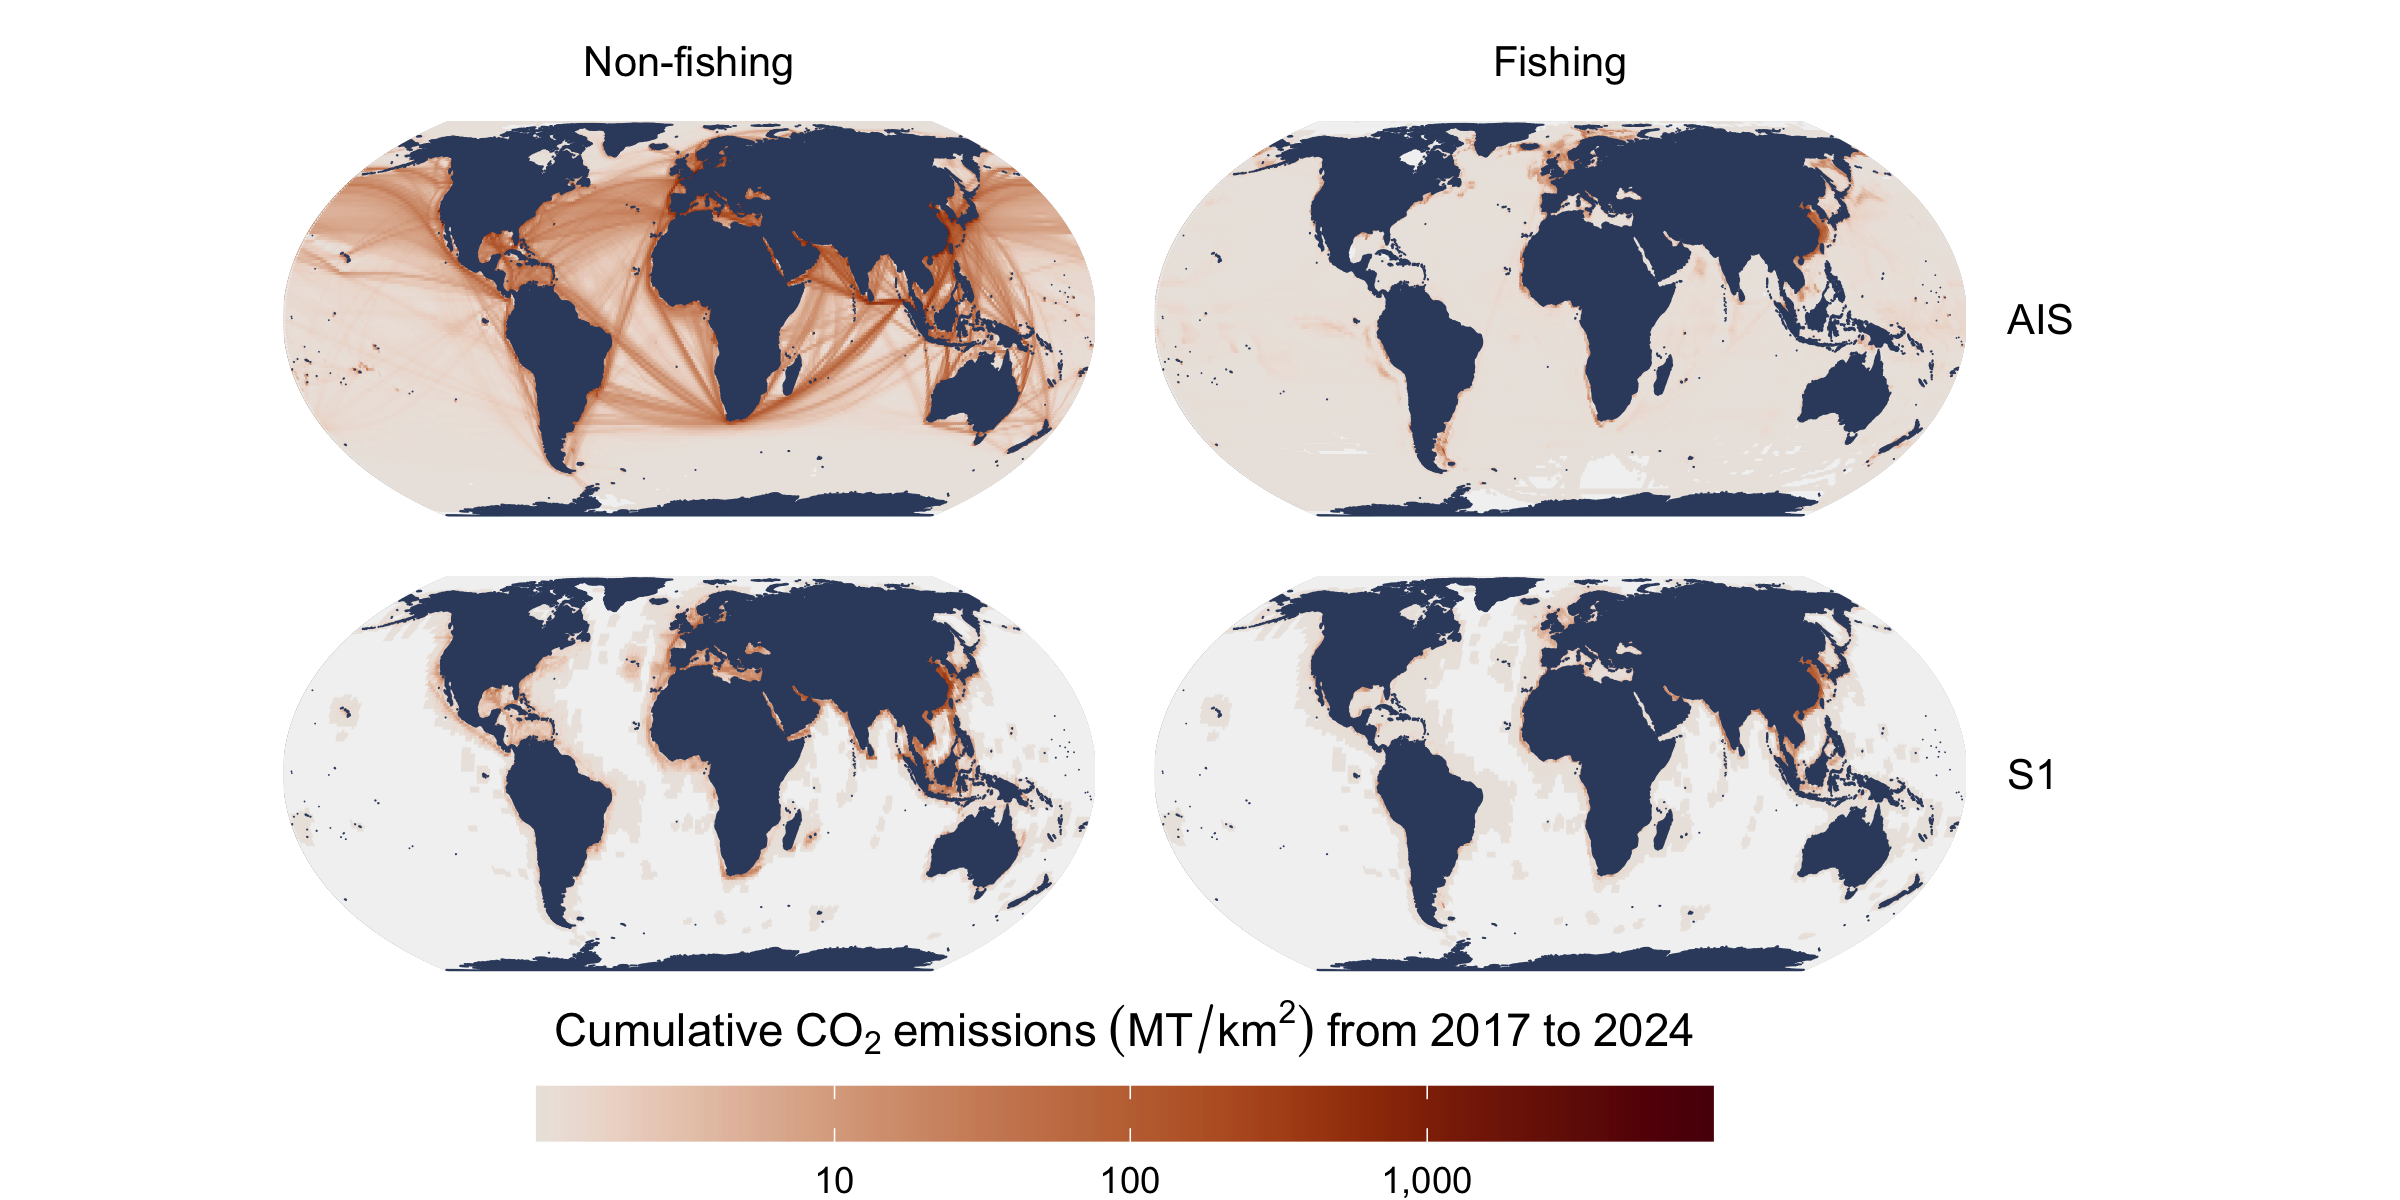
\includegraphics[keepaspectratio]{../figures/fig-spatial-emissions-by-fleet-total-pseudolog-1.png}}

}

\caption{\label{fig-spatial-emissions-by-fleet-total-pseudolog}Spatial
distribution of cumulative CO\(_{2}\) emissions (Mt/km2) for AIS/S1, and
fishing/non-fishing fleets, from 2017 to 2024, in
MT/Km\(^{2}. A pseudolog-10 scale is applied for visualization to manage the high dynamic range of emissions, suppressing near-zero values while preserving emission hotspots.\)}

\end{figure}%

\begin{figure}[H]

\centering{

\pandocbounded{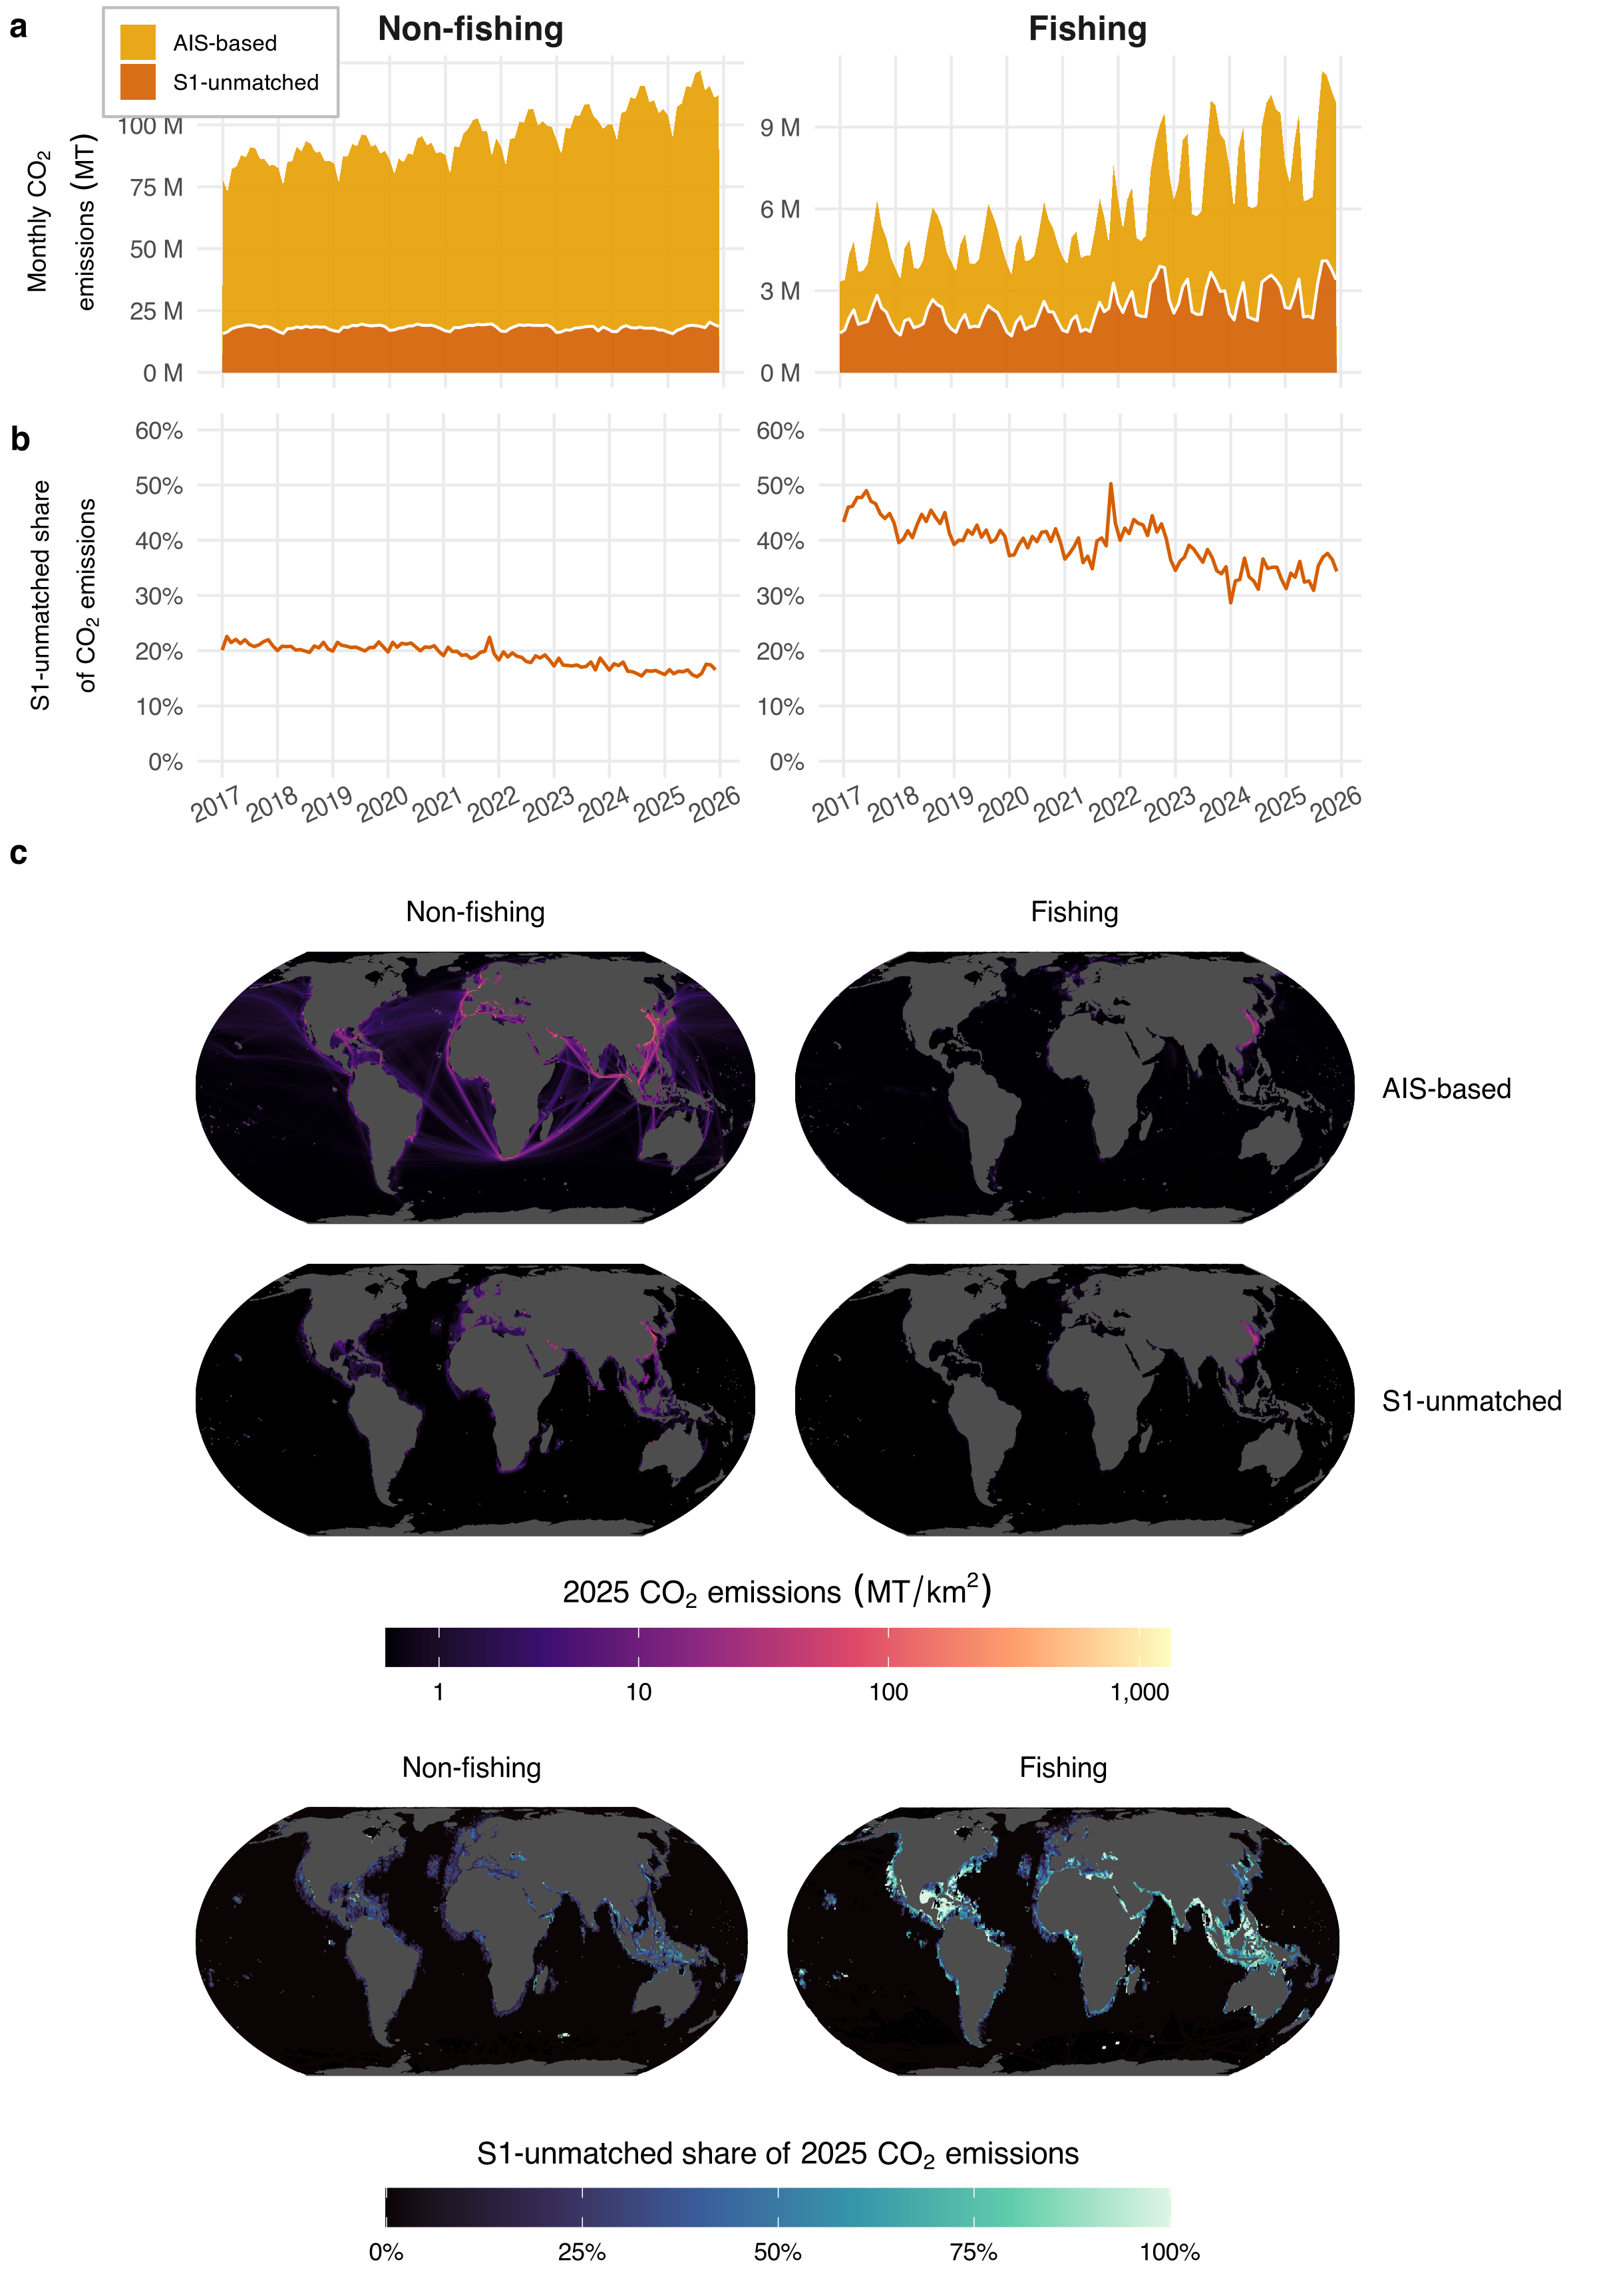
\includegraphics[keepaspectratio]{../figures/fig-spatial-temporal-richness-by-fleet-total-pseudolog-1.png}}

}

\caption{\label{fig-spatial-temporal-richness-by-fleet-total-pseudolog}(A)
Time series of monthly global CO\(_2\) emissions, aggregated across
AIS-broadcasting and non-broadcasting fleets, for both fishing and
non-fishing boats. (B) Spatial distribution of cumulative CO\(_{2}\)
emissions (Mt/km2) for AIS/S1, and fishing/non-fishing fleets, from 2017
to 2024, in
MT/Km\(^{2}. A pseudolog-10 scale is applied for visualization to manage the high dynamic range of emissions, suppressing near-zero values while preserving emission hotspots.\)}

\end{figure}%

\subsubsection{Other plots}\label{other-plots}

\begin{longtable}[]{@{}lrll@{}}

\caption{\label{tbl-top-port-stay-emissions-by-country}Top 10 countries
in terms of 2024 port stay emissions.}

\tabularnewline

\toprule\noalign{}
country\_iso3 & emissions\_co2\_mt & type & country \\
\midrule\noalign{}
\endhead
\bottomrule\noalign{}
\endlastfoot
CHN & 51854306 & Domestic trips & China \\
JPN & 13072972 & Domestic trips & Japan \\
USA & 12891805 & Domestic trips & United States \\
CHN & 79738790 & International trips & China \\
MYS & 48225876 & International trips & Malaysia \\
USA & 46681429 & International trips & United States \\
CHN & 43714734 & Port stays & China \\
USA & 19099768 & Port stays & United States \\
IDN & 7449759 & Port stays & Indonesia \\

\end{longtable}

\begin{figure}[H]

\centering{

\pandocbounded{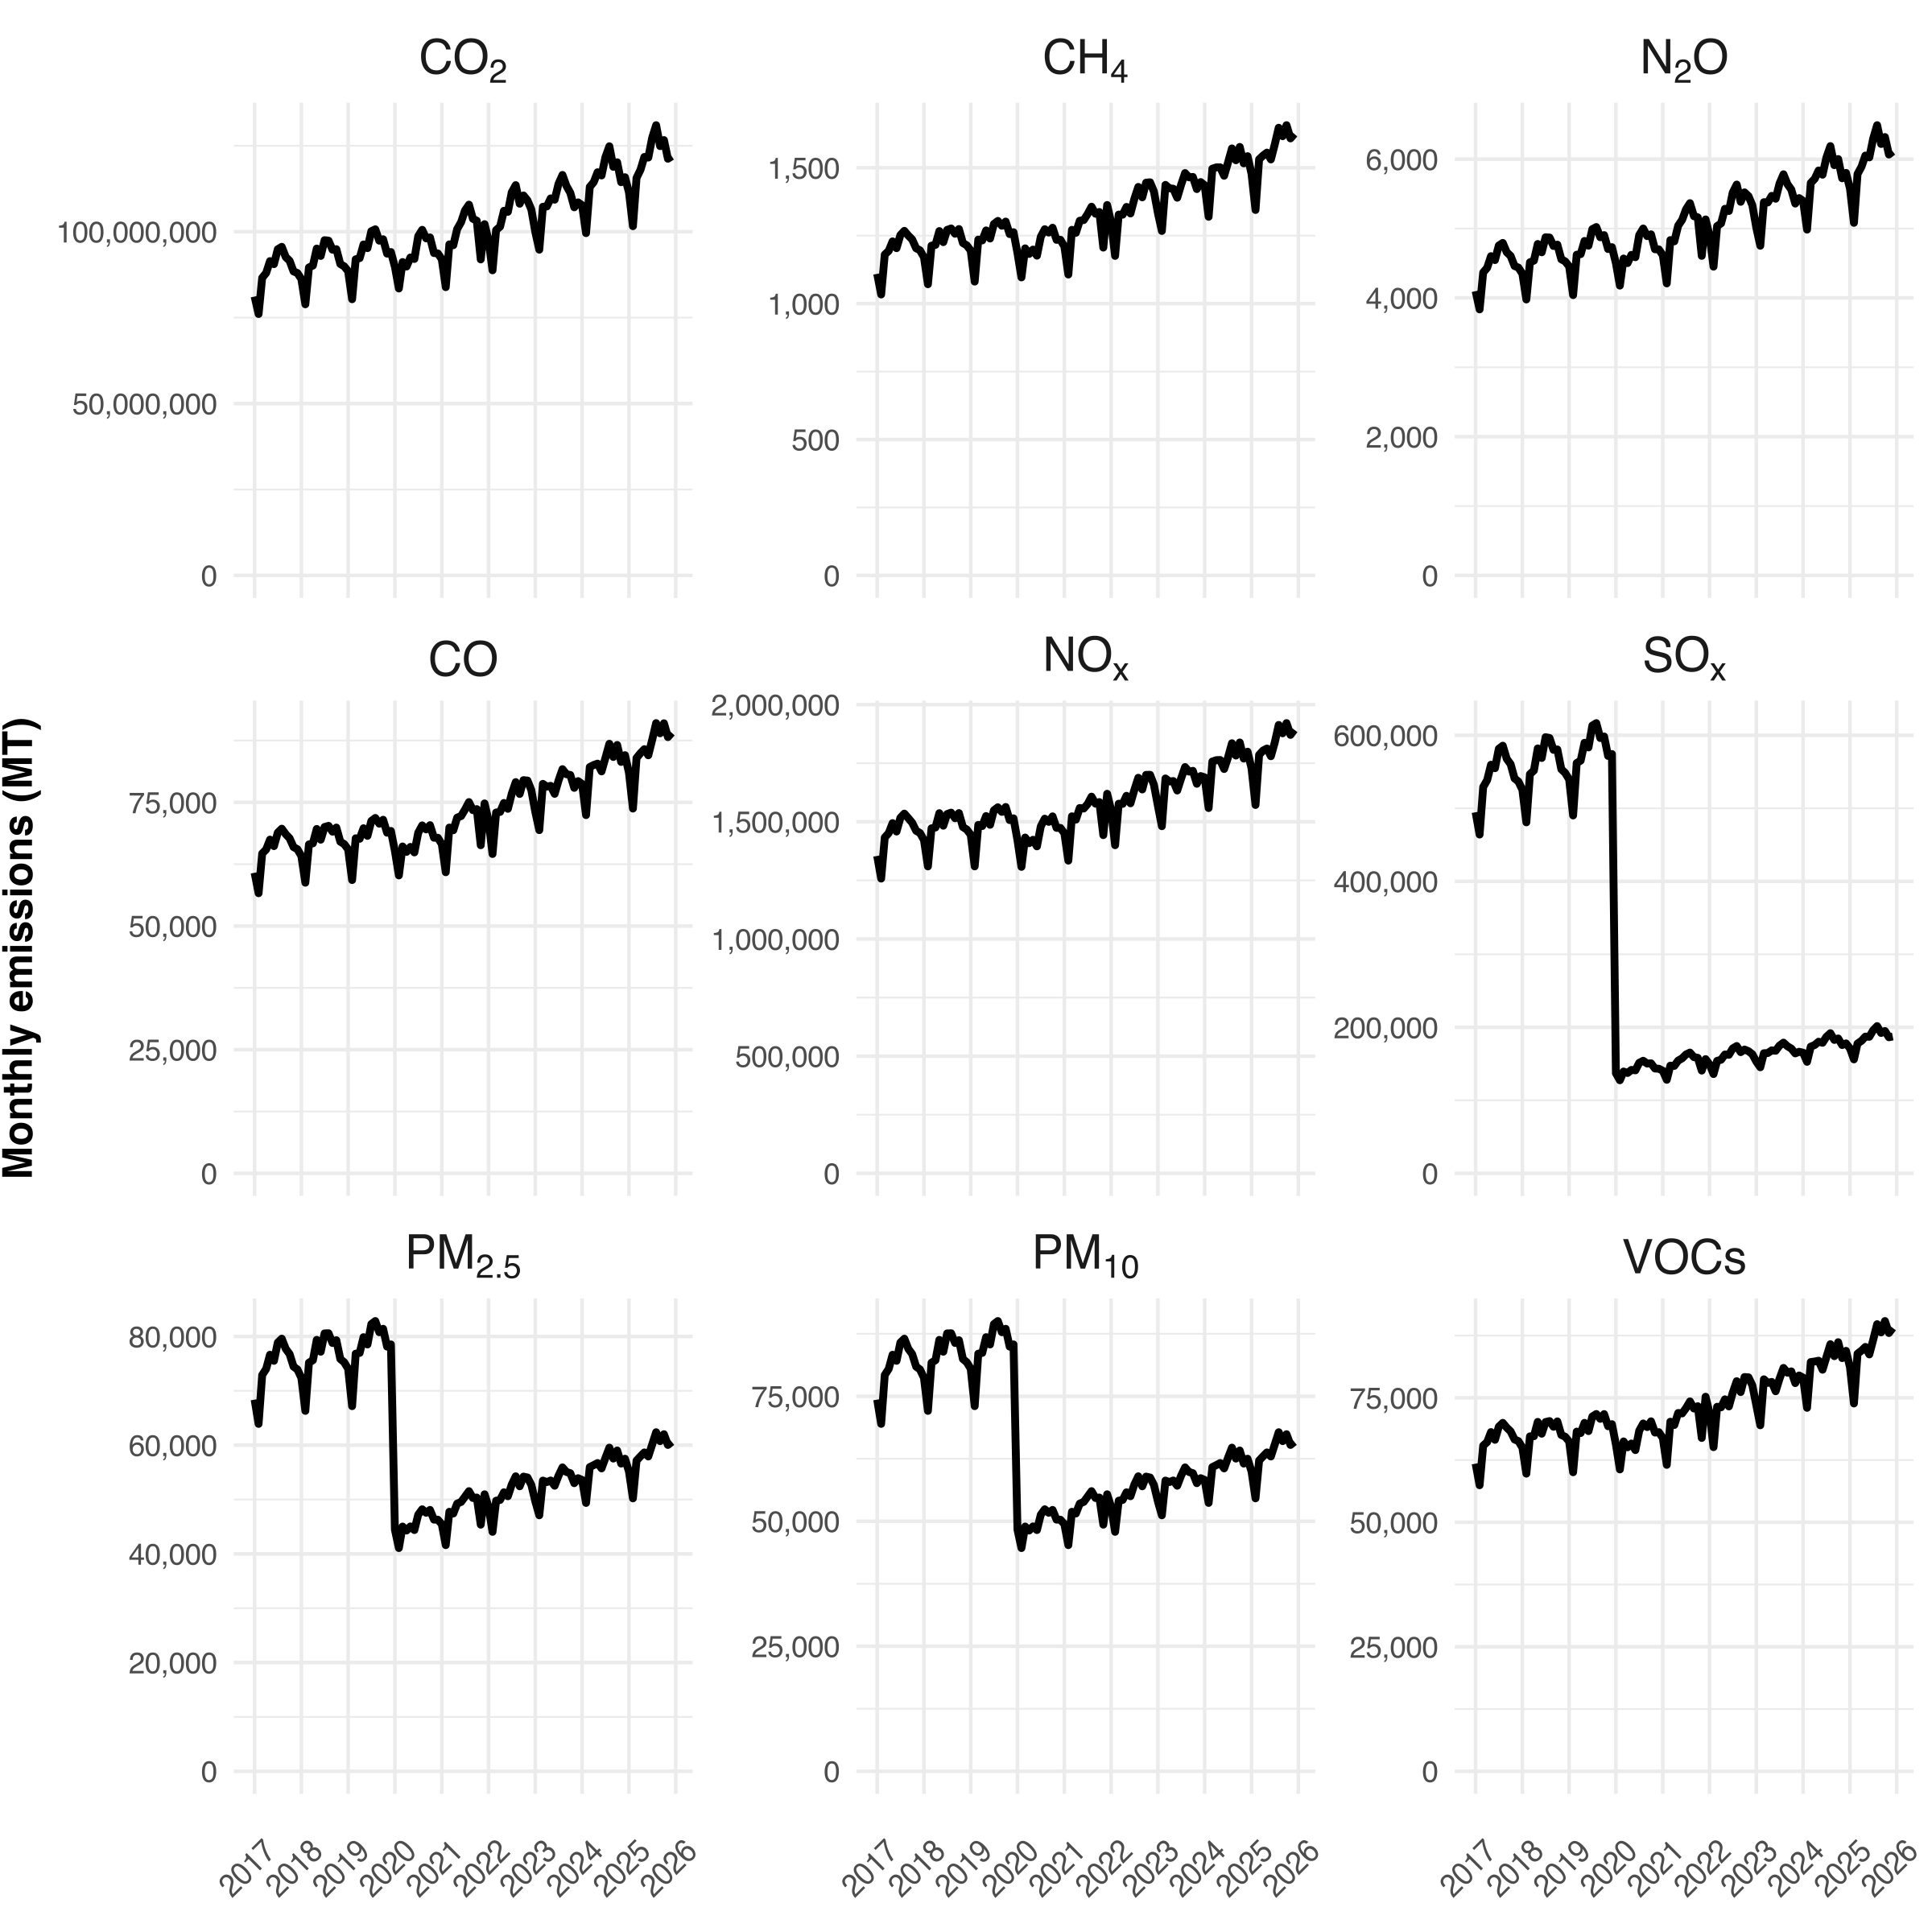
\includegraphics[keepaspectratio]{../figures/fig-pollutant-time-series-1.png}}

}

\caption{\label{fig-pollutant-time-series}Time series of monthly global
emissions for each pollutant, aggregated across AIS-broadcasting vessels
and non-broadcasting vessels.}

\end{figure}%

\subsubsection{Spatial emissions by footprint
group}\label{spatial-emissions-by-footprint-group}

\begin{figure}[H]

\centering{

\pandocbounded{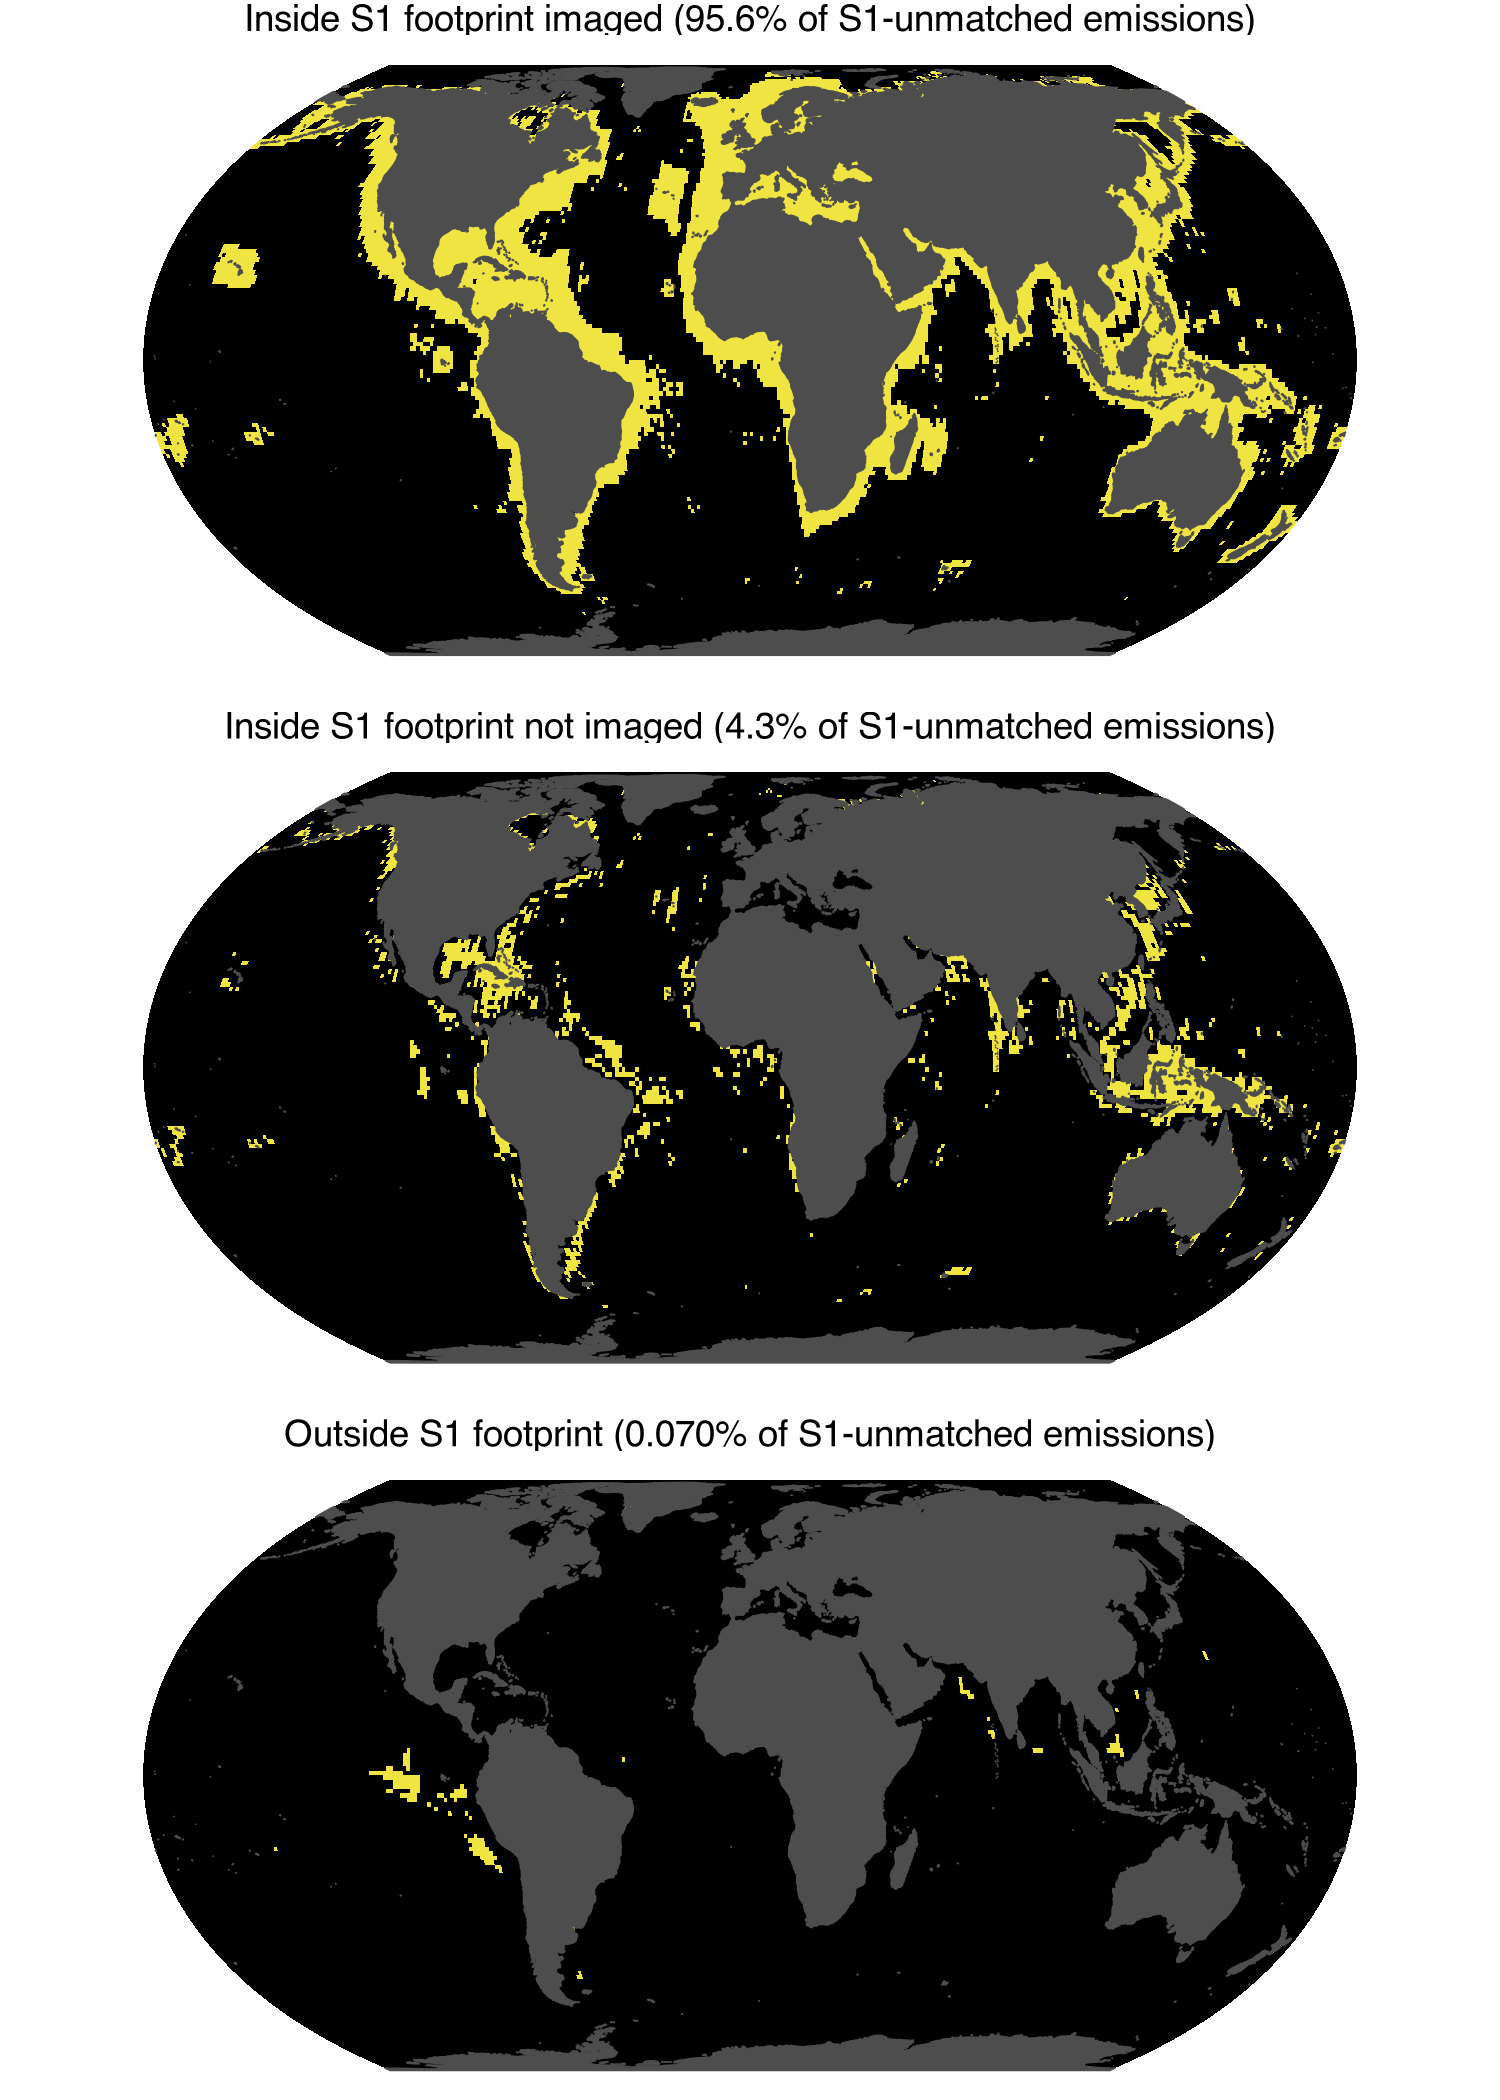
\includegraphics[keepaspectratio]{../figures/fig-spatial-coverage-footprint-1.png}}

}

\caption{\label{fig-spatial-coverage-footprint}Spatial coverage of the
non-broadcasting emissions model. Areas are classified according to
whether they fall inside or outside the S1 footprint and whether they
have been imaged by S1 at any point in time. A given pixel may be imaged
in some months but not in others. Pixels outside the footprint have
never been imaged. The percentage of total CO\(_{2}\) emissions from
non-broadcasting vessels attributed to each category is shown.}

\end{figure}%

\subsubsection{Registered data
validation}\label{registered-data-validation}

\begin{figure}[H]

\centering{

\pandocbounded{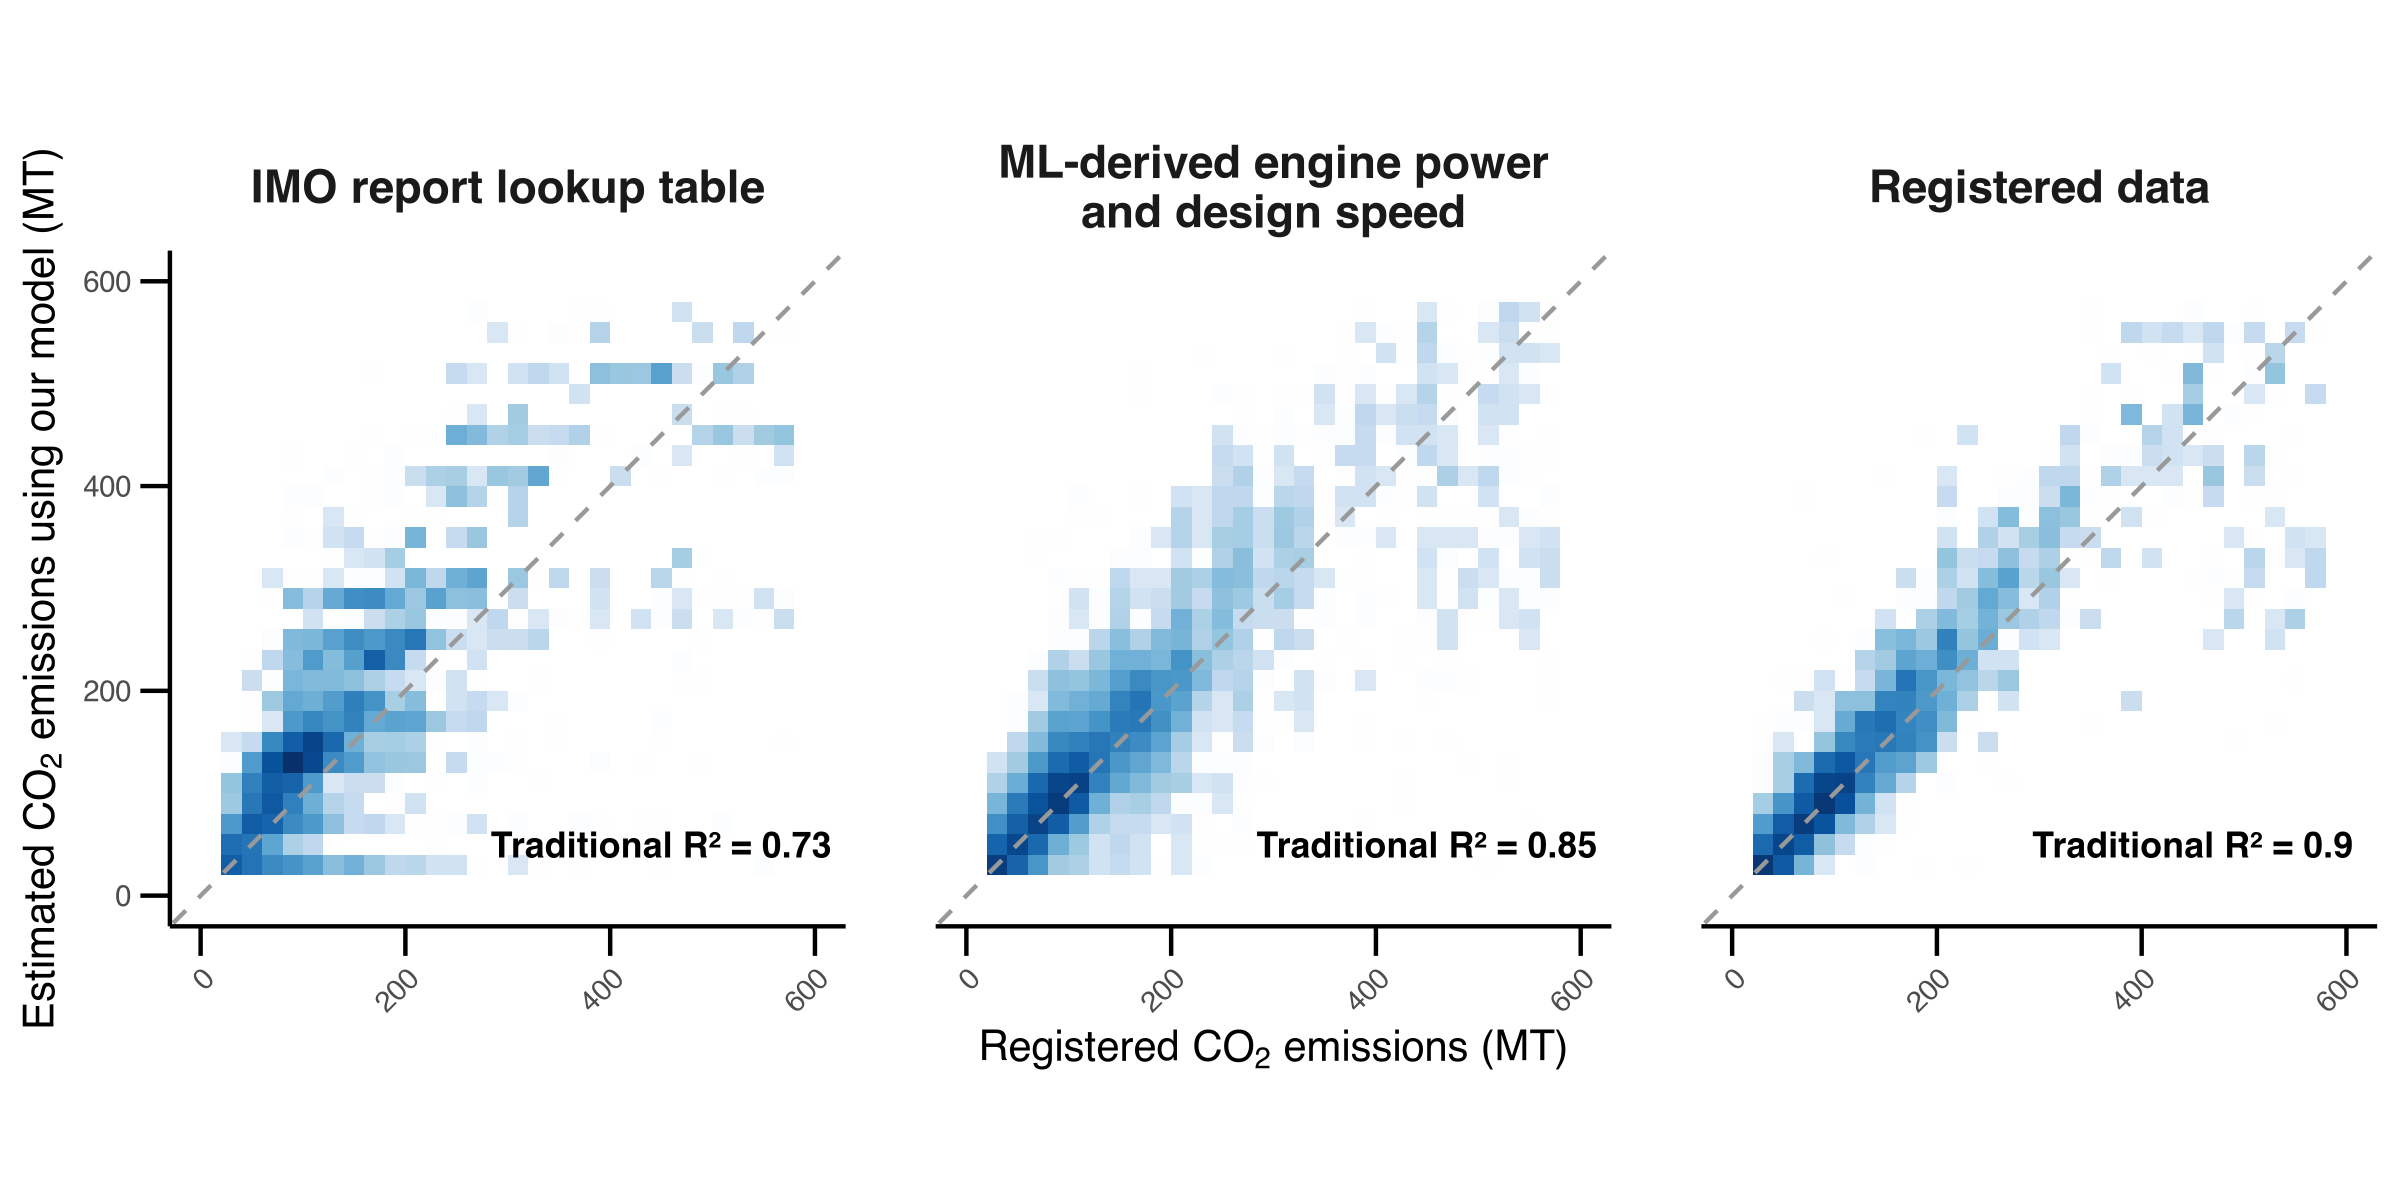
\includegraphics[keepaspectratio]{../figures/fig-registered-data-performance-1.png}}

}

\caption{\label{fig-registered-data-performance}Comparison of registered
and simulated CO\(_{2}\) emissions from main engine fuel consumption
over 24 hours. Estimates are shown using main engine power and design
speed from IMO (left), our machine learning random forest models
(center), and the same registered dataset (right). The solid red line
shows a linear regression fit, while the dashed line represents the 1:1
line. Performance values for traditional R\(^{2}\) are shown for each
set of vessel characteristics. Blue shading indicates point density. All
data are rule-of-three compliant, meaning each cell (20×20 mt) displayed
contains at least three vessels.}

\end{figure}%

\subsubsection{MRV validation}\label{mrv-validation}

\begin{figure}[H]

\centering{

\pandocbounded{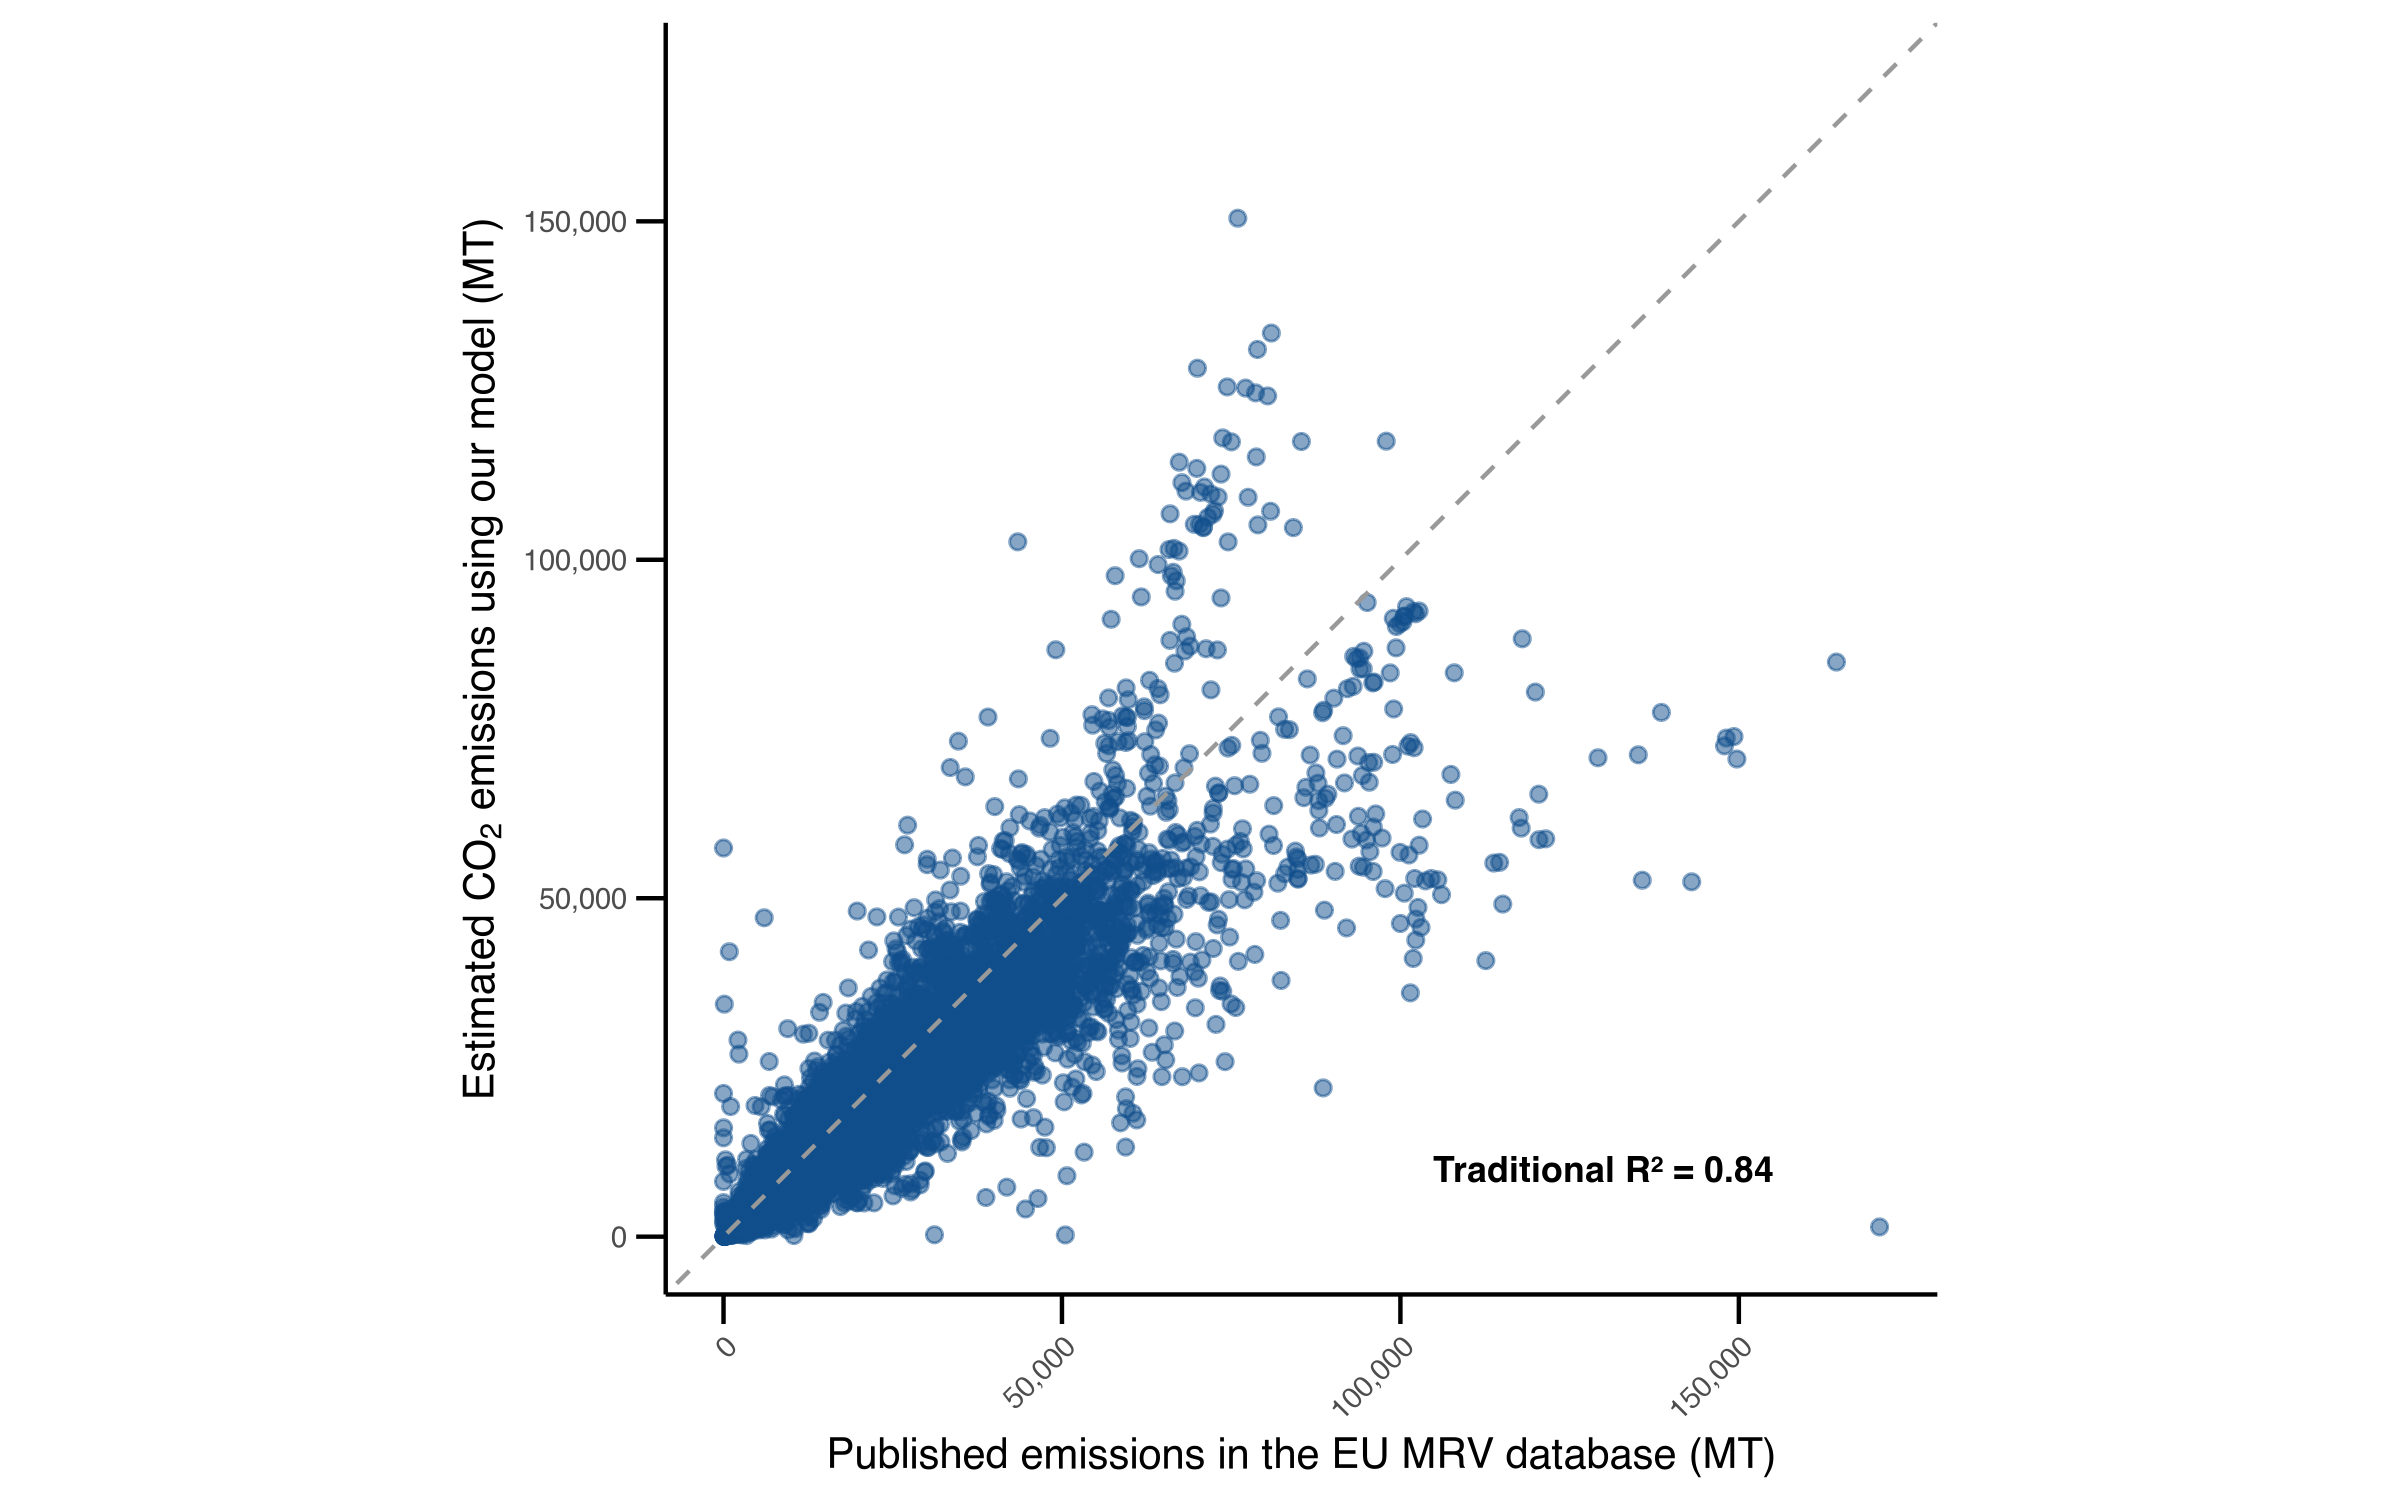
\includegraphics[keepaspectratio]{../figures/fig-mrv-performance-1.png}}

}

\caption{\label{fig-mrv-performance}Comparison of published MRV
emissions and simulated CO\(_{2}\) emissions. The sample includes 2,276
observations from yearly aggregated vessel trips where hours at sea
differ by no more than 15\% between our data and the MRV dataset. The
solid red line shows the linear regression fit, and the dashed line
represents the 1:1 line.\}.}

\end{figure}%

\section{Supplementary tables}\label{supplementary-tables}

\subsection{Dark fleet model performance
metrics}\label{dark-fleet-model-performance-metrics}

\begin{table}[!h]
\centering
\caption{\label{tab:all_performance_metrics_table}Summary of dark fleet model performance metrics for the: 1) emissions regression model; 2) detections classification mode; and 3) detections regression model. Performance estimates for each metric are shown for both the inside S1 footprint and outside S1 footprint tests. All metrics are calculated at the unit of observation except for 'Percent error of total summed predictions', which is the percentage error in the total sum of all predictions relative to the total sum of all truth values.}
\centering
\fontsize{8}{10}\selectfont
\begin{tabular}[t]{l|l|l|r|r}
\hline
Model & Pollutant & Metric & Inside footprint & Outside footprint\\
\hline
Emissions; regression & CO2 & Percent error of total summed predictions & -8.29 & -26.01\\
\hline
Emissions; regression & CO2 & Traditional R² (backtransformed) & 0.94 & 0.69\\
\hline
Emissions; regression & CH4 & Percent error of total summed predictions & -7.78 & -20.62\\
\hline
Emissions; regression & CH4 & Traditional R² (backtransformed) & 0.95 & 0.70\\
\hline
Emissions; regression & N2O & Percent error of total summed predictions & -7.91 & -24.18\\
\hline
Emissions; regression & N2O & Traditional R² (backtransformed) & 0.95 & 0.70\\
\hline
Emissions; regression & CO & Percent error of total summed predictions & -7.93 & -24.01\\
\hline
Emissions; regression & CO & Traditional R² (backtransformed) & 0.95 & 0.69\\
\hline
Emissions; regression & NOX & Percent error of total summed predictions & -7.86 & -27.12\\
\hline
Emissions; regression & NOX & Traditional R² (backtransformed) & 0.95 & 0.67\\
\hline
Emissions; regression & SOX & Percent error of total summed predictions & -8.50 & -28.43\\
\hline
Emissions; regression & SOX & Traditional R² (backtransformed) & 0.94 & 0.68\\
\hline
Emissions; regression & PM2.5 & Percent error of total summed predictions & -7.96 & -25.73\\
\hline
Emissions; regression & PM2.5 & Traditional R² (backtransformed) & 0.95 & 0.69\\
\hline
Emissions; regression & PM10 & Percent error of total summed predictions & -7.90 & -25.62\\
\hline
Emissions; regression & PM10 & Traditional R² (backtransformed) & 0.95 & 0.70\\
\hline
Emissions; regression & VOCs & Percent error of total summed predictions & -8.07 & -18.77\\
\hline
Emissions; regression & VOCs & Traditional R² (backtransformed) & 0.95 & 0.71\\
\hline
Detections; classification & - & Accuracy & 0.85 & 0.87\\
\hline
Detections; classification & - & F1 score & 0.65 & 0.31\\
\hline
Detections; classification & - & Precision-recall AUC & 0.70 & 0.25\\
\hline
Detections; classification & - & Precision & 0.60 & 0.23\\
\hline
Detections; classification & - & recall & 0.70 & 0.49\\
\hline
Detections; classification & - & ROC AUC & 0.89 & 0.79\\
\hline
Detections; classification & - & Sensitivity & 0.70 & 0.49\\
\hline
Detections; classification & - & Specificity & 0.89 & 0.89\\
\hline
Detections; regression & - & Traditional R² & 0.78 & 0.10\\
\hline
\end{tabular}
\end{table}

\subsection{Summary of 2017 and 2024 emissions, by pollutant and data
source}\label{summary-of-2017-and-2024-emissions-by-pollutant-and-data-source}

\subsection{Underestimation of 2024 emissions using only AIS data, and
overestimation of 2017 to 2024 emissions trend using only AIS data, by
pollutant.}\label{underestimation-of-2024-emissions-using-only-ais-data-and-overestimation-of-2017-to-2024-emissions-trend-using-only-ais-data-by-pollutant.}

\subsubsection{Feature importance}\label{feature-importance}

\begin{figure}[H]

\centering{

\pandocbounded{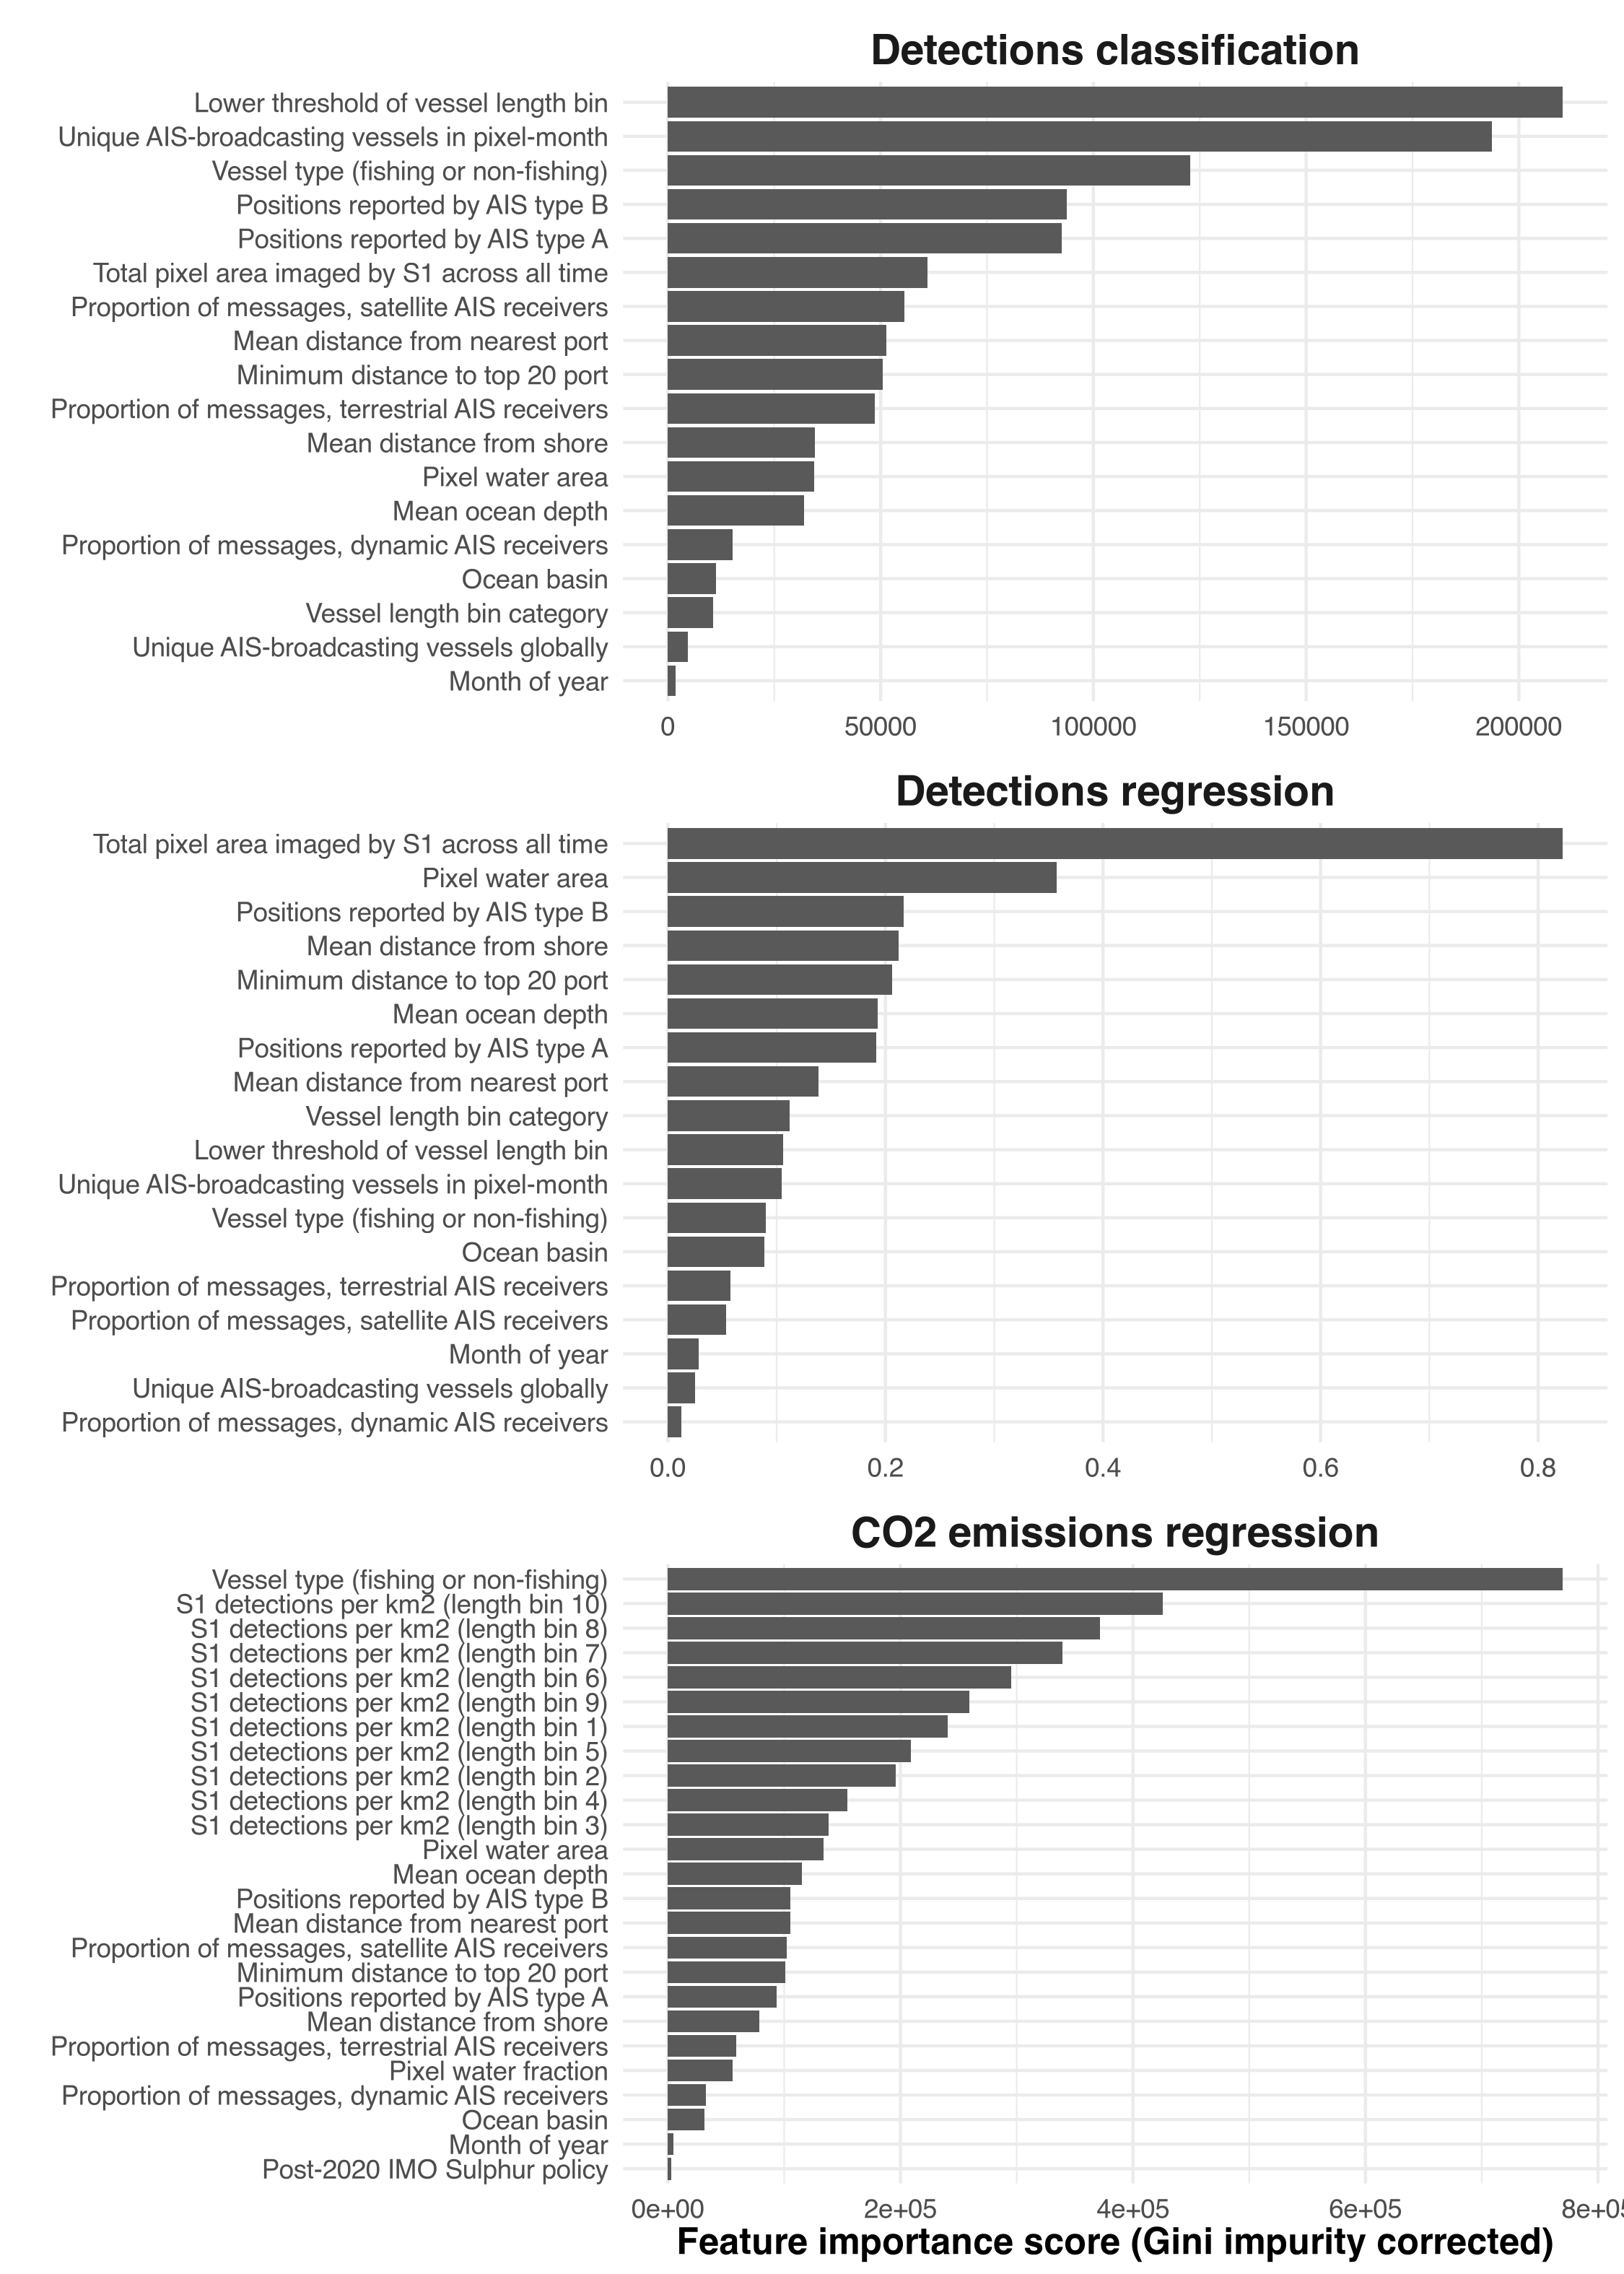
\includegraphics[keepaspectratio]{../figures/fig-feature-importance-1.png}}

}

\caption{\label{fig-feature-importance}Feature importance plots for the
three final model fit random forests}

\end{figure}%

\subsubsection{Classification model
performance}\label{classification-model-performance}

\begin{figure}[H]

\centering{

\pandocbounded{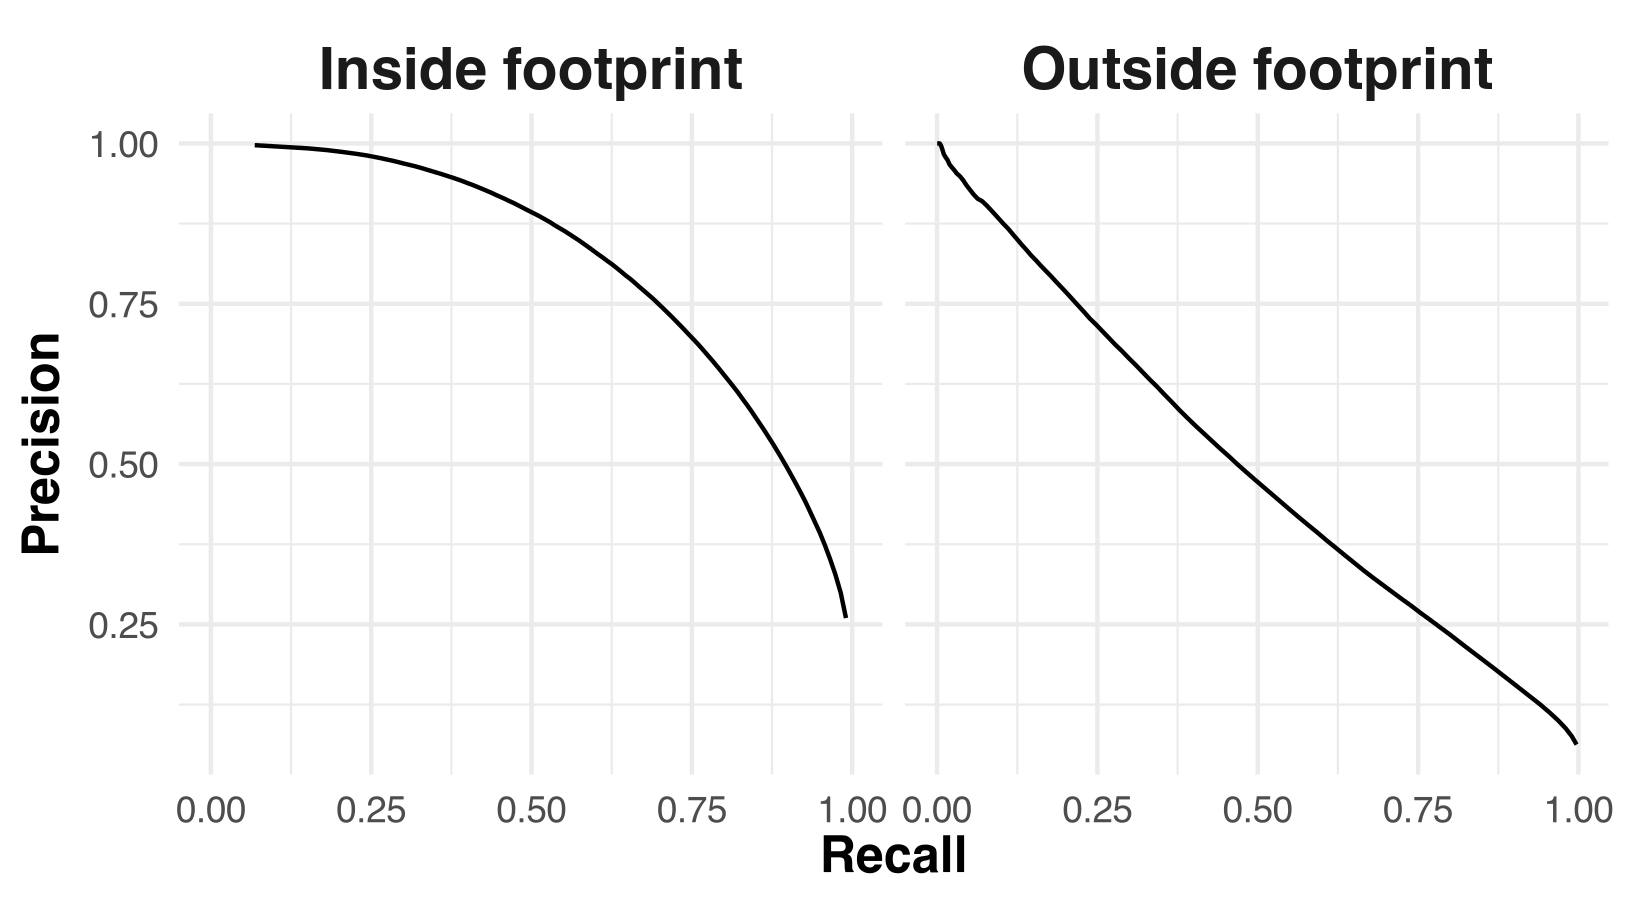
\includegraphics[keepaspectratio]{../figures/fig-pr-curves-1.png}}

}

\caption{\label{fig-pr-curves}Precision recall curves for the detection
classification model, shown for the inside S1 footprint and outside S1
footprint performance tests}

\end{figure}%

\begin{figure}[H]

\centering{

\pandocbounded{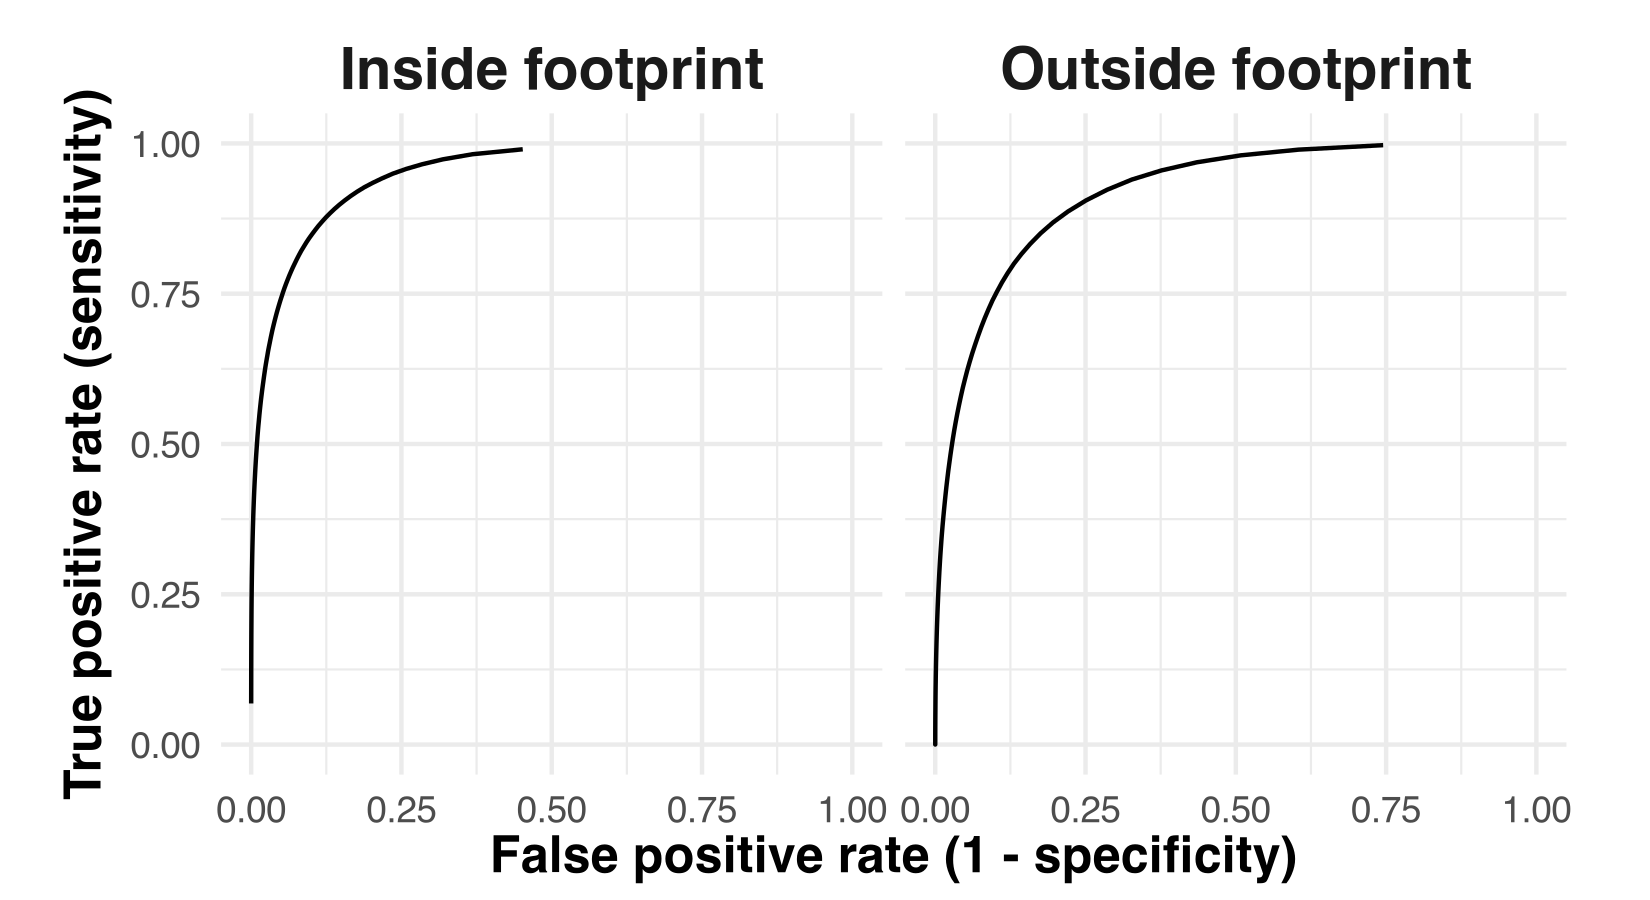
\includegraphics[keepaspectratio]{../figures/fig-roc-curves-1.png}}

}

\caption{\label{fig-roc-curves}ROC curves for the detection
classification model, shown for the inside S1 footprint and outside S1
footprint performance tests}

\end{figure}%

\begin{figure}[H]

\centering{

\pandocbounded{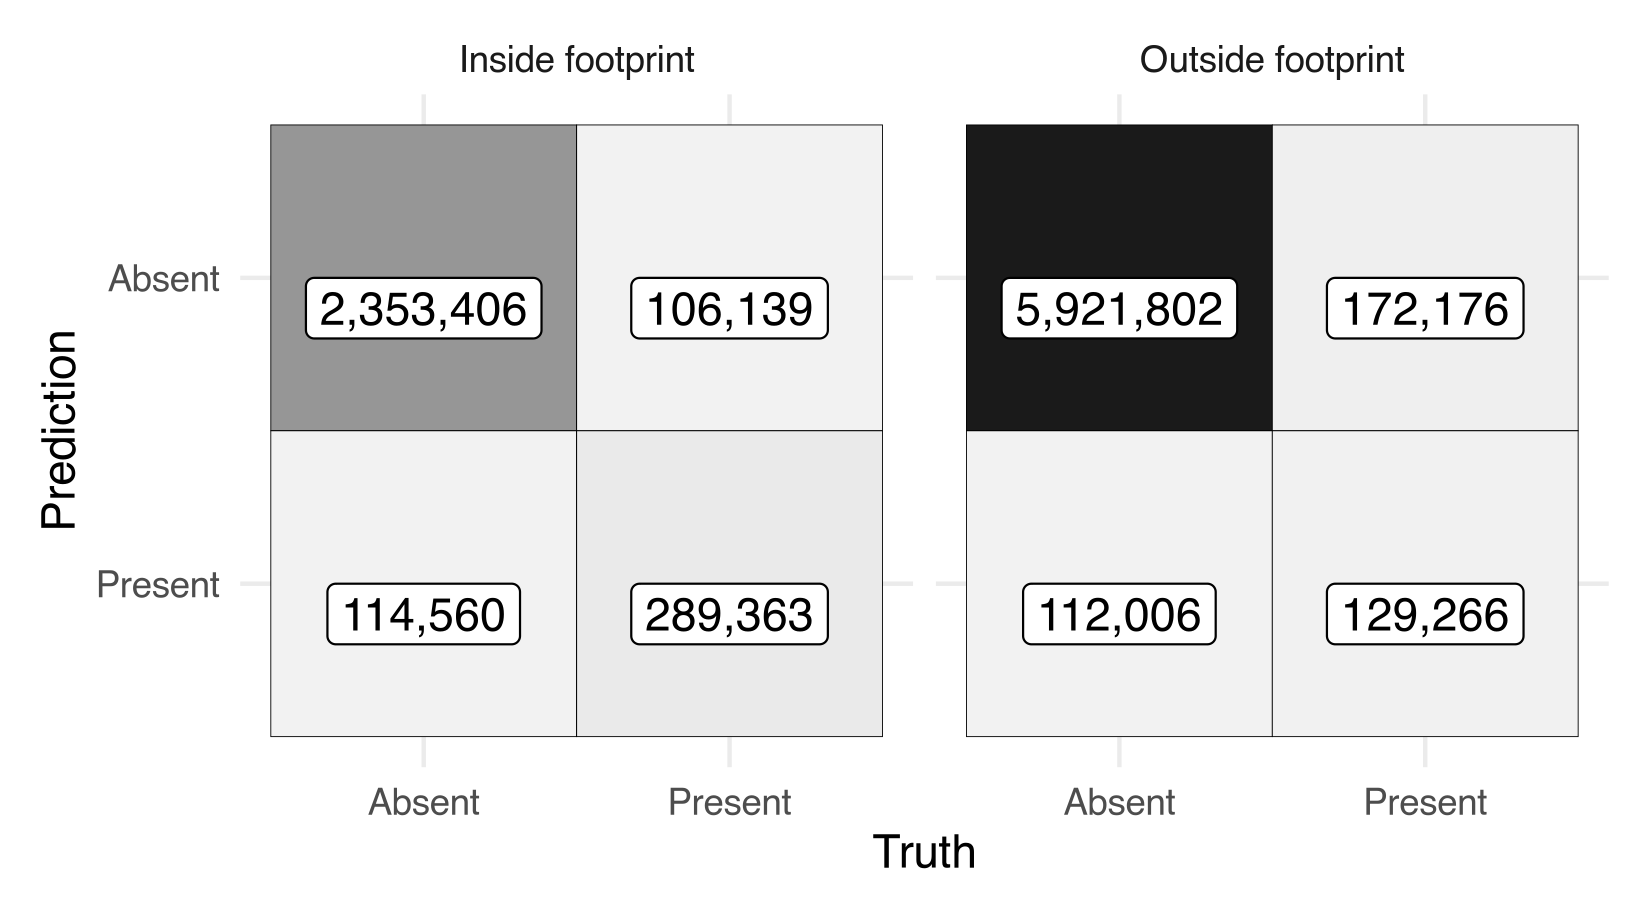
\includegraphics[keepaspectratio]{../figures/fig-conf-mat-1.png}}

}

\caption{\label{fig-conf-mat}Confusion matricies for the detection
classification model, shown for the inside S1 footprint and outside S1
footprint performance tests}

\end{figure}%

\subsubsection{Dynamic AIS - annual emissions and vessels by AIS
receiver
type}\label{dynamic-ais---annual-emissions-and-vessels-by-ais-receiver-type}

\begin{figure}[H]

\centering{

\pandocbounded{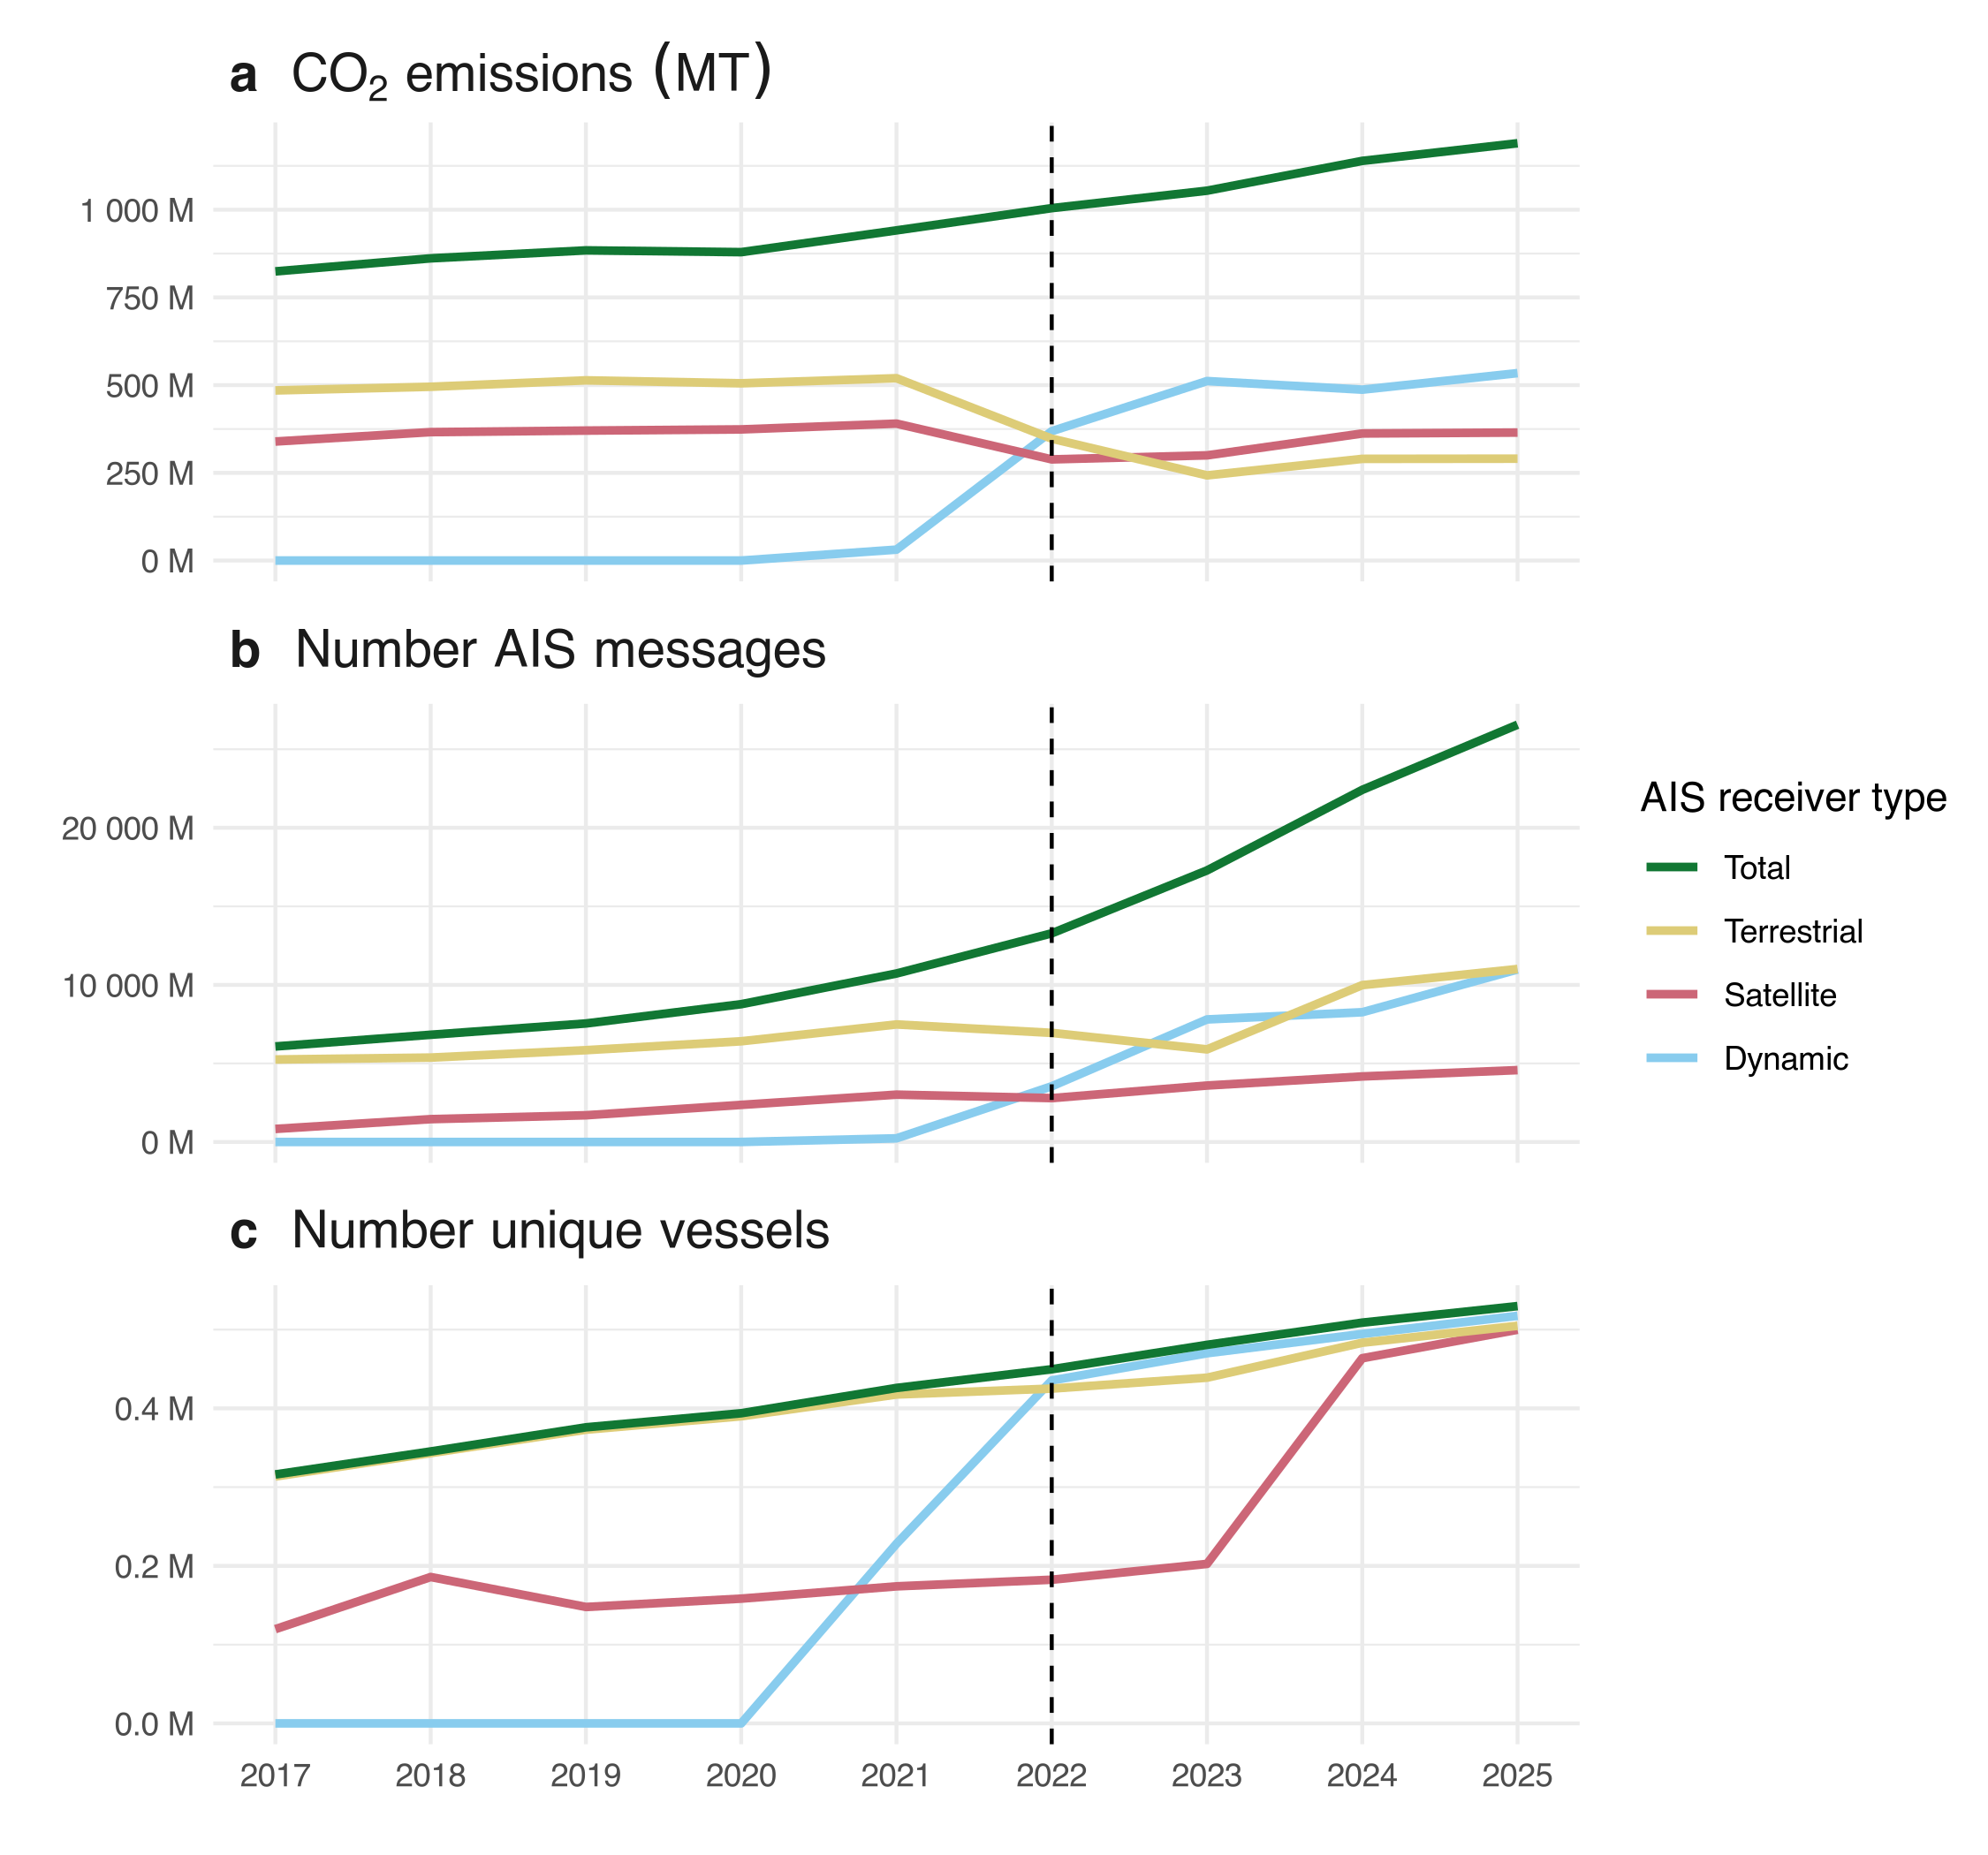
\includegraphics[keepaspectratio]{../figures/fig-annual-emissions-by-ais-receiver-type-1.png}}

}

\caption{\label{fig-annual-emissions-by-ais-receiver-type}Annual total
CO2 emissions (metric tonnes) by the AIS-broadcasting fleet,
disaggregated by AIS receiver type (satellite, terrestrial, and dynamic)
and total aggregated across receiver types. A dashed vertical line is
shown for 2022, the first year in which dynamic AIS was widely adopted.}

\end{figure}%

\subsubsection{Dynamic AIS - annual emissions by AIS receiver type for
top
flags}\label{dynamic-ais---annual-emissions-by-ais-receiver-type-for-top-flags}

\begin{figure}[H]

\centering{

\pandocbounded{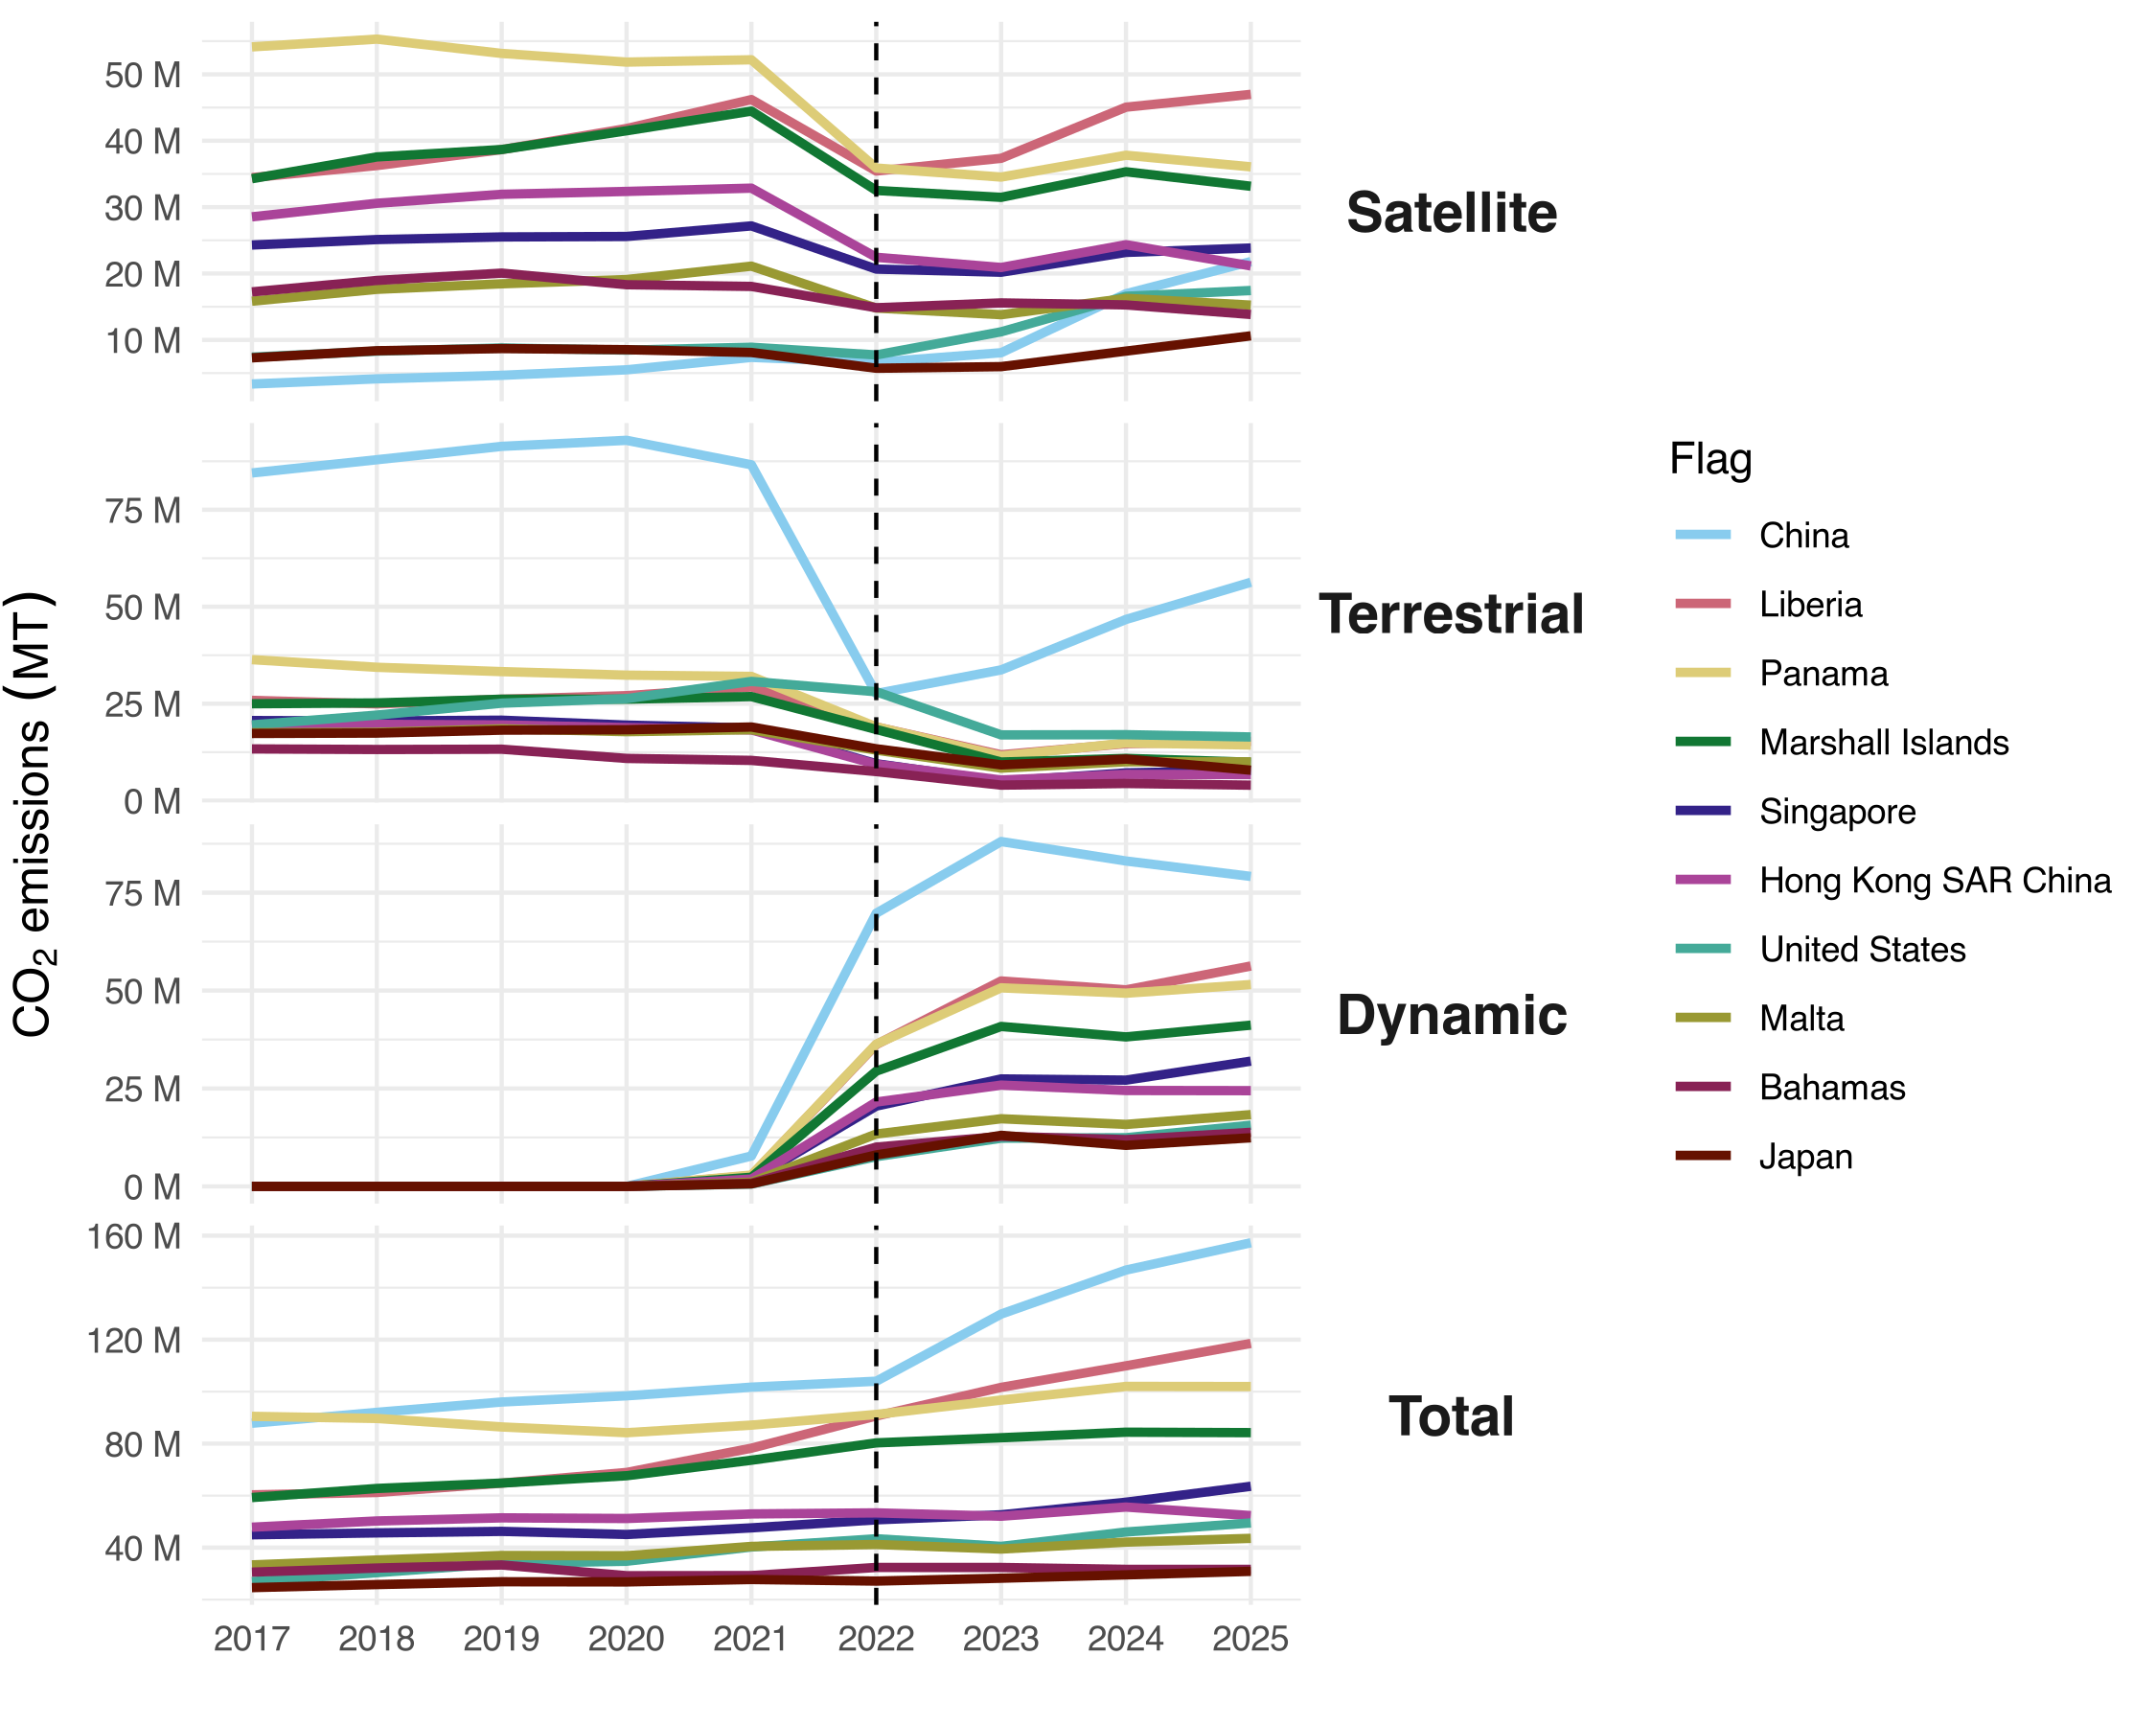
\includegraphics[keepaspectratio]{../figures/fig-annual-emissions-by-ais-receiver-type-top-flags-1.png}}

}

\caption{\label{fig-annual-emissions-by-ais-receiver-type-top-flags}Annual
total CO2 emissions (metric tonnes) by the AIS-broadcasting fleet,
disaggregated by AIS receiver type (satellite, terrestrial, and dynamic)
and total aggregated across receiver types, for the top 10 flags with
the most emissions in 2024. A dashed vertical line is shown for 2022,
the first year in which dynamic AIS was widely adopted.}

\end{figure}%

\subsubsection{Dynamic AIS - map showing spatial change in emissions by
AIS receiver
type}\label{dynamic-ais---map-showing-spatial-change-in-emissions-by-ais-receiver-type}

\begin{figure}[H]

\centering{

\pandocbounded{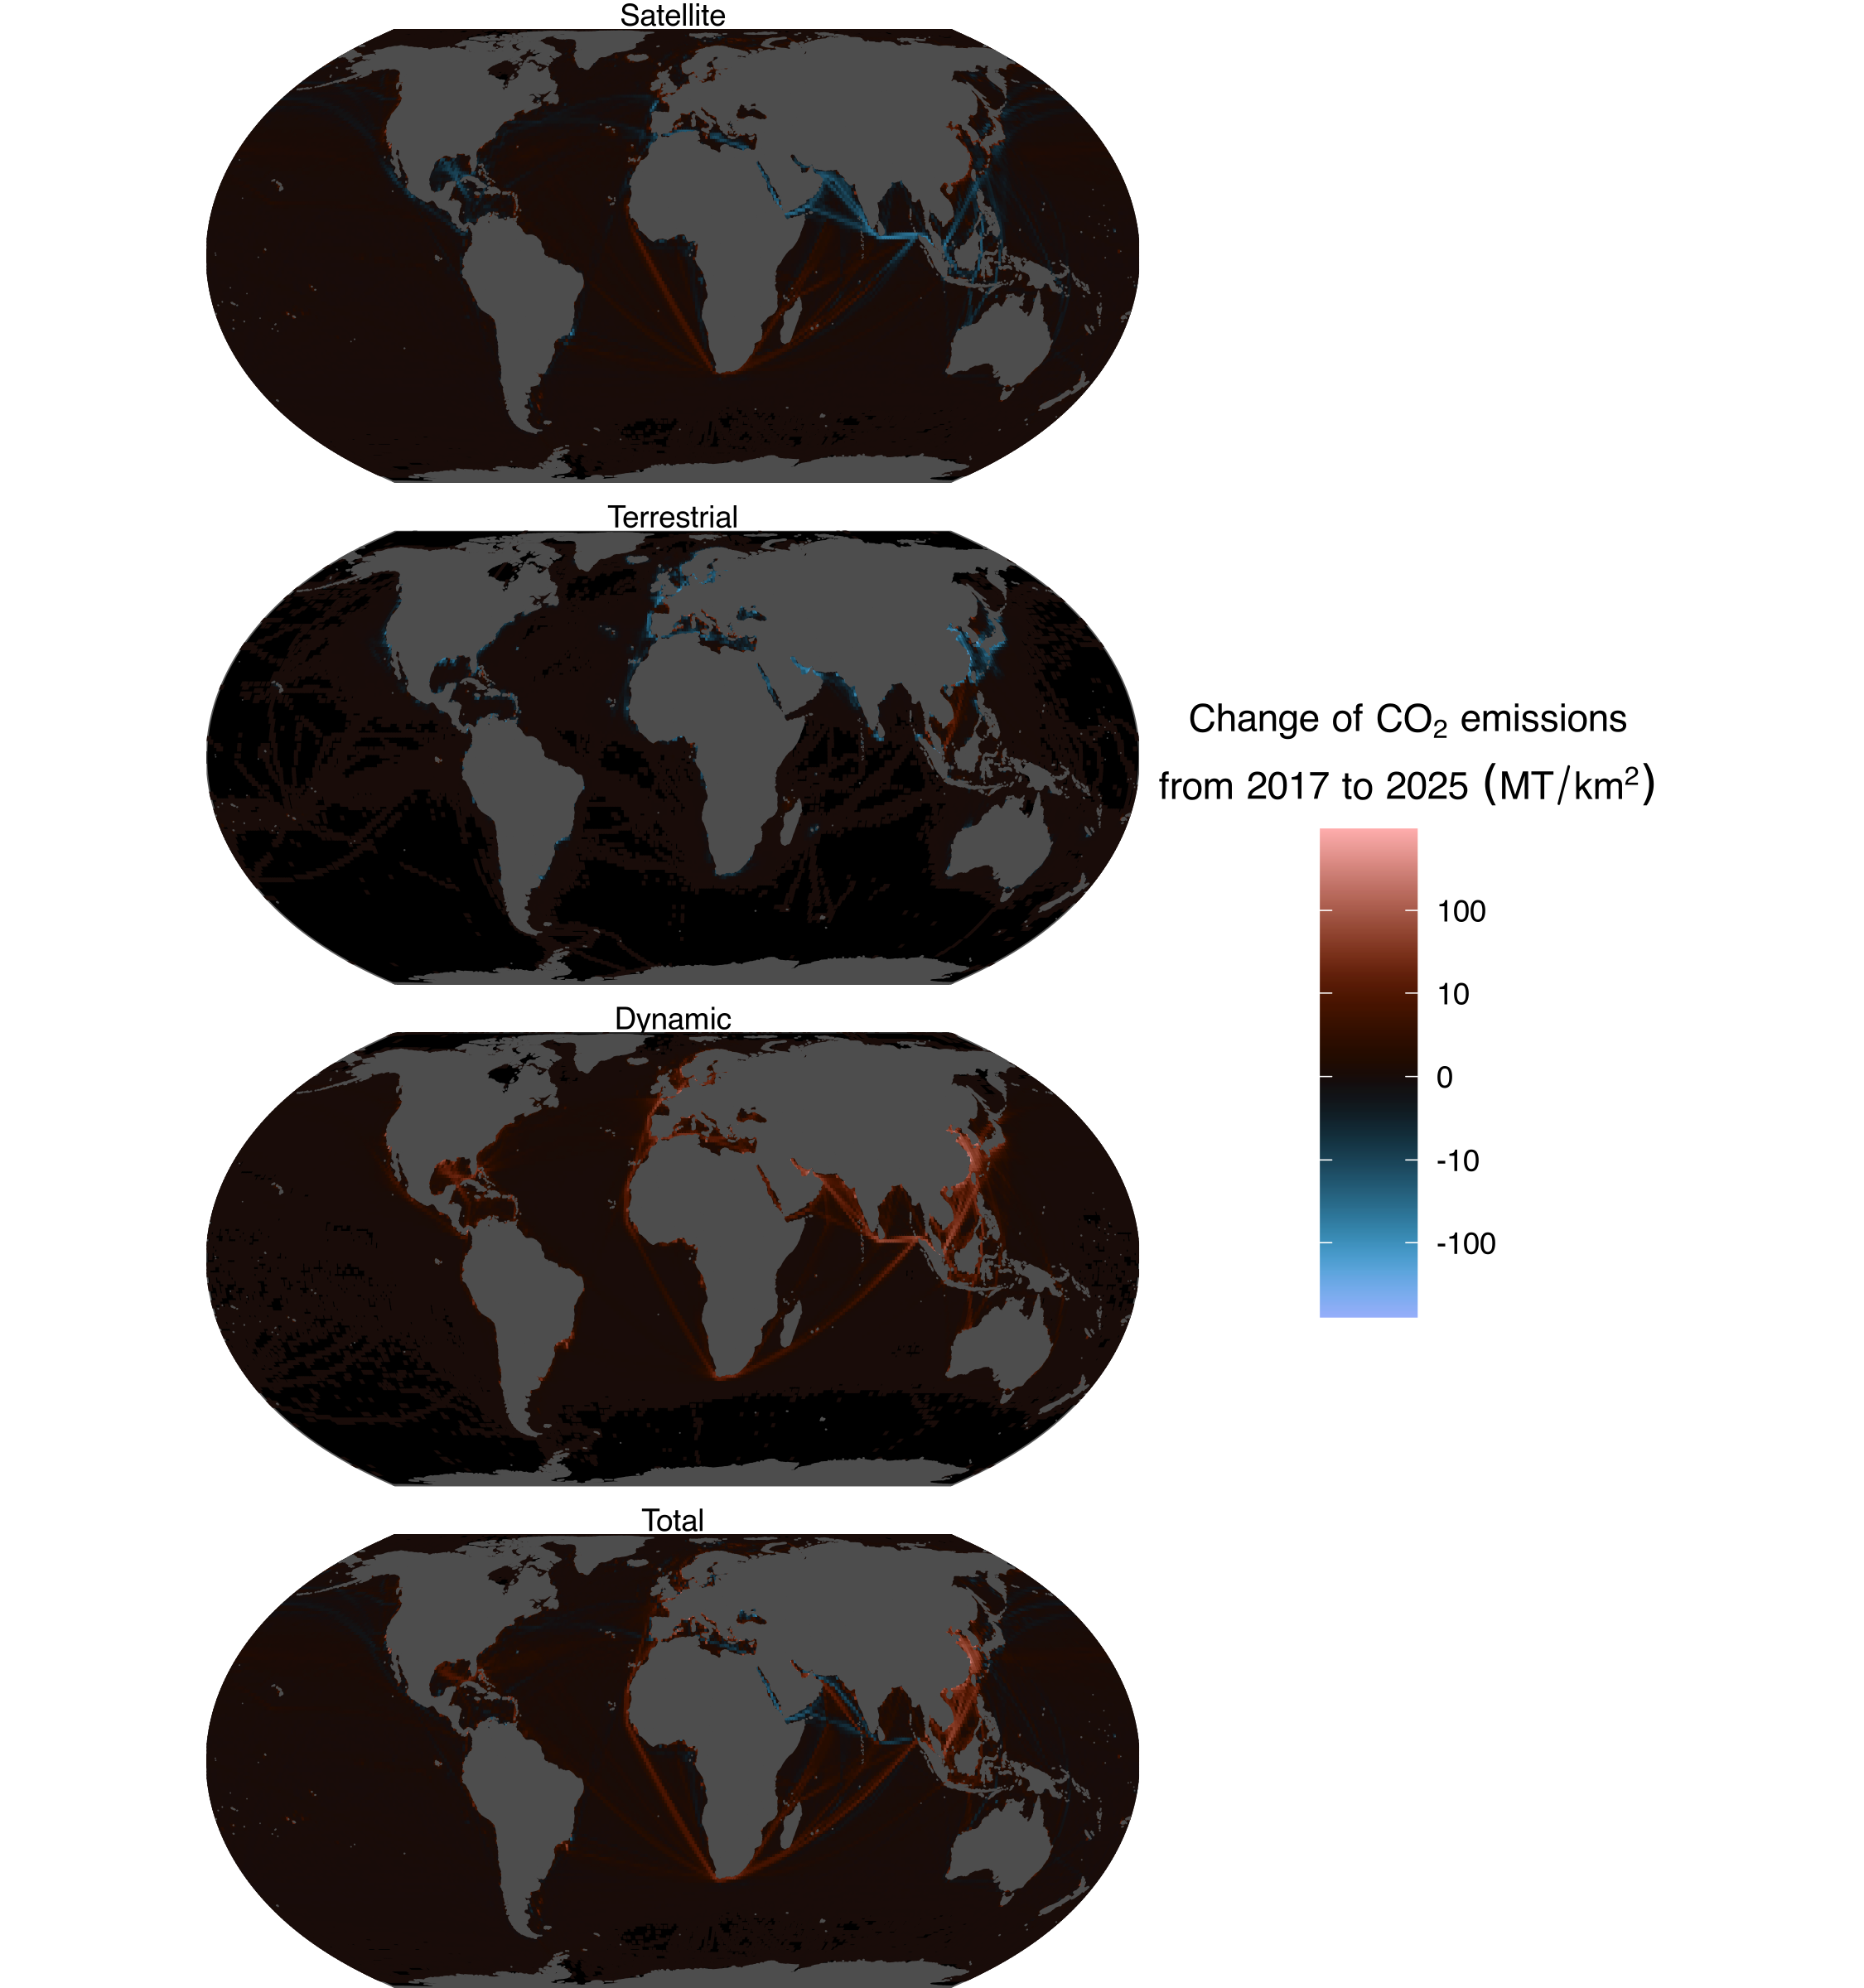
\includegraphics[keepaspectratio]{../figures/fig-co2-emissions-change-map-by-receiver-type-1.png}}

}

\caption{\label{fig-co2-emissions-change-map-by-receiver-type}Spatial
change in CO2 emissions by the AIS-broadcasting fleet between 2017 and
2024 (metric tonnes) by receiver type (satellite, terrestrial, and
dynamic) and total across receiver types, at a 1x1 degree spatial
resolution.}

\end{figure}%

\#\#~MRV performance validation table

\section{Non-broadcasting model data
sources}\label{non-broadcasting-model-data-sources}

\begin{figure}[H]

\centering{

\pandocbounded{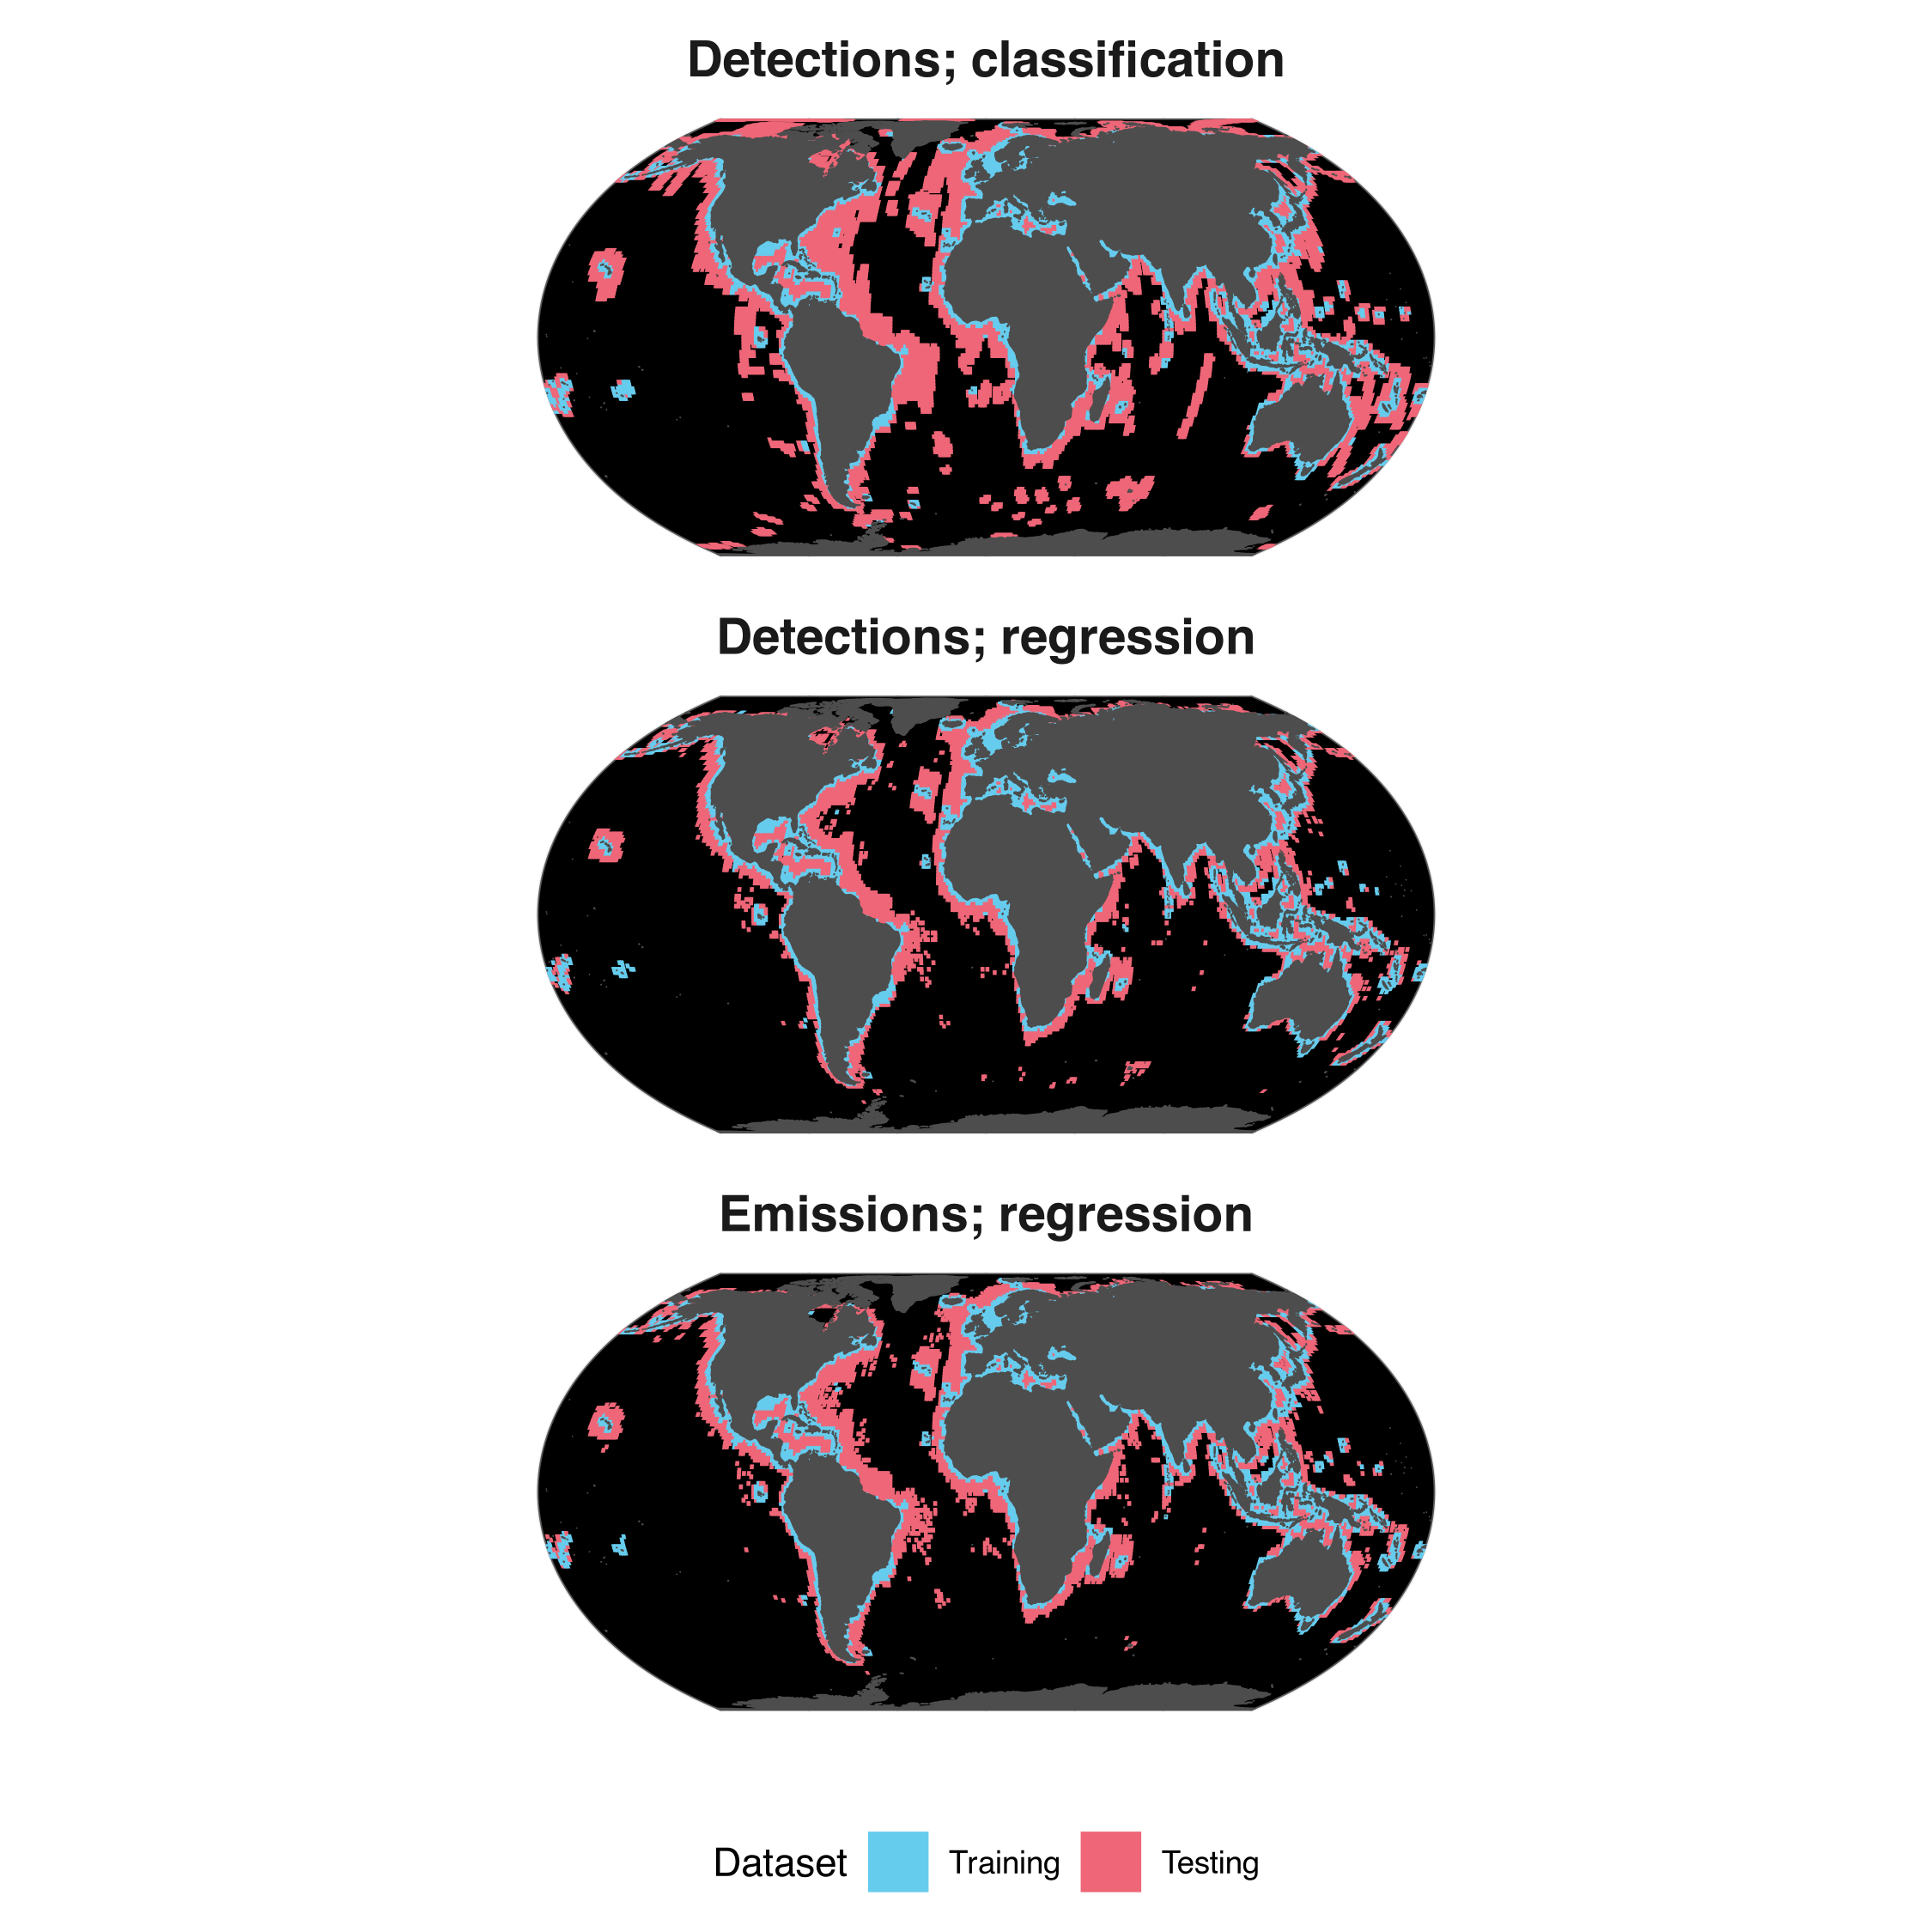
\includegraphics[keepaspectratio]{../figures/fig-offshore-outside-footprint-training-testing-map-1.png}}

}

\caption{\label{fig-offshore-outside-footprint-training-testing-map}Maps
of pixels that were used in the training and testing datasets for the
outside S1 performance tests for each model. Pixels \textless=100km from
the shore were used for training; pixels \textgreater100km from shore
were used for testing. The exact training/testing split for each of the
3 models is shown.}

\end{figure}%




\end{document}
